\documentclass[journal]{IEEEtran}
%\IEEEoverridecommandlockouts
%\documentclass[onecolumn, 10pt, draftclsnofoot]{IEEEtran}
\usepackage{graphicx}
\usepackage{cite}
\usepackage{picinpar}
\usepackage{amsmath}
\usepackage{url}
\usepackage{multicol}
%\usepackage{flushend}
\usepackage[latin1]{inputenc}
\usepackage{colortbl}
\usepackage{soul}
\soulregister\cite7
\soulregister\eqref7
\soulregister\citep7
\soulregister\citet7
\soulregister\ref7
\soulregister\pageref7
\usepackage{multirow}
\usepackage{pifont}
\usepackage{color}
\usepackage{alltt}
\usepackage{float}
\usepackage[hidelinks]{hyperref}
\usepackage{enumerate}
\usepackage{siunitx}
%\usepackage{breakurl}
\usepackage{amsmath}
\usepackage{epstopdf}
\usepackage{pbox}
\usepackage{afterpage}
\usepackage{verbatim}
\usepackage{amssymb}
\usepackage{multirow}
\usepackage{booktabs}
\usepackage{stfloats}
\usepackage{makecell}
\usepackage{balance}
\usepackage{threeparttable}
%\usepackage{extpfeil}
%\usepackage{caption}
\usepackage{subfigure}
\usepackage{empheq}
\usepackage{lipsum}
\usepackage{cuted}\stripsep -3pt plus 3pt minus 2pt
\usepackage{steinmetz}
\def\hrulefill{\leavevmode\leaders\hrule height 0.8pt\hfill\kern0pt}
\makeatletter
\def\rulefill{\leavevmode\leaders\hrule depth -3pt height 4pt\hfill\kern0pt}
\makeatother
\usepackage{array}


\begin{document}
\title{
Analysis and Implementation of 3D Magnetic Field Shaping via A 2D Planar Transmitting Coil Array
}

\author{
Ning~Kang,~\IEEEmembership{Student Member,~IEEE,}
Yaoxia~Shao,~\IEEEmembership{Student Member,~IEEE,}\\
Ming~Liu,~\IEEEmembership{Senior Member,~IEEE,}
Chengbin~Ma,~\IEEEmembership{Senior Member,~IEEE}
\vspace{-0.3cm}
\thanks{$\copyright$ 2021 IEEE. Personal use of this material is permitted. Permission from IEEE must be obtained for all other uses, including reprinting/republishing this material for advertising or promotional purposes, collecting new collected works for resale or redistribution to servers or lists, or reuse of any copyrighted component of this work in other works.}

\thanks{Manuscript received Apr. 24, 2021; revised Jul. 9, 2021; accepted Jul. 30, 2021. This work was supported by National Natural Science Foundation of China under Grant 52077132. {\it (Corresponding author: Chengbin Ma)}}

\thanks{N.~Kang, Y.~Shao, and C.~Ma are with the University of Michigan-Shanghai Jiao Tong University Joint Institute, Shanghai Jiao Tong University, Shanghai 200240, P. R. China (e-mail: corningkdc@sjtu.edu.cn; yaoxiashao@sjtu.edu.cn; chbma@sjtu.edu.cn).}

\thanks{M.~Liu is with the Key Laboratory of Control of Power Transmission and Conversion of Ministry of Education, and the School of Electronic Information and Electrical Engineering, Shanghai Jiao Tong University, Shanghai 200240, China (e-mail: mingliu@sjtu.edu.cn).}}

%\vspace{-0.5cm}
\maketitle


\begin{abstract}
	Wireless power transfer (WPT) systems operating at several MHz are known to be advantageous for realizing high spatial freedom of power transfer and compact/lightweight designs. The combined use of multiple transmitting (Tx) coils for magnetic field shaping is expected to further increase the spatial freedom.
	This paper studies an extendable planar Tx-coil array architecture. This architecture provides new conveniences for the MHz WPT systems to efficiently charge devices in 3D space.
	Time-domain and phasor-domain modelings are carried out in turn to analyze the magnetic field shaping effect under the current phase shift modulation of the Tx coils.
	An overlap design of the Tx-coil layout is also developed to minimize the cross coupling between the coils, which reduces the interference between Tx coils. Finally, the above concepts are experimentally implemented. The results clearly demonstrate the new advantages of the planar Tx-coil array-based magnetic field shaping, in terms of spatial freedom of the power transfer, efficiency, and output power capability, when charging receivers with six-degrees-of-freedom positions and orientations in 3D space. For instance, a perpendicular receiver in the center of the Tx-coil array can be charged with 82\% dc-dc efficiency and 45~W, which is difficult for a conventional single Tx-coil solution.
\end{abstract}

\begin{IEEEkeywords}
Cross coupling minimization, magnetic field shaping, planar transmitting-coil array, 3D space, wireless power transfer.
\end{IEEEkeywords}

\definecolor{limegreen}{rgb}{0.2, 0.8, 0.2}
\definecolor{forestgreen}{rgb}{0.13, 0.55, 0.13}
\definecolor{greenhtml}{rgb}{0.0, 0.5, 0.0}

\section{Introduction}

Wireless power transfer (WPT) has attracted great interest in recent years due to the significantly enhanced convenience in charging various electronic devices and even electric vehicles. Most commercial WPT systems operate in the kilohertz (kHz) band~\cite{Qi2016wireless,SAE2016wireless}. Many efforts have been made to improve the performance of the kHz systems through innovations in circuit topology, coil design and control~\cite{kan2016new,mi2016modern,hua2018modeling}. At the same time, a higher operating frequency, such as several megahertz (MHz), is promising to achieve a higher degree of spatial freedom in power transfer and a compact and lightweight design~\cite{Soljacic_science,liu2020high,aldhaher2018load}. As same as the kHz WPT, the ever-increasing requirement for the spatial freedom also poses challenges for the MHz WPT, especially when charging devices with different positions and orientations in three-dimensional (3D) space. Many investigations have been conducted such as through adopting repeaters, impedance matching networks, new coil structures and switching devices~\cite{kim2011efficiency,lim2013adaptive,zhao2017gan,zhang2018wireless}. In conventional WPT systems, the magnetic field (i.e., B-field) distribution is usually regraded as uncontrollable, which depends mostly on the design of transmitting (Tx) coil. For instance, different single 3D Tx coils have been proposed to generate an omnidirectional magnetic field~\cite{kim2015free,ha2017analytical}. In addition, direct-quadrature (DQ) Tx coils with ferrite cores were applied to achieve wide-range omnidirectional inductive power transfer~\cite{choi2015six,lee2018modularized}. Specially designed 3D receiving (Rx) coils were also developed to reduce the spatial output power variation~\cite{park2013two,zhang2019angular}. 
\IEEEpubidadjcol

Through multiple Tx coils and appropriate control, it is possible to actively shape the B-field distribution in 3D space. This provides an important new degree of freedom to further enhance the performance (e.g., transfer distance, efficiency and power transfer capability) of today's MHz WPT systems. Majority of existing work on the magnetic field shaping operated in the kHz band, and many of those investigations adopted 3D structures of orthogonal Tx coils, which can straightforwardly avoid cross coupling between Tx coils~\cite{ng2014two,zhang2019angular,lim2014novel,tang2019simultaneous}. For instance, nonidentical current control for two-dimensional (2D) and 3D omnidirectional WPT has been proposed and implemented~\cite{ng2014two}. A spherical shape transmitter structure was adopted consisting of two or three separate orthogonal Tx coils and worked at 530~kHz. With the similar transmitter structure, a quadrature-shaped receiving (Rx) coil was further developed to achieve an angular-misalignment insensitive 100~kHz WPT system~\cite{zhang2019angular}. Using two orthogonal rectangular Tx coils, a phase-control method was applied to form magnetic fields in 2D directions~\cite{lim2014novel}. Experimental results showed average improvements of power transfer efficiency and distance by 20.1\% and 30\% with an operating frequency of 60~kHz. Based on a cubic-shaped structure using three orthogonal Tx coils, real-time control of Tx coil currents, i.e., different amplitudes and phases (0 or 180$^\circ$), was proposed to charge multiple moving receivers with a 20~kHz operating frequency~\cite{tang2019simultaneous}. A current amplitude control scheme was applied to a bowl-shaped omnidirectional 6.78~MHz WPT system, which achieved 60--70\% dc-dc efficiency at 3--15~W when charging multiple receiving devices~\cite{feng2021load}. 

As mentioned above, the existing work mainly used 3D Tx coil structures to combine the magnetic field generated by individual Tx coils in a direction perpendicular to the coil plane. Meanwhile, this paper also makes full use of the magnetic field distribution in the horizontal direction to realize the 3D magnetic field shaping through a 2D planar Tx coil array. In addition, compared with the 3D coil structures, a two-dimensional (2D) structure, i.e., a planar Tx-coil array, would be more convenient to integrate in many application scenarios. It also provides more design freedom in number and layout of the Tx coils, especially in terms of extendability. Besides, unlike the existing 3D orthogonal Tx coil structures, the overlap design of the 2D Tx-coil array is developed to largely minimize the cross coupling between the Tx coils. A phasor representation is also proposed to derive the B-field amplitude distribution, which is directly relevant to the spatial power distribution. Further, combining with the MHz operating frequency, the spatial freedom of the power transfer and compactness of the final systems can be obviously improved.

%\vspace{-0.5cm}
\begin{figure}[b!]
    \centering
    \centerline{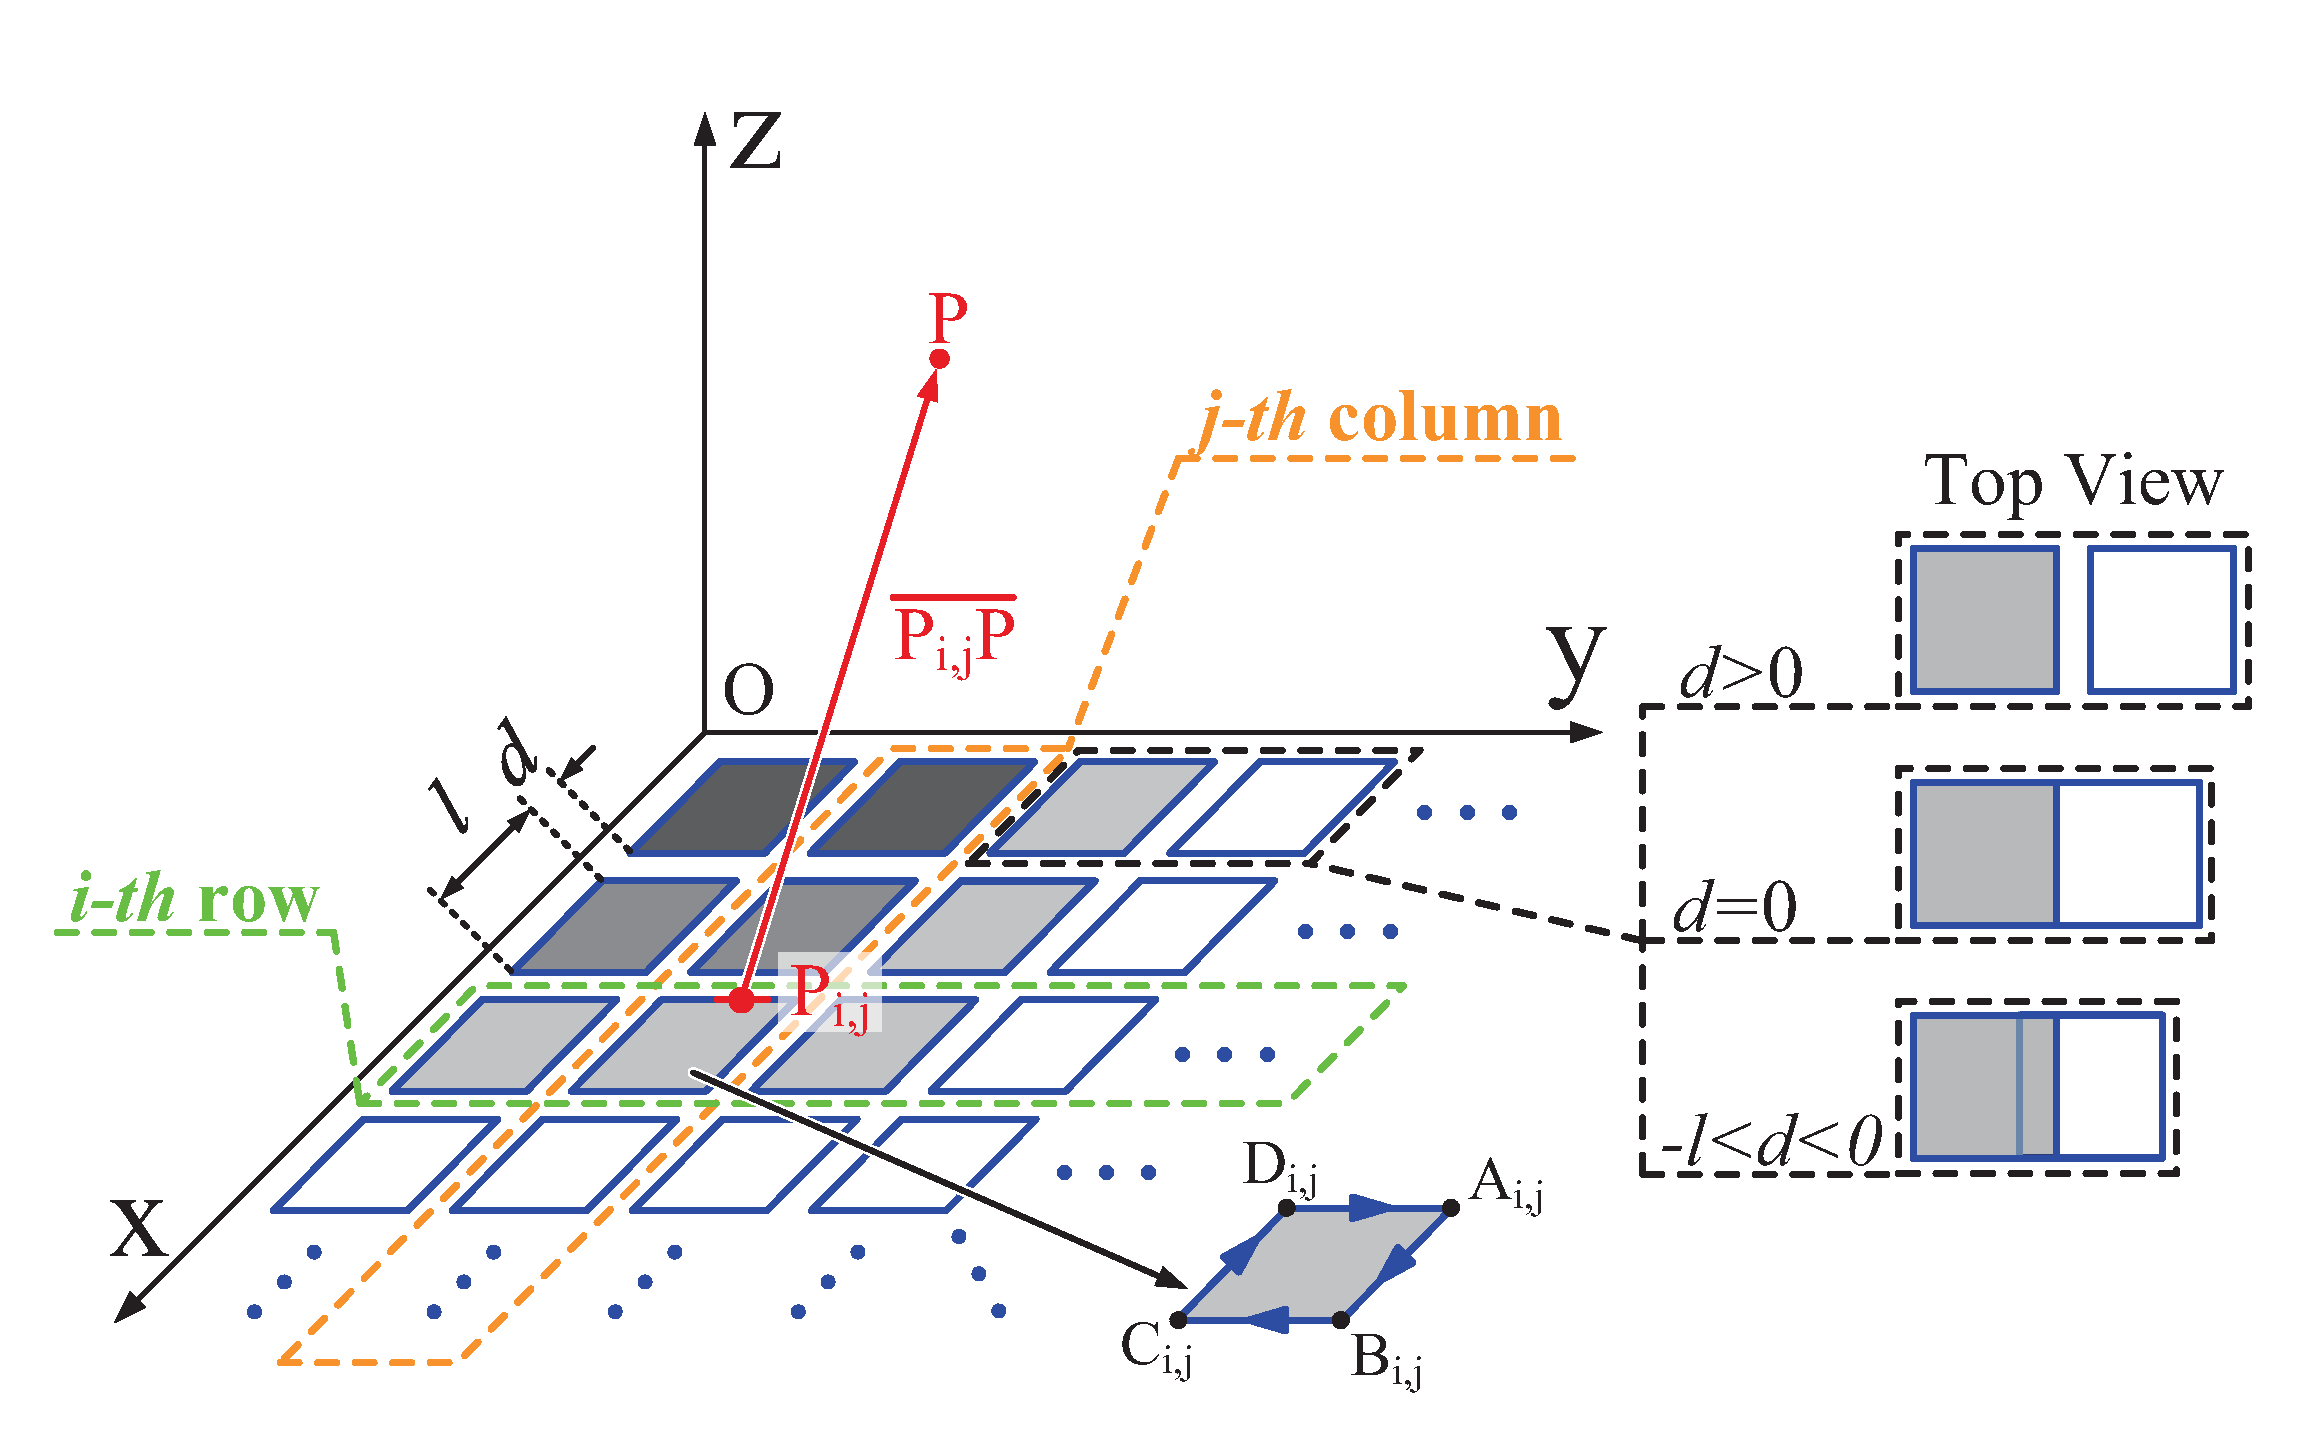
\includegraphics[width=8cm]{fig/fig1.eps}}
    \caption{An extendable planar Tx-coil array.}
    \label{fig:knij}
    %\vspace{-0.5cm}
\end{figure}
Therefore, this paper studies an extendable planar Tx-coil array architecture for the magnetic field shaping, which has a potential to charge devices with different 3D positions and orientations. First, the B-field distribution is analytically modelled in Section~\ref{sec:arch} to clarify the mechanism of the 3D magnetic field shaping through the 2D planar Tx-coil array. Secondly, the cross coupling between two adjacent Tx coils is especially analyzed, which is the unique challenge of adopting the planar array architecture, and is minimized later by optimally designing the layout of the Tx coils, as discussed in Section~\ref{sec:cross}. This reduces the interference among the Tx coils (i.e., additional reflected impedances) and thus helps to improve the operating conditions of power amplifiers (PAs) and the performance of the final WPT system. In section~\ref{sec:shaping}, calculation results of the B-field amplitude distribution are visualized to verify magnetic field shaping effects through the planar Tx-coil array and phase shift modulation of Tx-coil currents. Finally, Section~\ref{sec:exp} explains a complete experimental 6.78~MHz WPT system, implementing a 2$\times$2 planar Tx-coil array. An LED array is fabricated to experimentally visualize the actual magnetic field shaping and verify the consistency with the calculation results. The efficiency and output power are then measured and compared when transferring power to an Rx coil moving in six degrees of freedom. The results show significant improvements through the Tx-coil array-based magnetic shaping and minimized cross coupling design. In Section~\ref{sec:conclusion}, conclusions and main future works are addressed.

%\vspace{-0.5cm}
\section{Architecture and Modeling}
\label{sec:arch}

\subsection{Extendable Planar Tx-coil Array}
%\vspace{-0.5cm}
\begin{figure}[b!]
	\vspace{-0.8cm}
    \centering
    \centerline{\includegraphics[width=7.5cm]{fig/fig2.eps}}
    \caption{Typical system configuration.}
    \vspace{-0.3cm}
    \label{fig:PAarray}
\end{figure}
\begin{figure}[b!]
  \vspace{-0.3cm}
    \centering
    \subfigure[]{
    \label{t1}
    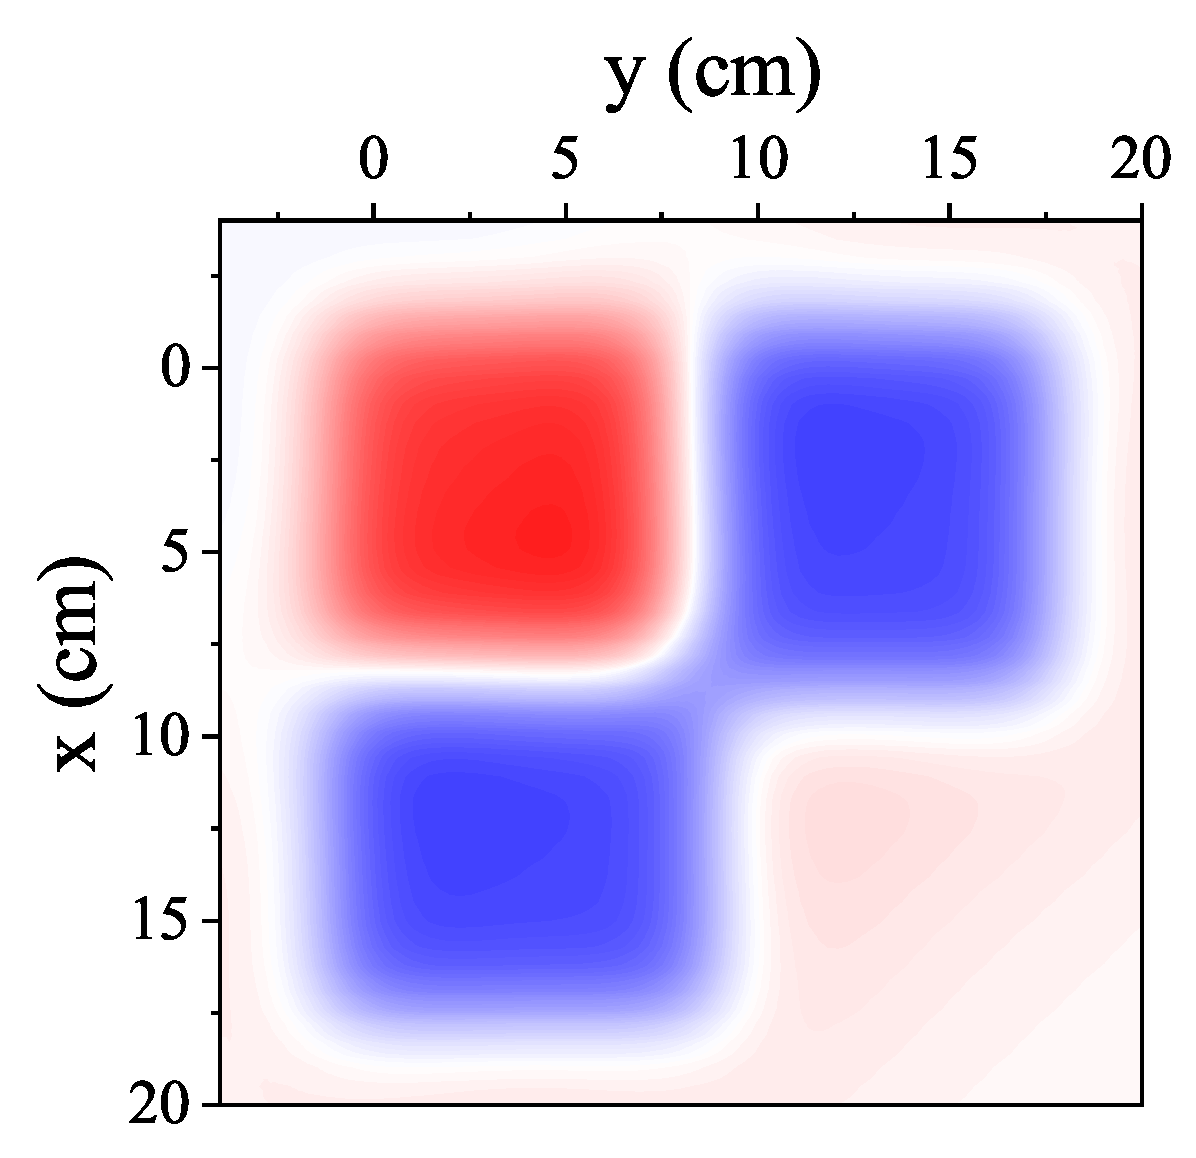
\includegraphics[height=3.5cm]{fig/fig3a.eps}}
    \subfigure[]{
    \label{t2}
    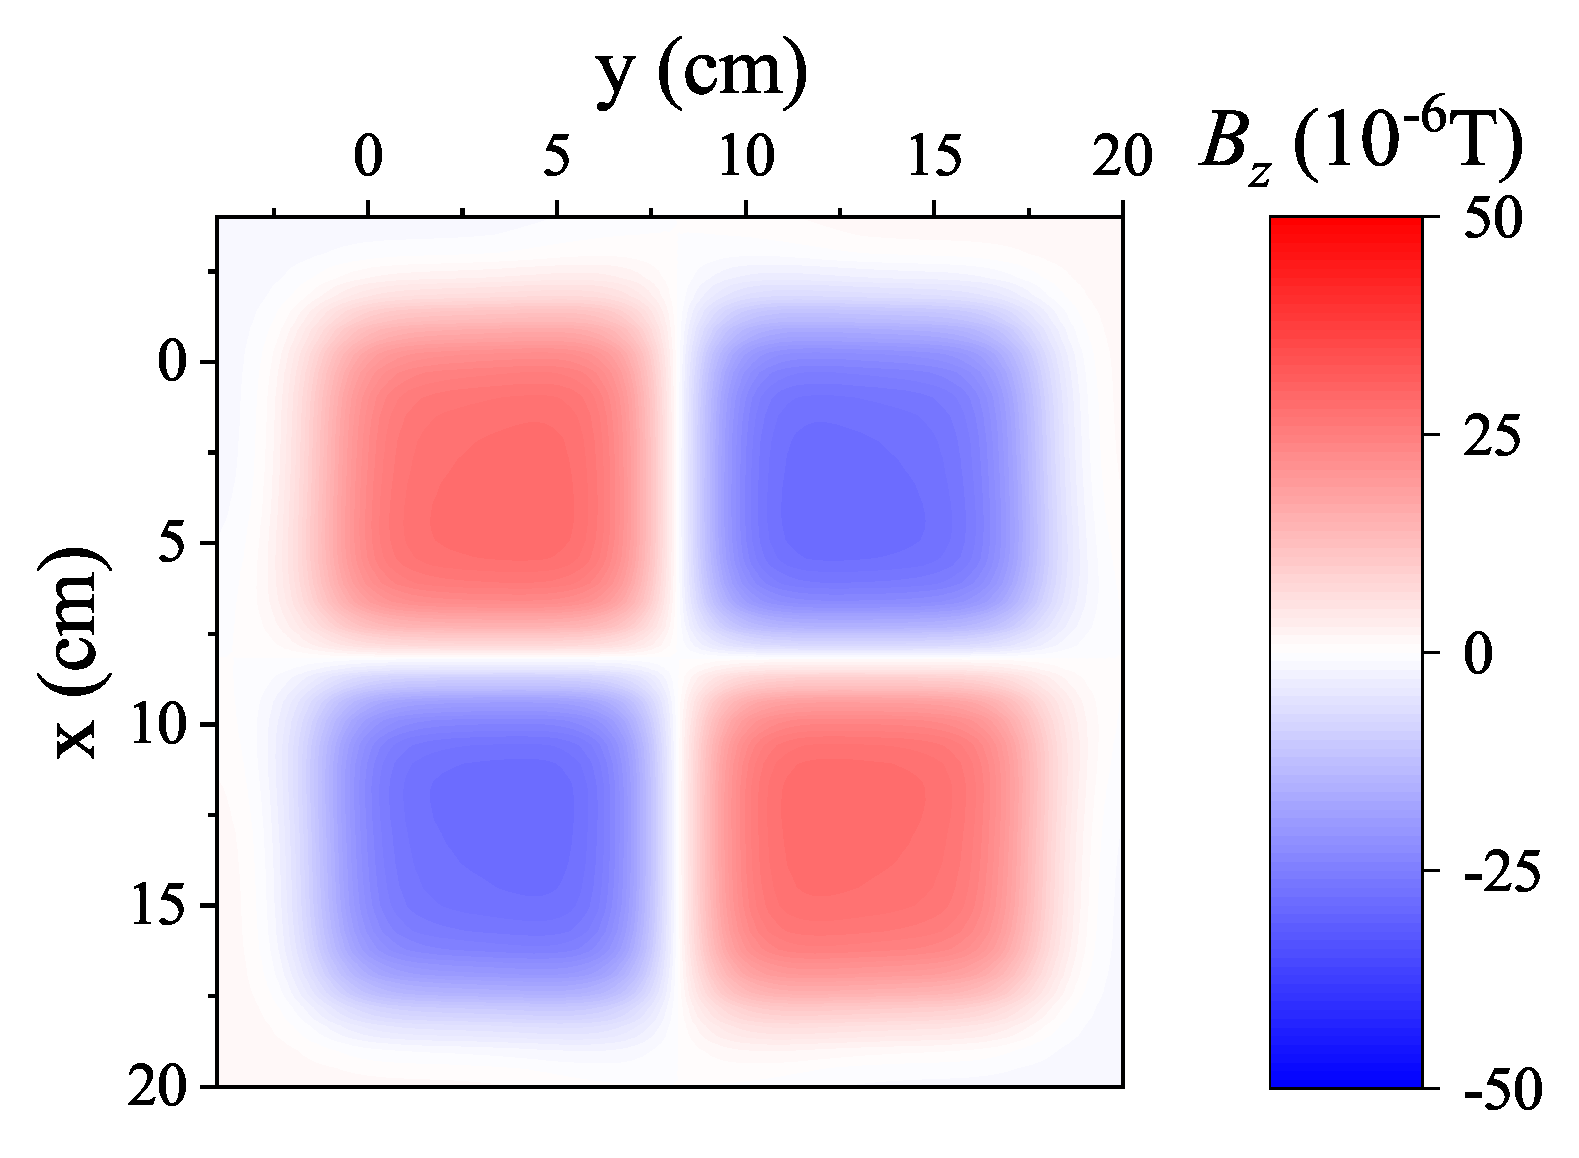
\includegraphics[height=3.53cm]{fig/fig3b.eps}}\\
    \subfigure[]{
    \label{t3}
    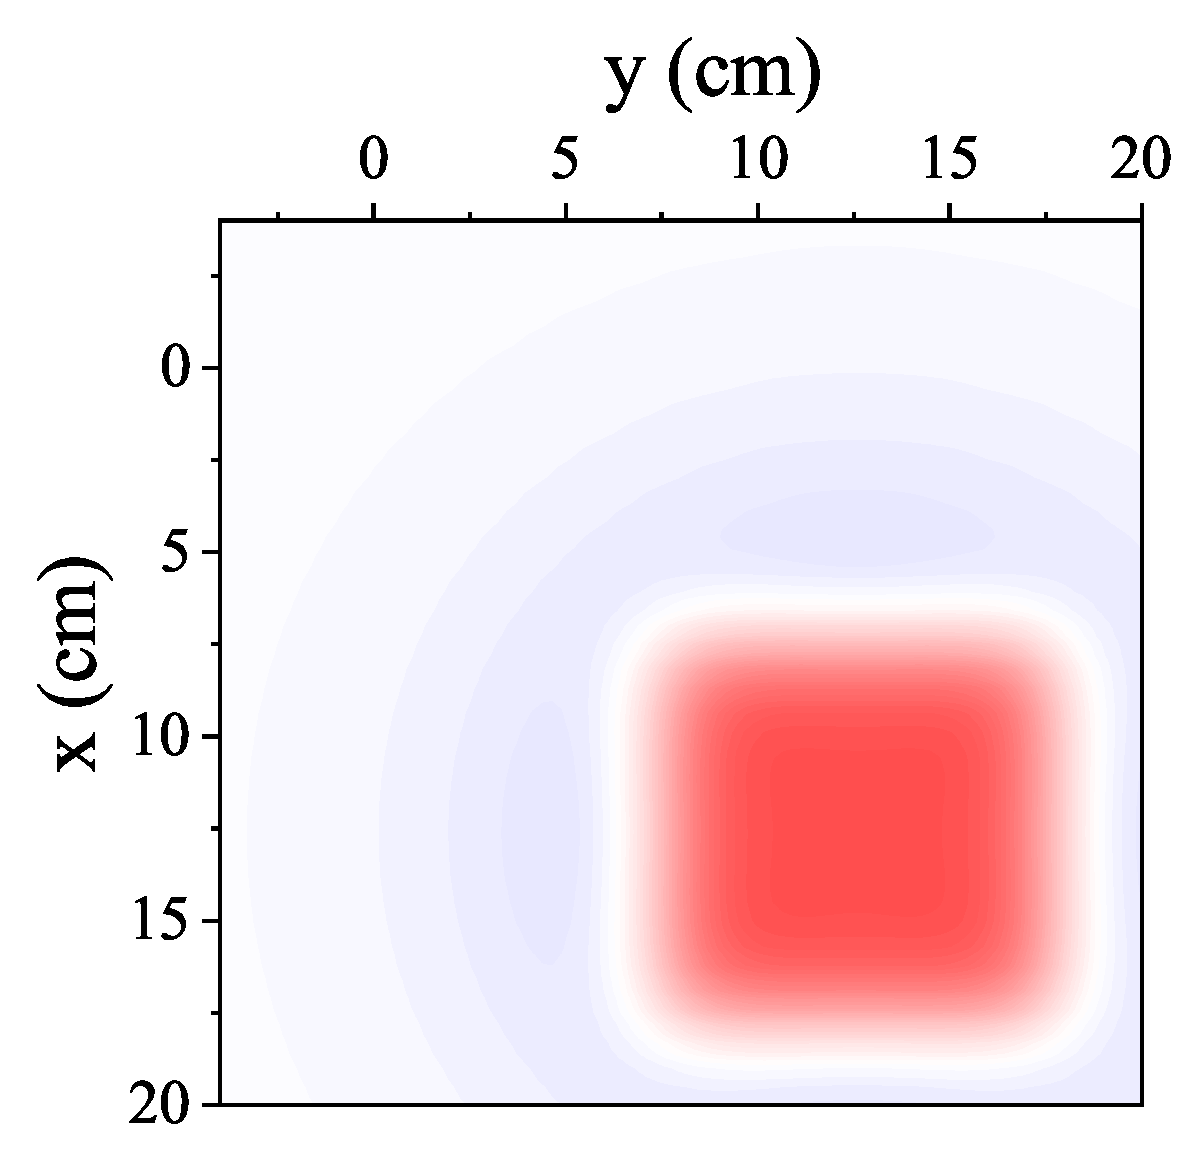
\includegraphics[height=3.5cm]{fig/fig3c.eps}}
    \subfigure[]{
    \label{t4}
    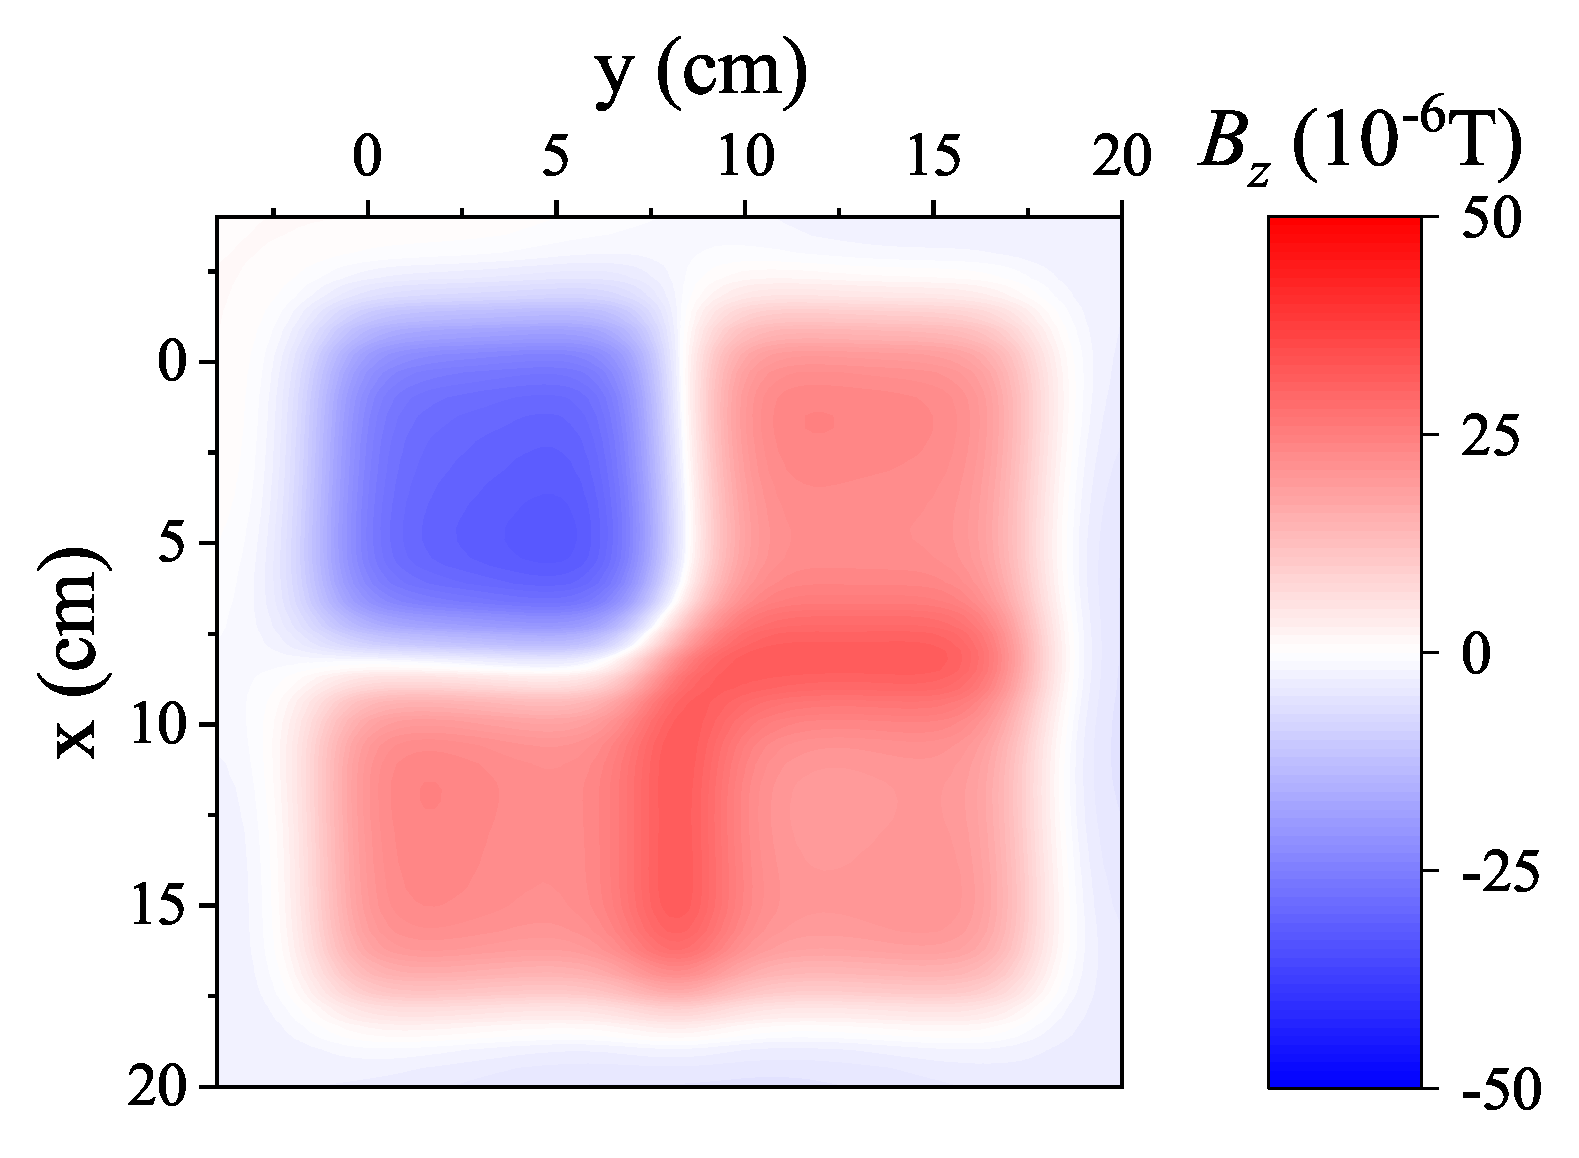
\includegraphics[height=3.53cm]{fig/fig3d.eps}}
    \caption{Calculation results of $z$-direction B-field generated by a $2 \times 2$ Tx-coil array at different observation time $t$ ($z=2.5~cm)$. (a) $\omega t=0$. (b) $\omega t = \frac{\mathrm{\pi}}{4}$. (c) $\omega t = \frac{\mathrm{\pi}}{2}$. (d) $\omega t = \frac{\mathrm{3\pi}}{4}$.}
    \label{fig:Biot}
\end{figure}
Fig.~\ref{fig:knij} illustrates the layout of an extendable planar Tx-coil array, such as using square coils. And Fig.~\ref{fig:PAarray} shows the relationship between PAs and Tx coils. Due to its 2D structure, modulating the phase shift in all the Tx coils is especially effective to shape the final magnetic field in 3D space. In the figure, the side length of each square coil is represented by $l$. Cross coupling between individual Tx coils changes with the distance $d$ between adjacent coils. In this planar coil array, all the Tx coils locate on the XOY plane, and the four corners of a single Tx-coil (${\rm Tx}_{i,j}$) in the $i$-th row and $j$-th column are:
	\begin{align}
		\begin{cases}
			\mathrm{A}_{i,j}\,\,\left( id+il-l, jd+jl, 0 \right) ,\\
			\mathrm{B}_{i,j}\,\,\left( id+il, jd+jl, 0 \right) ,\\
			\mathrm{C}_{i,j}\,\,\left( id+il, jd+jl-l, 0 \right) ,\\
			\mathrm{D}_{i,j}\,\,\left( id+il-l, jd+jl-l, 0 \right) .\\
		\end{cases}
		\label{points}
	\end{align}
And it is supposed that the current $I_{i,j}$ of Tx$_{i,j}$ flows from $\mathrm{A}_{i,j}$ to $\mathrm{B}_{i,j}$, $\mathrm{C}_{i,j}$ and $\mathrm{D}_{i,j}$.

\begin{figure*}[b]%\small
\hrulefill
\begin{align}\tag{8}
    \left[
      \begin{array}{c}
      B_{x}^m \\
      %\\
      B_{y}^m \\
      %\\
      B_{z}^m \\
      %\\
    \end{array}
  \right]
  =
  \left[
      \begin{array}{c}
      \left\{\left[\sum\limits _{i=1}^m \sum\limits _{j=1}^n B_{x}^m|_{i,j} \cos \left( \theta _{i,j}\right)\right]^2+
      \left[\sum\limits _{i=1}^m \sum\limits _{j=1}^n B_{x}^m|_{i,j} \sin \left( \theta _{i,j}\right)\right]^2\right\}^{\frac{1}{2}} \\
      \left\{\left[\sum\limits _{i=1}^m \sum\limits _{j=1}^n B_{y}^m|_{i,j} \cos \left( \theta _{i,j}\right)\right]^2+
      \left[\sum\limits _{i=1}^m \sum\limits _{j=1}^n B_{y}^m|_{i,j} \sin \left( \theta _{i,j}\right)\right]^2\right\}^{\frac{1}{2}} \\
      \left\{\left[\sum\limits _{i=1}^m \sum\limits _{j=1}^n B_{z}^m|_{i,j} \cos \left( \theta _{i,j}\right)\right]^2+
      \left[\sum\limits _{i=1}^m \sum\limits _{j=1}^n B_{z}^m|_{i,j} \sin \left( \theta _{i,j}\right)\right]^2\right\}^{\frac{1}{2}} \\
    \end{array}
  \right]
  \label{Bm}
\end{align}
%\hrulefill
\end{figure*}

In Fig.~\ref{fig:knij}, point ${\rm P}_{i,j}(x_{i,j},y_{i,j},z_{i,j})$ is on the Tx$_{i,j}$ and an arbitrary point P$(x,y,z)$ is in 3D space. A unity vector from ${\rm P}_{i,j}$ to P is $\hat{r}_{i,j}$, which can be expressed as
	\begin{align}
  		\nonumber \hat{r}_{i,j}&=\frac{\overline{\mathrm{P}_{i,j}\mathrm{P}}}{\left| \overline{\mathrm{P}_{i,j}\mathrm{P}} \right|}
  		\\
              			 	   &=\frac{\hat{e}_x\left( x-x_{i,j} \right) +\hat{e}_y\left( y-y_{i,j} \right) +\hat{e}_z\left( z-z_{i,j} \right)}{\sqrt{\left( x-x_{i,j} \right) ^2+\left( y-y_{i,j} \right) ^2+\left( z-z_{i,j} \right) ^2}},
    \label{univector}
	\end{align}
where $\hat{e}_x$, $\hat{e}_y$ and $\hat{e}_z$ are unity vectors in $x$, $y$ and $z$ directions. The current $I_{i,j}$ in ${\rm Tx}_{i,j}$ is
\begin{align}
		I_{i,j} = I_{i,j}^m \cos \left(\omega t+\theta _{i,j}\right),
		\label{current}
\end{align}
where $I_{i,j}^m$ is amplitude, $\theta _{i,j}$ is initial phase, and $\omega$ is a target operating frequency, such as 6.78~MHz in this paper. Based on the Biot-Savart law and \eqref{points}--\eqref{current}, the magnetic flux density induced by Tx$_{i,j}$ at an arbitrary point P can be derived as
\begin{align}
  %\nonumber \mathbf
  \nonumber & \overline{B _{i,j}} =\oint \frac{\mu _0}{4 \pi } \frac{N_{tx} I_{i,j}^{m} \cos \left( \omega t +\theta _{i,j} \right) \overline{dl} \times \hat{r}_{i,j}}{r_{i,j}^2}
  \\
  \nonumber &= \frac{\mu _0 N_{tx} I_{i,j}^{m} \cos \left(\omega t + \theta_{i,j} \right)}{4 \pi } \cdot
  \\
  \hspace{-1cm} \nonumber & \left\{ \int _{\mathrm{A}_{\mathrm{i},\mathrm{j}}\mathrm{B}_{\mathrm{i},\mathrm{j}}}\frac{1}{r_{i,j}^3}\left[ \hat{e}_z \left(y-y_{i,j}\right) dx- \hat{e}_y \left(z-z_{i,j}\right)dx\right]\right.
  \\
  \nonumber & -\int _{\mathrm{B}_{\mathrm{i},\mathrm{j}}\mathrm{C}_{\mathrm{i},\mathrm{j}}}\frac{1}{r_{i,j}^3}\left[ \hat{e}_x \left(z-z_{i,j}\right)dy-\hat{e}_z \left(x-x_{i,j}\right)dy\right]
  \\
  \nonumber & -\int _{\mathrm{C}_{\mathrm{i},\mathrm{j}}\mathrm{D}_{\mathrm{i},\mathrm{j}}}\frac{1}{r_{i,j}^3}\left[ \hat{e}_z \left(y-y_{i,j}\right)dx-\hat{e}_y \left(z-z_{i,j}\right)dx\right]
  \\
            & \left.+\int _{\mathrm{D}_{\mathrm{i},\mathrm{j}}\mathrm{A}_{\mathrm{i},\mathrm{j}}}\frac{1}{r_{i,j}^3}\left[ \hat{e}_x \left(z-z_{i,j}\right)d y- \hat{e}_z \left(x-x_{i,j}\right)dy \right]\right\},
    \label{Bijmid}
\end{align}
where $N_{tx}$ is the number of turns of Tx$_{i,j}$; $\mu _0$ is the permeability of vacuum. Note that $\overline{B _{i,j}}$ has its $B_x|_{i,j}$, $B_y|_{i,j}$ and $B_z|_{i,j}$ terms. Detailed derivations of $B_x|_{i,j}$, $B_y|_{i,j}$ and $B_z|_{i,j}$ are listed in the Appendix. The B-field at point P is the sum of the B-field induced by each coil in an $m \times n$ Tx-coils array,
\begin{align}
    \left[
    	\begin{array}{c}
 			B_x \\
 			B_y \\
 			B_z \\
		\end{array}
	\right]
	=
	\left[
    	\begin{array}{c}
 			\sum\limits _{i=1}^m \sum\limits _{j=1}^n B_x|_{i,j} \\
 			\sum\limits _{i=1}^m \sum\limits _{j=1}^n B_y|_{i,j} \\
 			\sum\limits _{i=1}^m \sum\limits _{j=1}^n B_z|_{i,j} \\
		\end{array}
	\right].
	\label{totalBt}
\end{align}

As shown by the calculation results in Fig.~\ref{fig:Biot}, the $z$-direction B-field induced by a 2$\times$2 coil array, as an example, changes with time. The four coils, namely Tx$_{1,1}$, Tx$_{1,2}$, Tx$_{2,1}$ and Tx$_{2,2}$, have the same current amplitude and frequency, while the phases of the four coils are $180^{\circ}$, $0^{\circ}$, $0^{\circ}$, and $90^{\circ}$, respectively. The real-time B-field strength at the same position changes with time, but its amplitude is fixed and corresponds to the maximum receiving power.

\subsection{B-field Amplitude Distribution Function}
To obtain the B-field Amplitude Distribution Function~(ADF), the expression of the B-field can be first simplified as follows:
\begin{align}
    \left[
    	\begin{array}{c}
 			B_x \\
 			B_y \\
 			B_z \\
		\end{array}
	\right]
	=
	\left[
    	\begin{array}{c}
 			B_{x}^m \cos  \left(\omega t+\theta _{x}\right) \\
 			B_{y}^m \cos  \left(\omega t+\theta _{y}\right) \\
 			B_{z}^m \cos  \left(\omega t+\theta _{z}\right) \\
		\end{array}
	\right],
\end{align}
where $B_{x}^m$, $B_{y}^m$ and $B_{z}^m$ are the ADFs of $x$-direction, $y$-direction, and $z$-direction components of the B-field; $\theta _{x}$, $\theta _{y}$ and $\theta _{z}$ are the initial phases. The phasor representation of the B-field at point P is
\begin{align}
    \left[
    	\begin{array}{c}
 			{\bf B}_x \\
 			{\bf B}_y \\
 			{\bf B}_z \\
		\end{array}
	\right]
	=
	\left[
    	\begin{array}{c}
 			\frac{B_{x}^m}{\sqrt{2}} \phase{\theta _{x}}    \\
 			\frac{B_{y}^m}{\sqrt{2}} \phase{\theta _{y}}    \\
 			\frac{B_{z}^m}{\sqrt{2}} \phase{\theta _{z}}    \\
		\end{array}
	\right]
	=
	\left[
    	\begin{array}{c}
 			\sum\limits _{i=1}^m \sum\limits _{j=1}^n {\bf B}_x|_{i,j} \\
 			\sum\limits _{i=1}^m \sum\limits _{j=1}^n {\bf B}_y|_{i,j} \\
 			\sum\limits _{i=1}^m \sum\limits _{j=1}^n {\bf B}_z|_{i,j} \\
		\end{array}
	\right].
\end{align}

The B-field ADFs in three directions are calculated and give in~\eqref{Bm} at the bottom of this page. As shown in the three equations, $B_{x}^m$, $B_{y}^m$, and $B_{z}^m$ are jointly determined by the ADFs $B_{\left\{ \bullet \right\}}^m|_{i,j}$ and initial phase $\theta _{i,j}$ of all the individual Tx coils. It should be noted that \eqref{Bm} has no time-related variables. This advantage makes it convenient to check the B-field strength in different 3D positions and thus the actual magnetic field shaping effect~[see Figs.~\ref{3deg1} and \ref{3deg2} in Section~\ref{sec:shaping}].

  \begin{figure}[ht!]
  	  \vspace{-0.3cm}
      \centering
      \centerline{\includegraphics[width=8.5cm]{fig/fig4.eps}}
      \caption{Two types of cross coupling in a planar Tx-coil array.}
      \vspace{-0.3cm}
      \label{2couping}
  \end{figure}
\section{Cross Coupling and Its Minimization}
\label{sec:cross}

\subsection{Analysis and Modeling}
In the planar Tx-coil array, each Tx coil may actually act as an Rx coil to other Tx coils when these coils are crossly coupled. This unique nature, i.e., the cross coupling between the Tx coils, may
\begin{enumerate}
  \item reduce the power that is supposed to be fed into the receiver, which is certainly unfavorable for overall system performance such as efficiency~\cite{feng2019transmitter};

  \item impact and complicate the operation of PAs because the cross coupling makes each PA see the impedance reflected by other transmitters. This reflected impedance may also significantly change with different phases of the coil currents~\cite{feng2020lccl}.

  \item pose a severe challenge to effective shaping of the final magnetic field~\cite{zhu2017field}.
\end{enumerate}
As discussed in next subsection, this cross coupling between the Tx-coils can be properly managed by designing the distance $d$ between the Tx coils~[see Fig.~\ref{fig:knij}].

\begin{figure*}[hb!]
    \centering
    \vspace{-0.3cm}
    \subfigure[]{
    \label{k1}
    \includegraphics[width=5.6cm]{fig/fig5a.eps}}
    \subfigure[]{
    \label{k2}
    \includegraphics[width=5.6cm]{fig/fig5b.eps}}\
    \subfigure[]{
    \label{k22}
    \includegraphics[width=5.6cm]{fig/fig5c.eps}}
    \caption{Cross coupling coefficients $k_1$ and $k_2$ versus Tx-coil distance $d$ (coil length $l=$9~cm). (a) $k_1$. (b) $k_2$. (c) $k_1$, $k_2$ and $k_{avg}$ in a 2$\times$2 Tx-coil array.}
    \label{k}
\end{figure*}

Fig.~\ref{2couping} shows two types of cross coupling in a planar Tx-coil array. $k_1$ is defined to represent the cross coupling coefficient between two adjacent coils in the same row or column (e.g., gray and orange coils), while $k_2$ represents the cross coupling coefficient between two adjacent coils in next different row and column (e.g., gray and green coils). Note that only cross-coupling of adjacent coils is considered because the cross-coupling between other Tx coils is usually negligible~\cite{fu2015efficiency}. Based on Fig.~\ref{2couping}, the mutual inductances of the two types of Tx-coil pairs, $M_1$ and $M_2$, are
\begin{align}\tag{9}
  \frac{\Phi _{i,j-1}}{I_{i,j}}=\frac{\Phi _{i,j+1}}{I_{i,j}}=\frac{\Phi _{i-1,j}}{I_{i,j}}=\frac{\Phi _{i+1,j}}{I_{i,j}}=M_1,
  \label{M1}
\end{align}
\begin{align}\tag{10}
  \frac{\Phi _{i-1,j-1}}{I_{i,j}}=\frac{\Phi _{i+1,j-1}}{I_{i,j}}=\frac{\Phi _{i-1,j+1}}{I_{i,j}}=\frac{\Phi _{i+1,j+1}}{I_{i,j}}=M_2,
  \label{M2}
\end{align}
where $I_{i,j}$ is the current of Tx$_{i,j}$, and $\Phi$'s are the flux linkages. For example, the flux linkage of Tx$_{i,j+1}$, namely $\Phi _{i,j+1}$, can be derived as [refer to Table~\ref{Bcomponents} in Appendix]
	\begin{align}\tag{11}
	  \Phi _{i,j+1}\left( {N_{tx},d},l \right) = N_{tx} \iint\limits_{S_{i,j+1}} \lim_{z\rightarrow 0} B_z|_{{i,j}} dx dy,
	\end{align}
where $N_{tx}$ is again coil turns and $S_{i,j+1}$ is coil area. For the sake of simplicity, here each coil is assumed to have the same area. Similarly, the maximum values of $M_1$ and $M_2$ can also be represented as
\begin{align}
  	\nonumber M_{1}^{\max}=M_{2}^{\max} &=\frac{\Phi _{i,j}\left( N_{tx},d,l \right)}{I_{i,j}}. \tag{12}
    \label{Mmax12}
\end{align}
From the above equations, the two cross coupling coefficients, $k_1$ and $k_2$, can be calculated as
	\begin{align} \tag{13}
	  k_1=\frac{M_1}{M_{1}^{\max}},~k_2=\frac{M_2}{M_{2}^{\max}}.
	  \label{k2cal}
	\end{align}

\subsection{Minimization via Overlap Design}
\label{sub:minimize}

Fig.~\ref{k1} shows the relationship between $k_1$ and $d$. The calculation results are in good agreement with the simulation results obtained by the High-Frequency Structure Simulator~(HFSS). Note that the coil model in HFSS is the same as the actual PCB model~[see Fig.~\ref{system}]. In calculation, the side length $l$ of the coils is 9~cm, which is equal to the average length of each turn in the simulation model. Interestingly, there is an overlap distance (i.e., a negative $d$) corresponding to the same amount of positive and negative magnetic field fluxes. This overlap distance largely decouples the two Tx coils, namely close-to-zero cross coupling. Similar results can be seen in Fig.~\ref{k2} too ($k_2$ versus $d$). It is because that based on the right-hand rule, the direction of the magnetic flux inside and outside a coil is opposite. Therefore, there exists an overlap area to cancel the cross coupling between adjacent Tx coils.

The two overlap distances that make $k_1$ and $k_2$ equal to zero are not the same. The sum of all cross-coupling coefficients ($k_1$'s and $k_2$'s) of the Tx-coil array ($m \times n$ coils) is
	\begin{align}\tag{14}
	  k_{\mathrm{sum}}=\left( 2 m n - m - n \right) k_1+2\left(m -1 \right) \left(n-1 \right) k_2.
	  \label{kt}
	\end{align}
Then, an average cross coupling coefficient can be defined to guide the design of $d$,
	\begin{align}\tag{15}
	  k_{\rm avg}=\frac{k_{\mathrm{sum}}}{4mn-3m-3n+2},
	  \label{ka}
	\end{align}
in which the denominator is the total number of the two types of cross coupling in the Tx-coil array. Fig.~\ref{k22} shows a comparison of $k_1$, $k_2$ and $k_{avg}$ in a 2$\times$2 Tx-coil array. The Tx-coil distance $d$ that minimizes $k_{avg}$ is close to the distance that minimizes $k_1$, because $k_1$ changes more drastically with $d$ than $k_2$.

\begin{figure}[t!]
    \centering
    \subfigure[]{
    \label{kd11}
    \includegraphics[width=4.22cm]{fig/fig6a.eps}}
    \subfigure[]{
    \label{kd22}
    \includegraphics[width=4.26cm]{fig/fig6b.eps}}\
    \caption{Cross coupling coefficients versus different $d$ and $l$. (a) $k_1$. (b) $k_2$.}
    \vspace{-0.3cm}
    \label{kd}
\end{figure}
 Fig.~\ref{kd11} and Fig.~\ref{kd22} show $k_1$ and $k_2$ under different $d$ and $l$. Despite slight differences, $d$'s that minimize $k_1$ and $k_2$ are almost in the same proportion as $l$'s. The optimal value of $d$ that minimizes the dominant $k_1$ can be further fine-tuned using detailed HFSS coil models, as shown in Fig.~\ref{fig:4para}(a). In the above calculation, the optimal $k_1$ is -1.11~cm~[see Fig.~\ref{k22}]. In all the cases in Fig.~\ref{fig:ntx}--(e), the average length of each turn $l$ is the same as that calculated above, i.e., 9~cm. As shown in these subfigures, the optimal $d$'s under different coil turns, trace width, and trace spacing are close with a maximum deviation of 0.2~cm. Note that Fig.~\ref{fig:f} shows that the optimal $d$'s under different operating frequencies ($f$) are identical. It is because $f$ does not impact the 3D magnetic field distribution; $f$ only affects the changing ratio of the magnetic field~[refer to Table~\ref{Bcomponents}]. Therefore, the optimal overlap design can be conducted through the combination of calculation and HFSS-based simulation:
 \begin{enumerate}
   \item calculate theoretically the optimal $d$ using \eqref{M1} -- \eqref{ka};
   \item further fine-tune and finalize the optimal $d$ using the detailed HFSS coil models.
 \end{enumerate}
\begin{figure}[ht!]
    \centering
    %\flushright
    \vspace{-0.3cm}
    \hspace{0.3cm}
    \subfigure[]{
    \label{fig:ugcoils}
    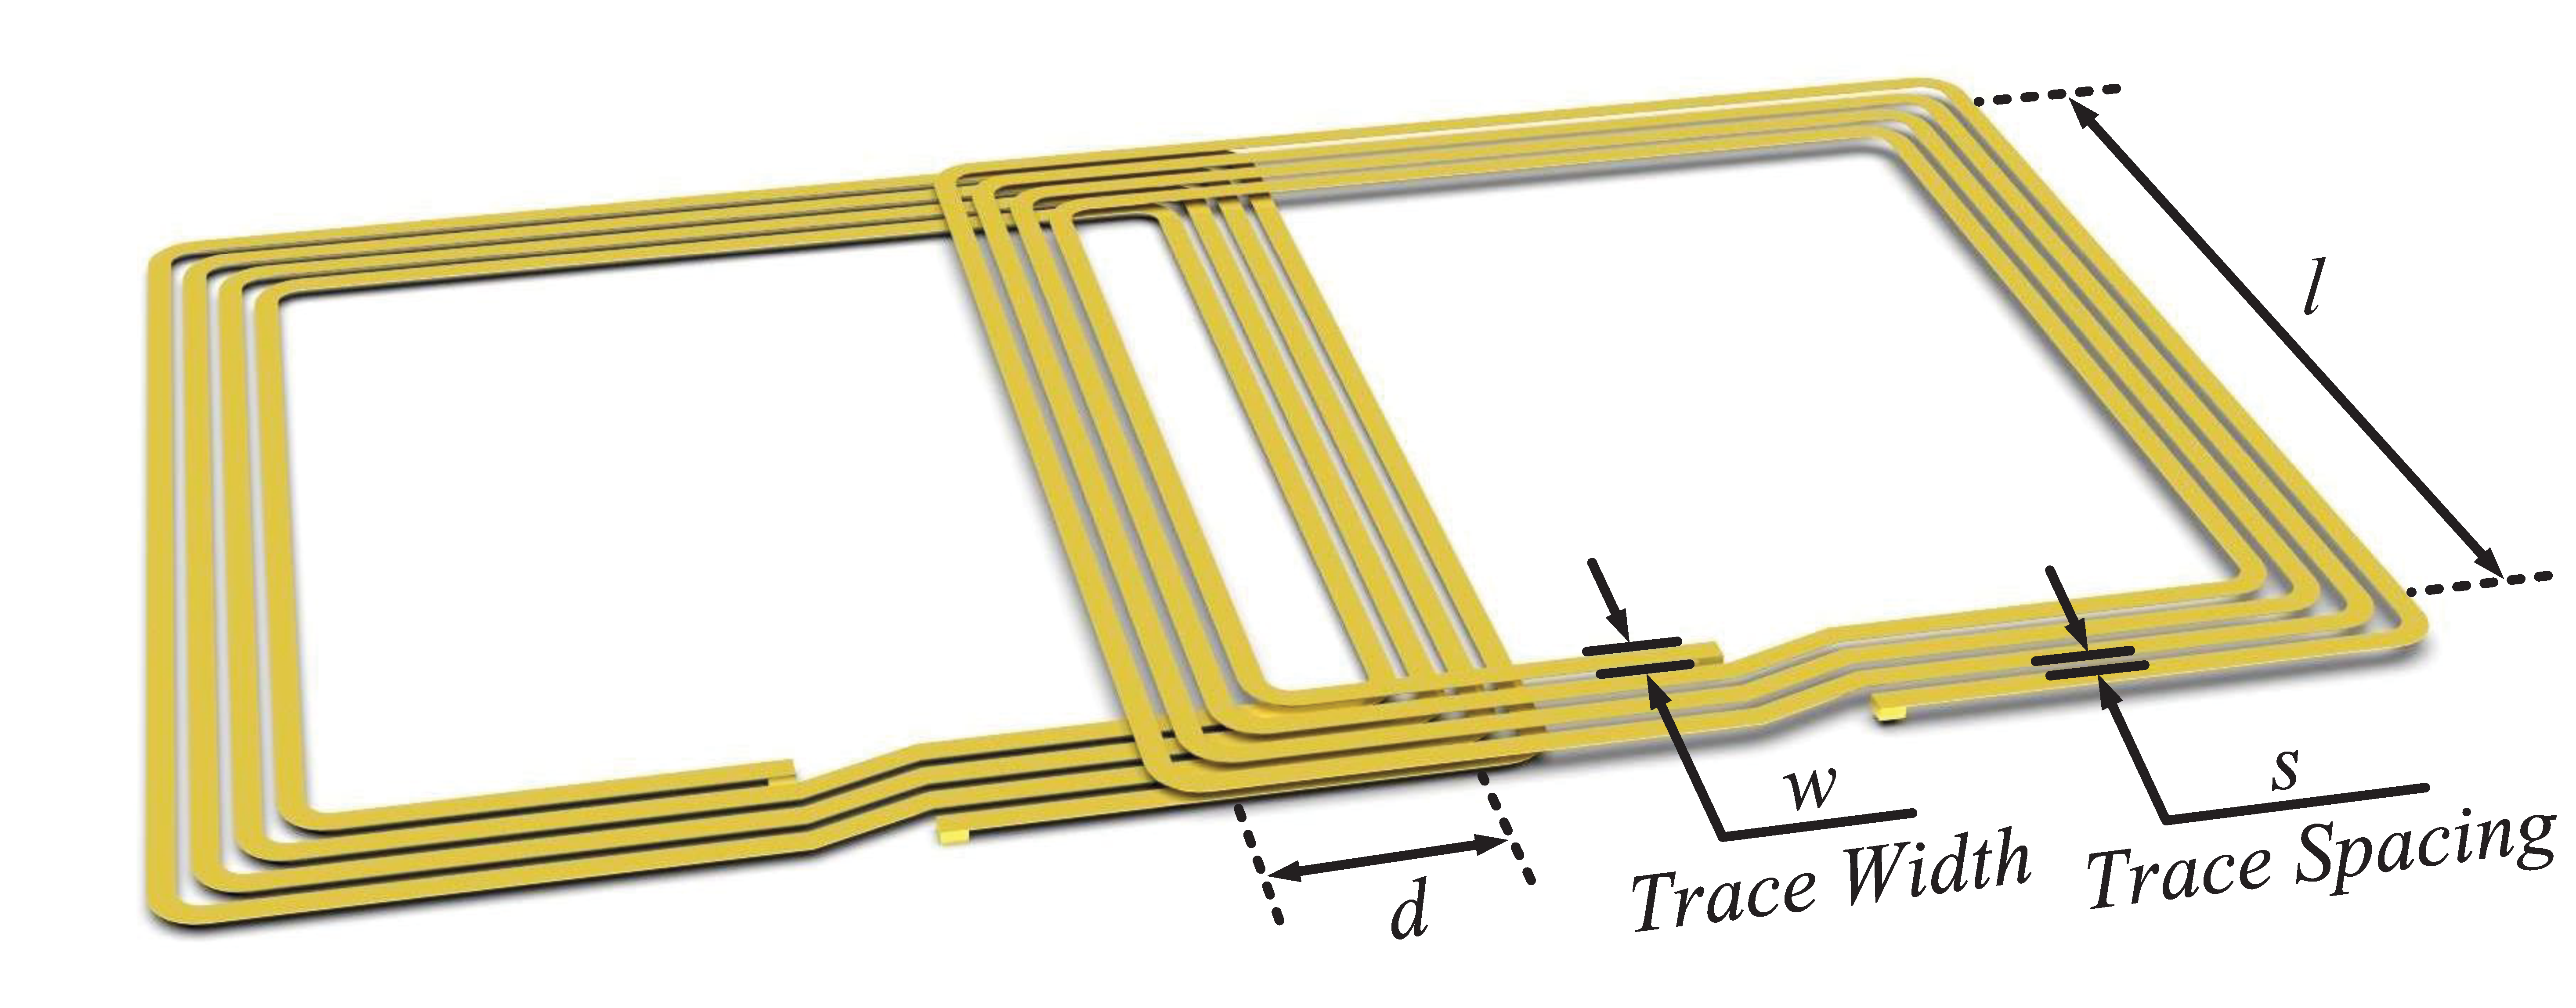
\includegraphics[width=6.5cm]{fig/fig7a.eps}}\\
    \subfigure[]{
    \label{fig:ntx}
    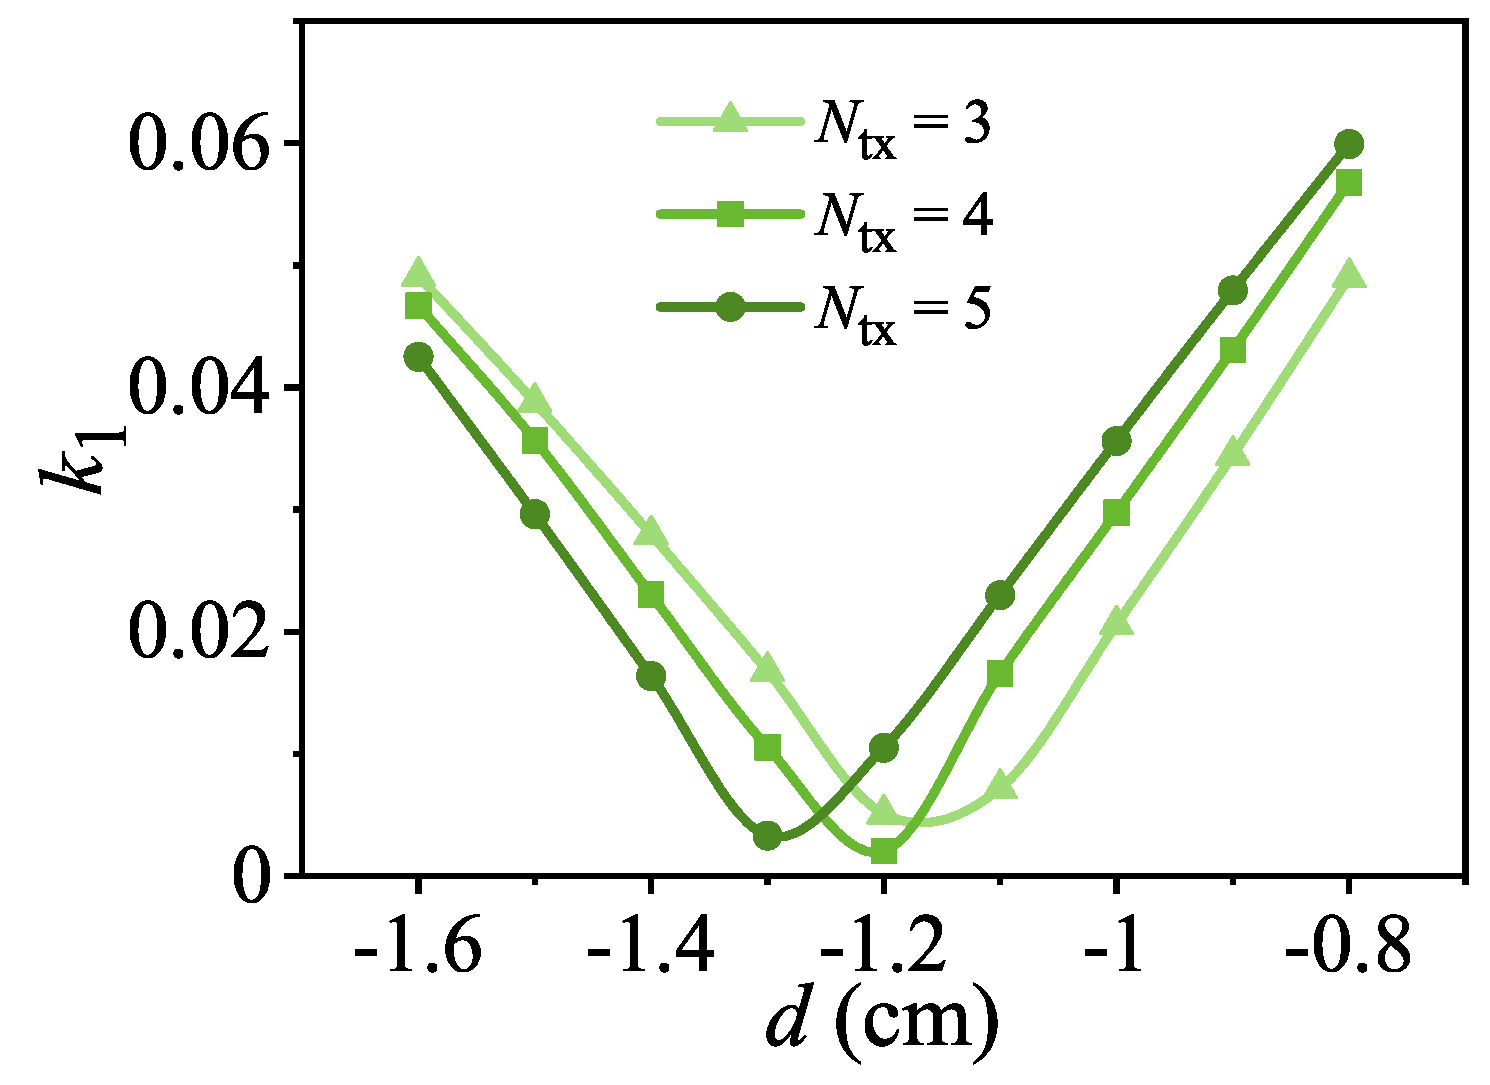
\includegraphics[width=4.22cm]{fig/fig7b.eps}}
    \subfigure[]{
    \label{fig:s}
    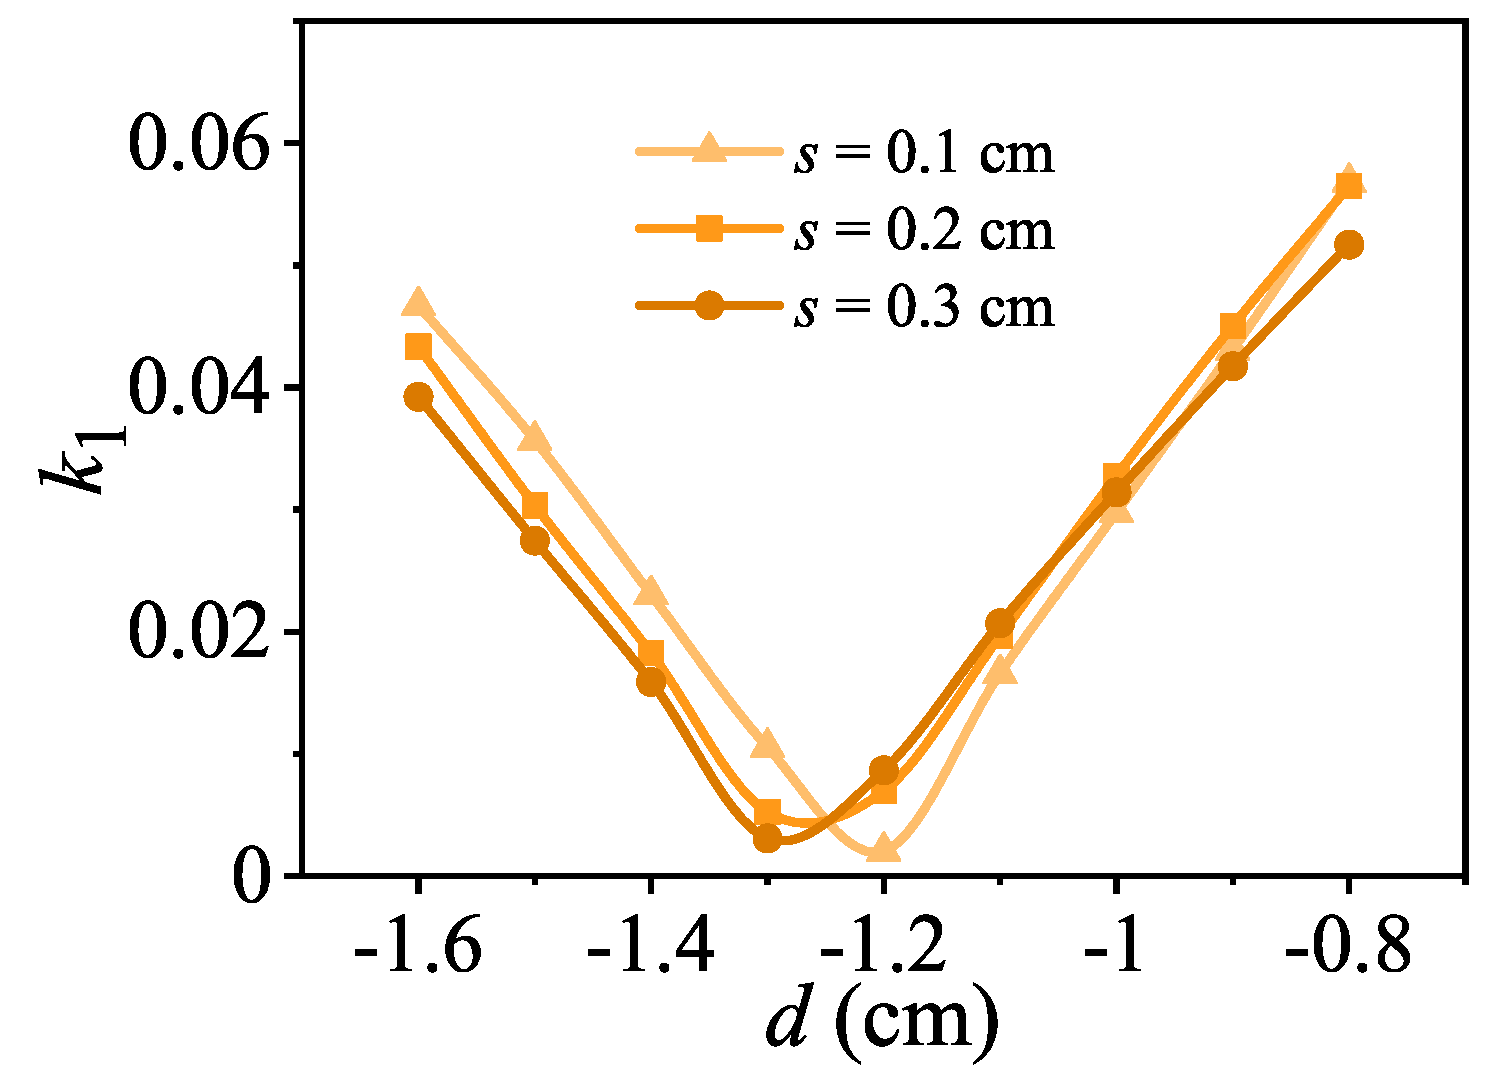
\includegraphics[width=4.22cm]{fig/fig7c.eps}}\\
    \subfigure[]{
    \label{fig:w}
    \includegraphics[width=4.22cm]{fig/fig7d.eps}}
    \subfigure[]{
    \label{fig:f}
    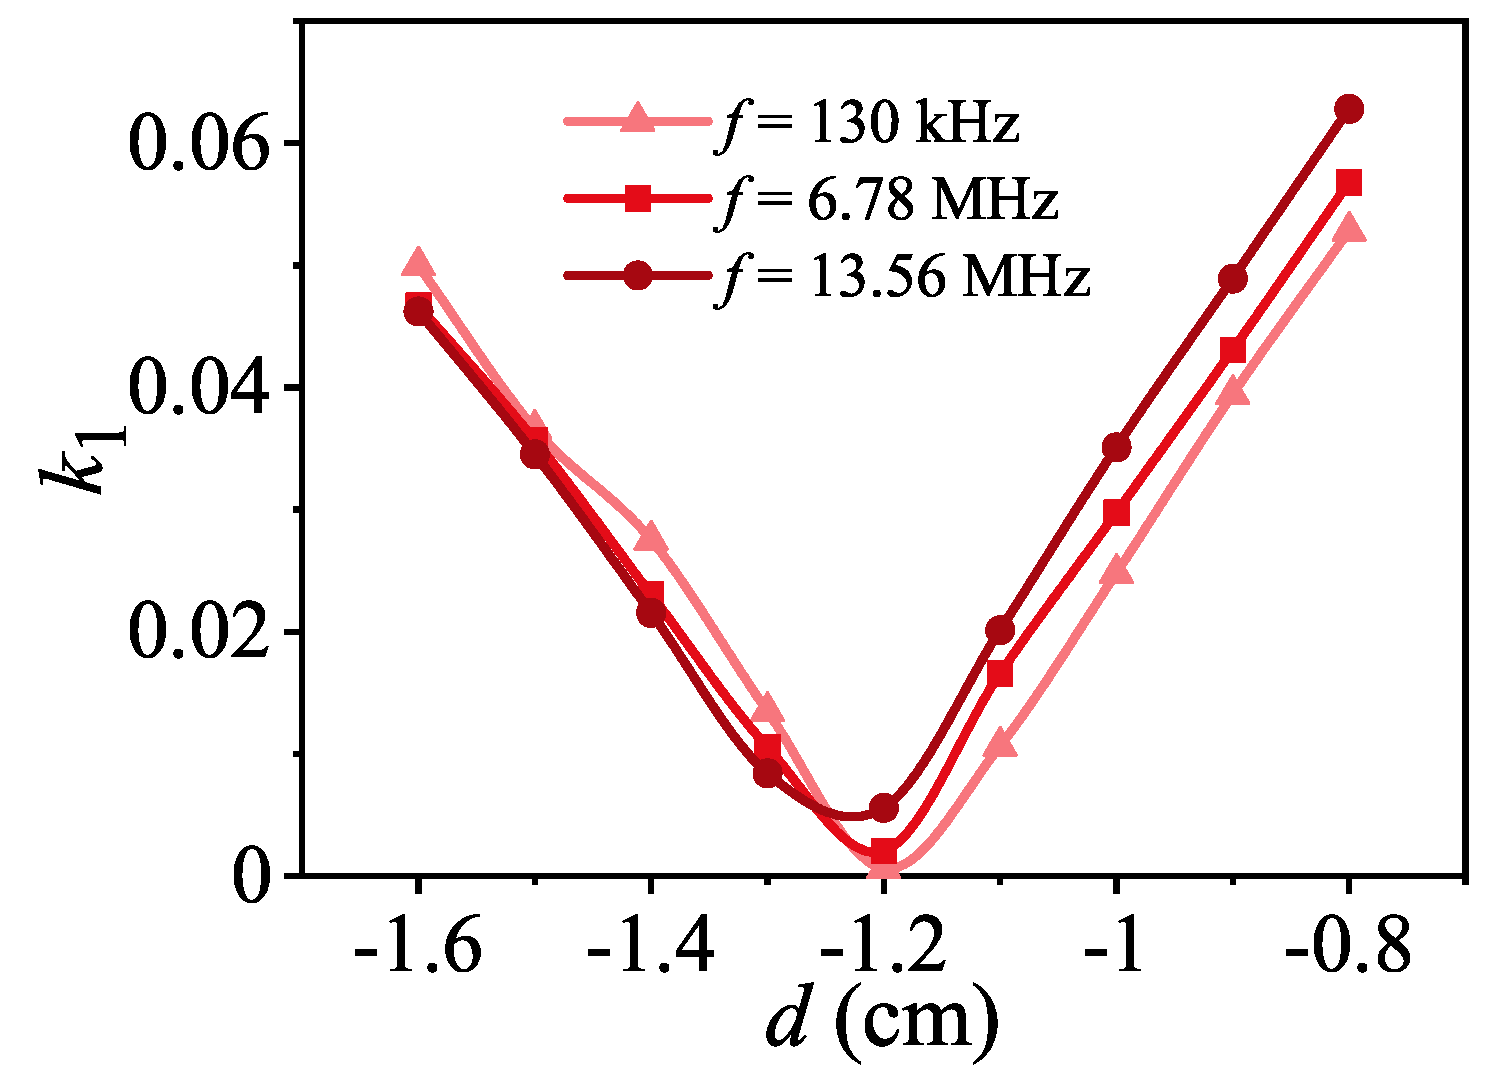
\includegraphics[width=4.22cm]{fig/fig7e.eps}}
    \caption{$k_1$ versus $d$ through the HFSS simulation.
    (a) Coil model.
    (b) Different $N_{\rm tx}$ ($l=9~\mathrm{cm}$, $s=0.1~\mathrm{cm}$, $w=0.2~\mathrm{cm}$, and $f=6.78~\mathrm{MHz}$).
    (c) Different $s$ ($l=9~\mathrm{cm}$, $N_{\rm tx}=4$, $w=0.2~\mathrm{cm}$, and $f=6.78~\mathrm{MHz}$).
    (d) Different $w$ ($l=9~\mathrm{cm}$, $N_{\rm tx}=4$, $s=0.1~\mathrm{cm}$, and $f=6.78~\mathrm{MHz}$).
    (e) Different $f$ ($l=9~\mathrm{cm}$, $N_{\rm tx}=4$, $s=0.1~\mathrm{cm}$, and $w=0.2~\mathrm{cm}$).}
    \label{fig:4para}
\end{figure}

For reference purposes, the relationship between overlap distance $d_{\rm s}$ and cross coupling coefficient $k_{\rm s}$ is also investigated for spiral coils, as shown in Fig.~\ref{fig:scoils}. A similar trend can be observed, and there is a specific $d_{\rm s}$ to respectively minimize the cross coupling in both pairs of spiral coils.
\begin{figure}[t!]
    \centering
    \vspace{-0.3cm}
    \subfigure[]{
    \label{fig:s4}
    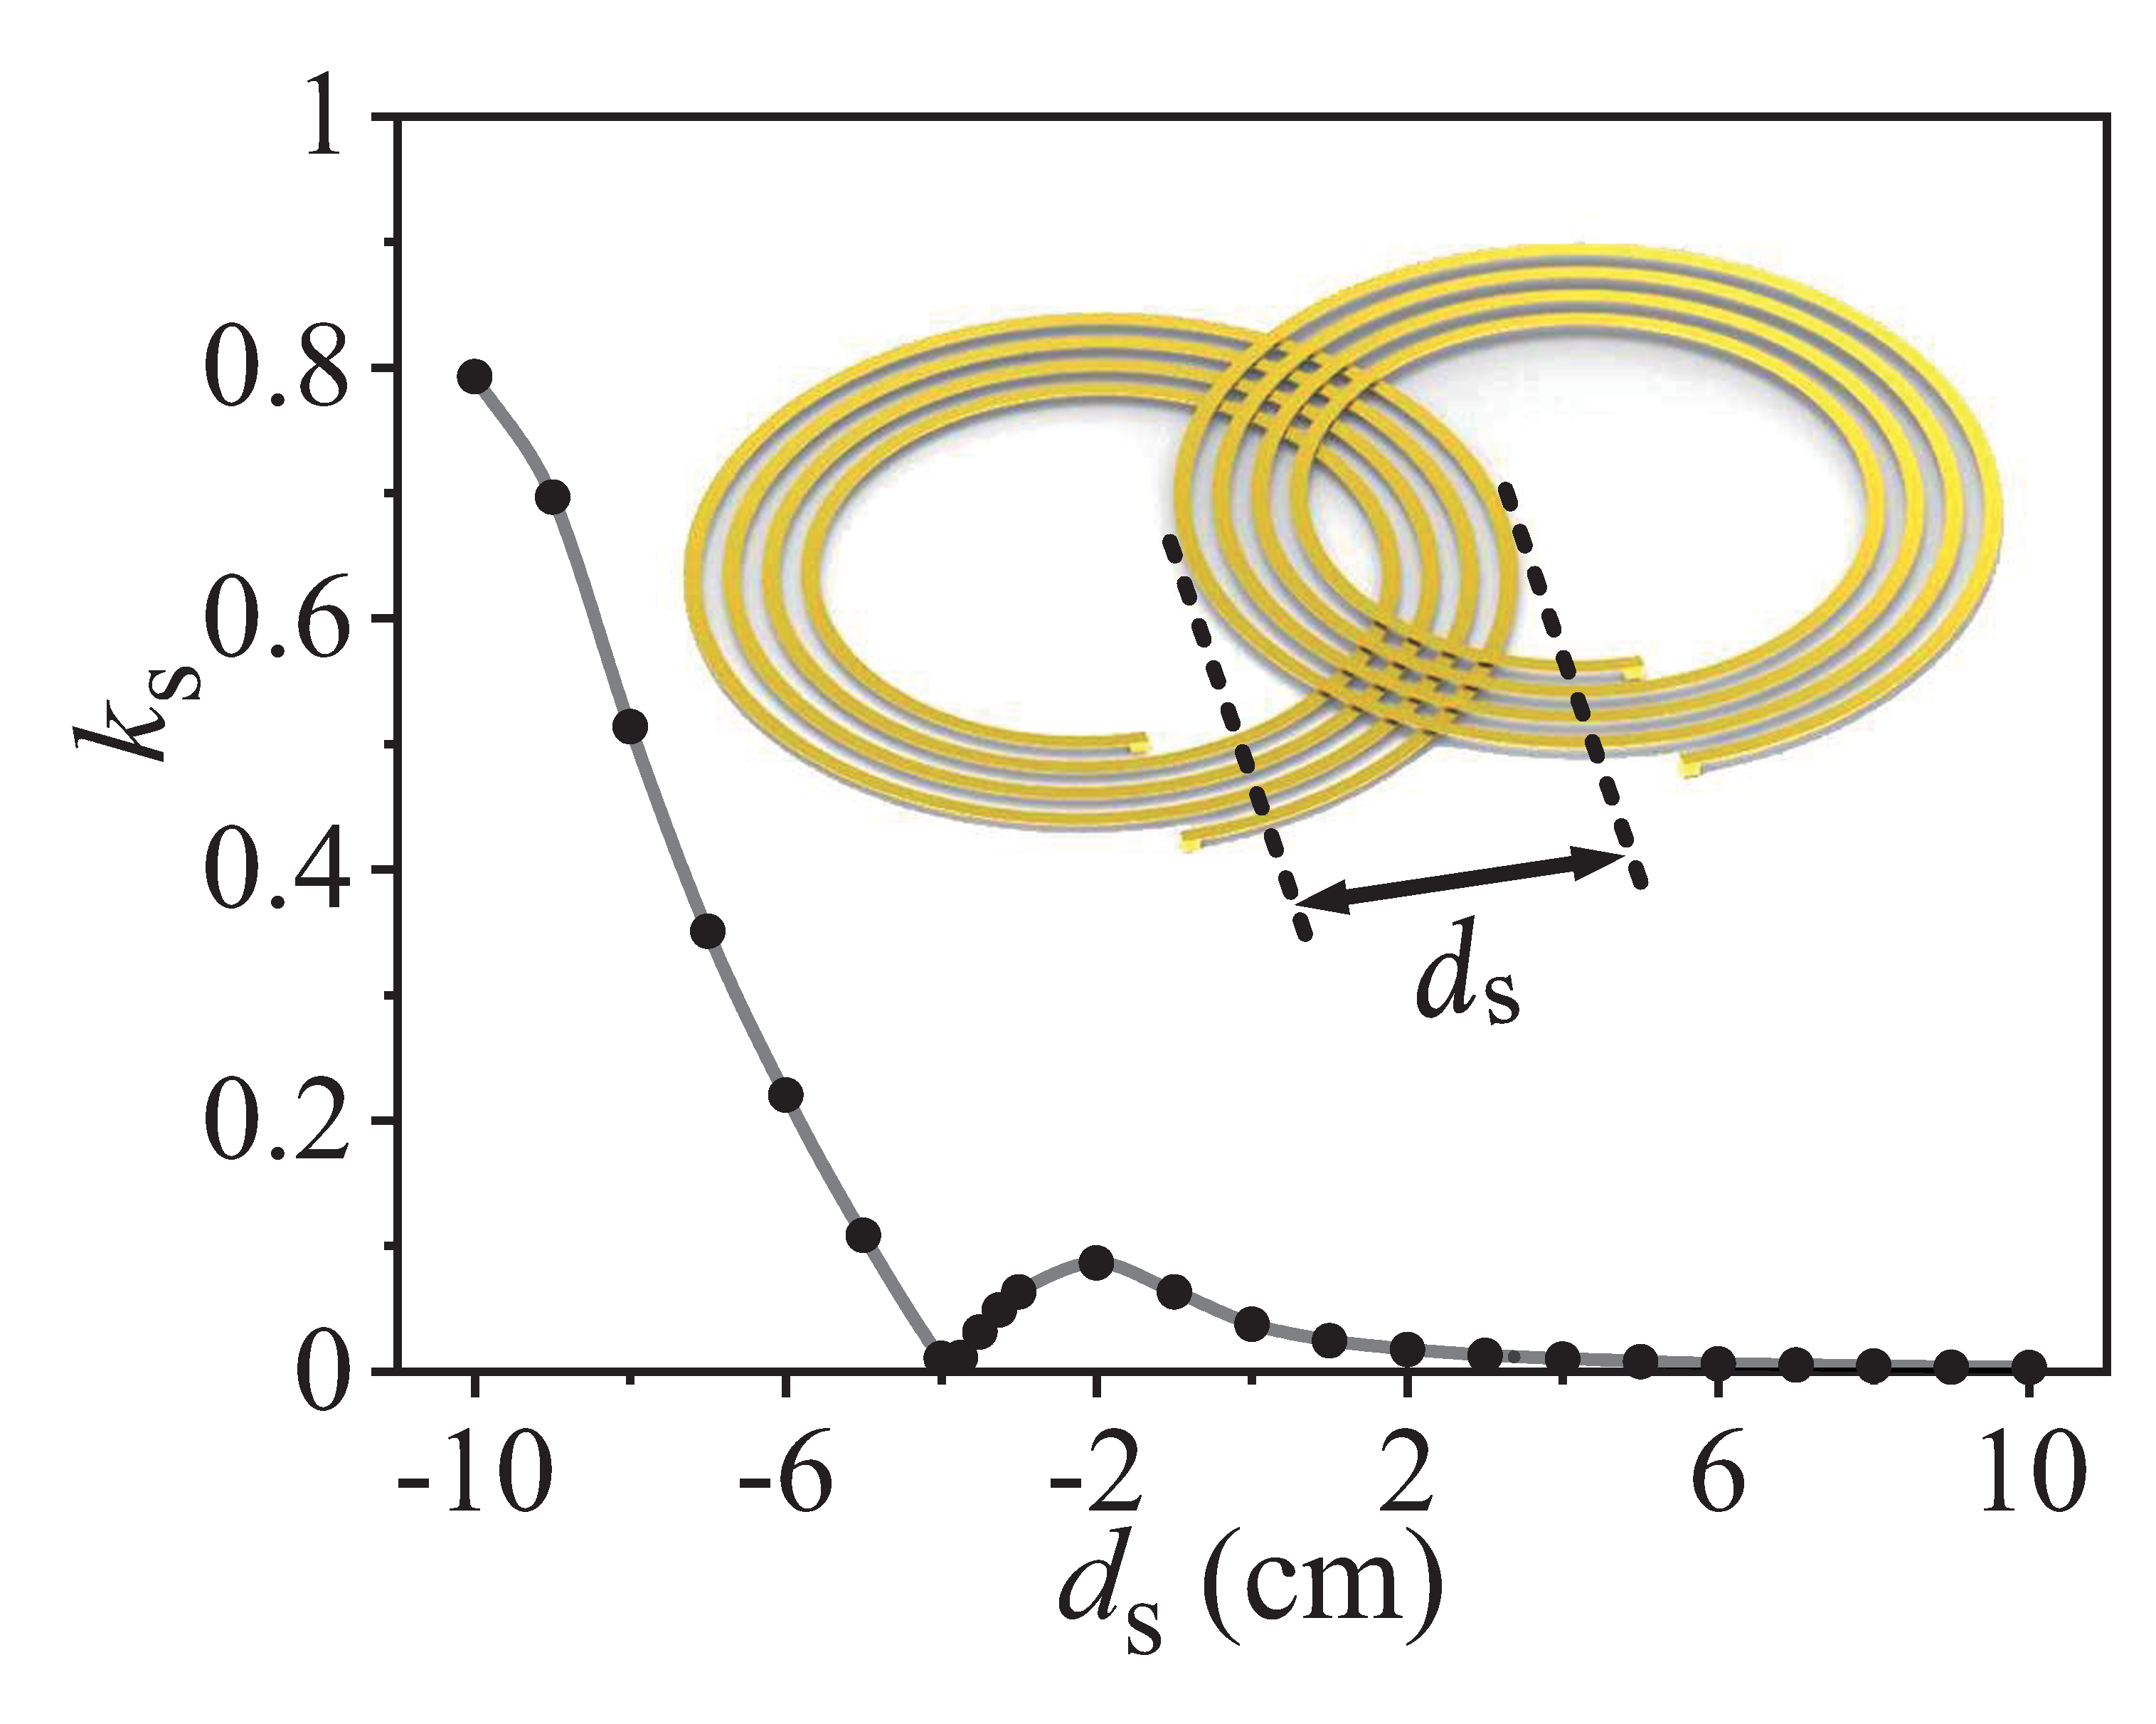
\includegraphics[width=4.22cm]{fig/fig8a.eps}}
    \subfigure[]{
    \label{fig:s10}
    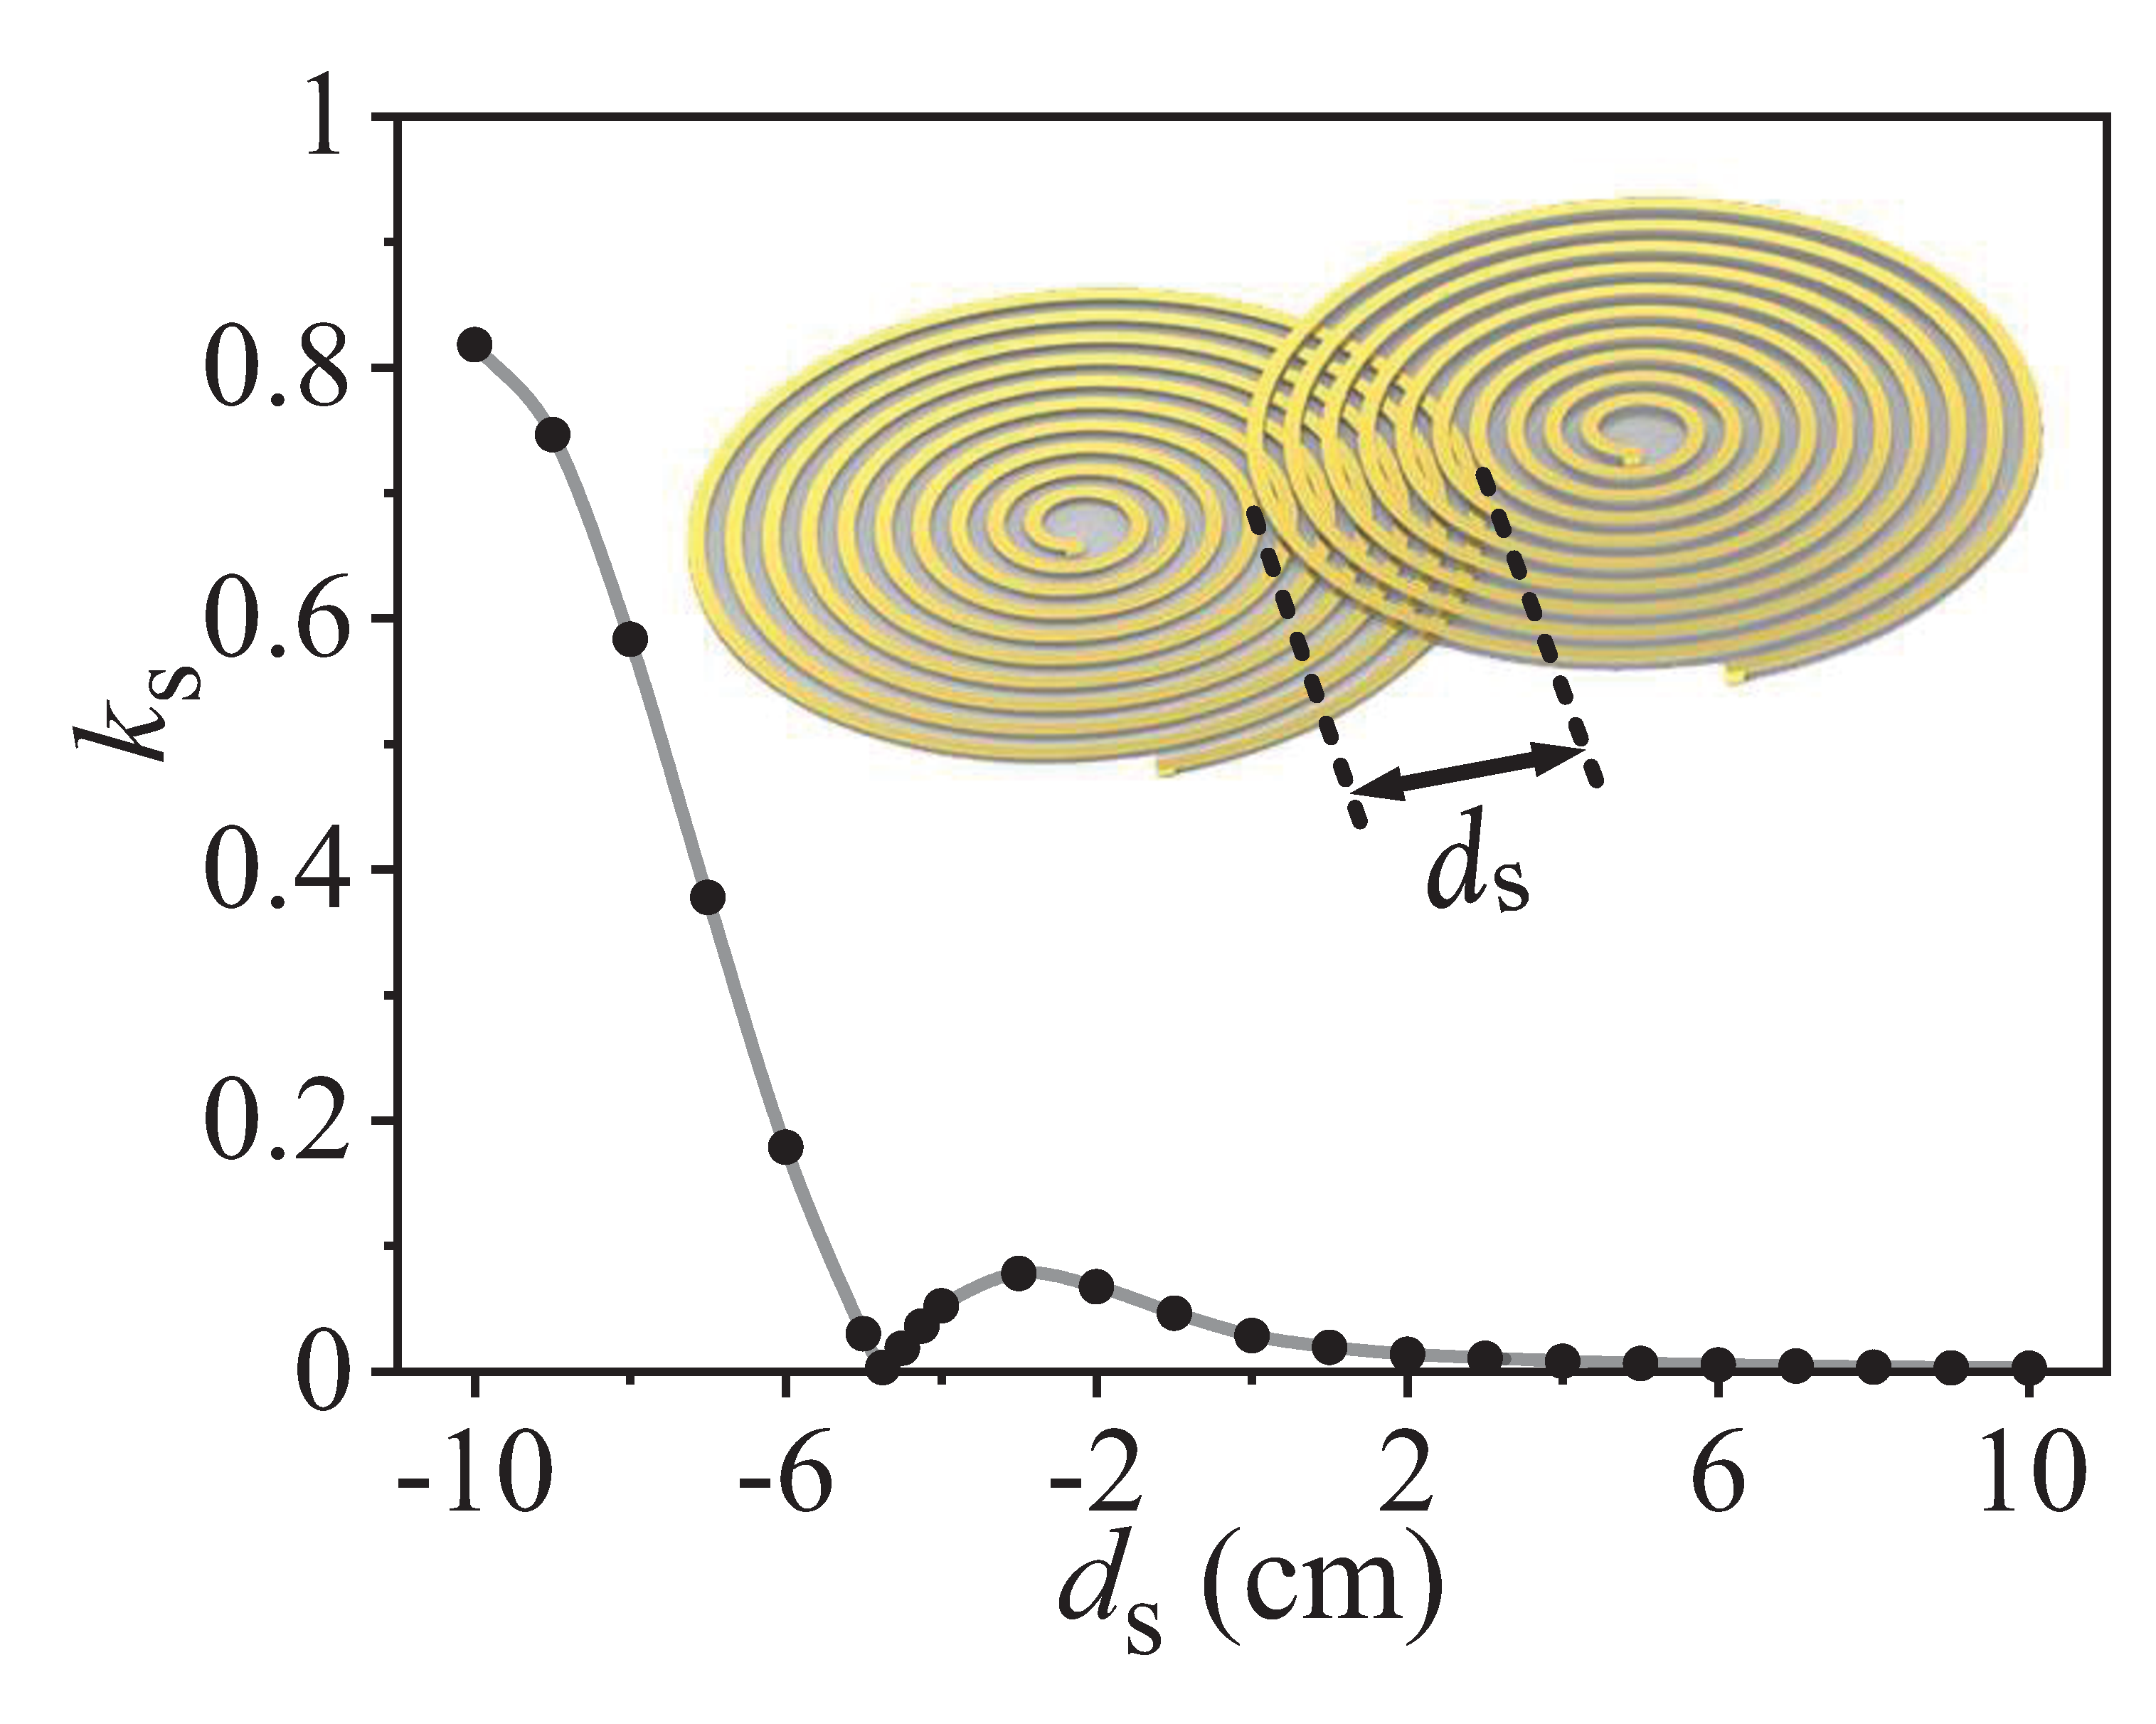
\includegraphics[width=4.22cm]{fig/fig8b.eps}}\
    \caption{Cross coupling coefficient versus $d_{\rm s}$ in spiral coils~(10~cm diameter). (a) 4 turns. (b) 10 turns (a coil pattern exists in the center).}
    \label{fig:scoils}
\end{figure}

\begin{figure*}[ht!]
    \centering
    \subfigure[]{
    \label{xdegree}
    \includegraphics[width=5.5cm]{fig/fig9a.eps}}
    \subfigure[]{
    \label{x1}
    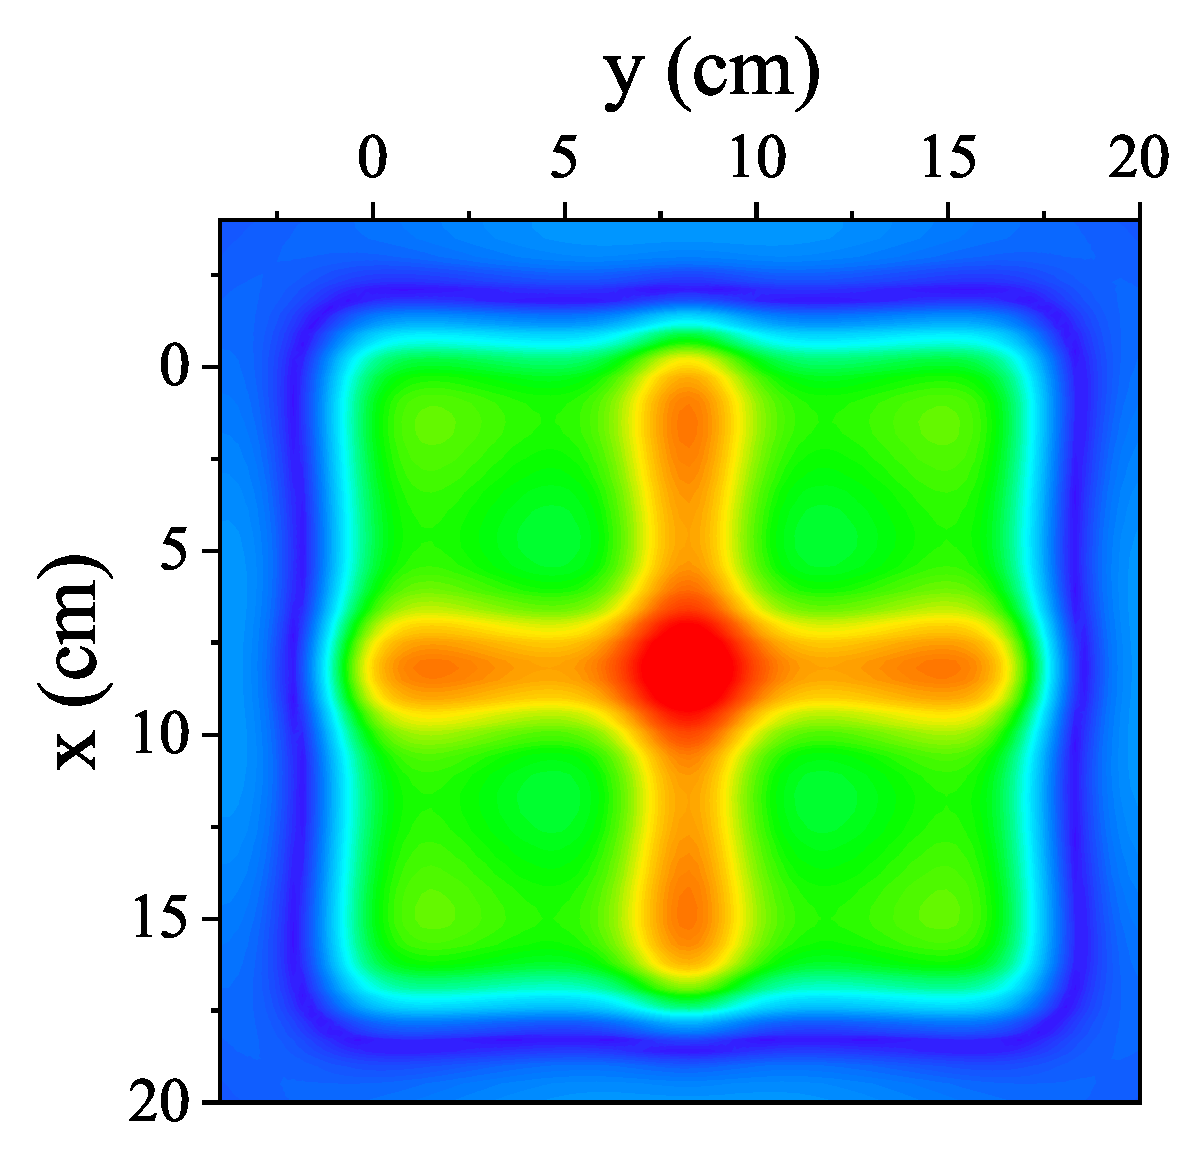
\includegraphics[height=4cm]{fig/fig9b.eps}}
    \subfigure[]{
    \label{x2}
    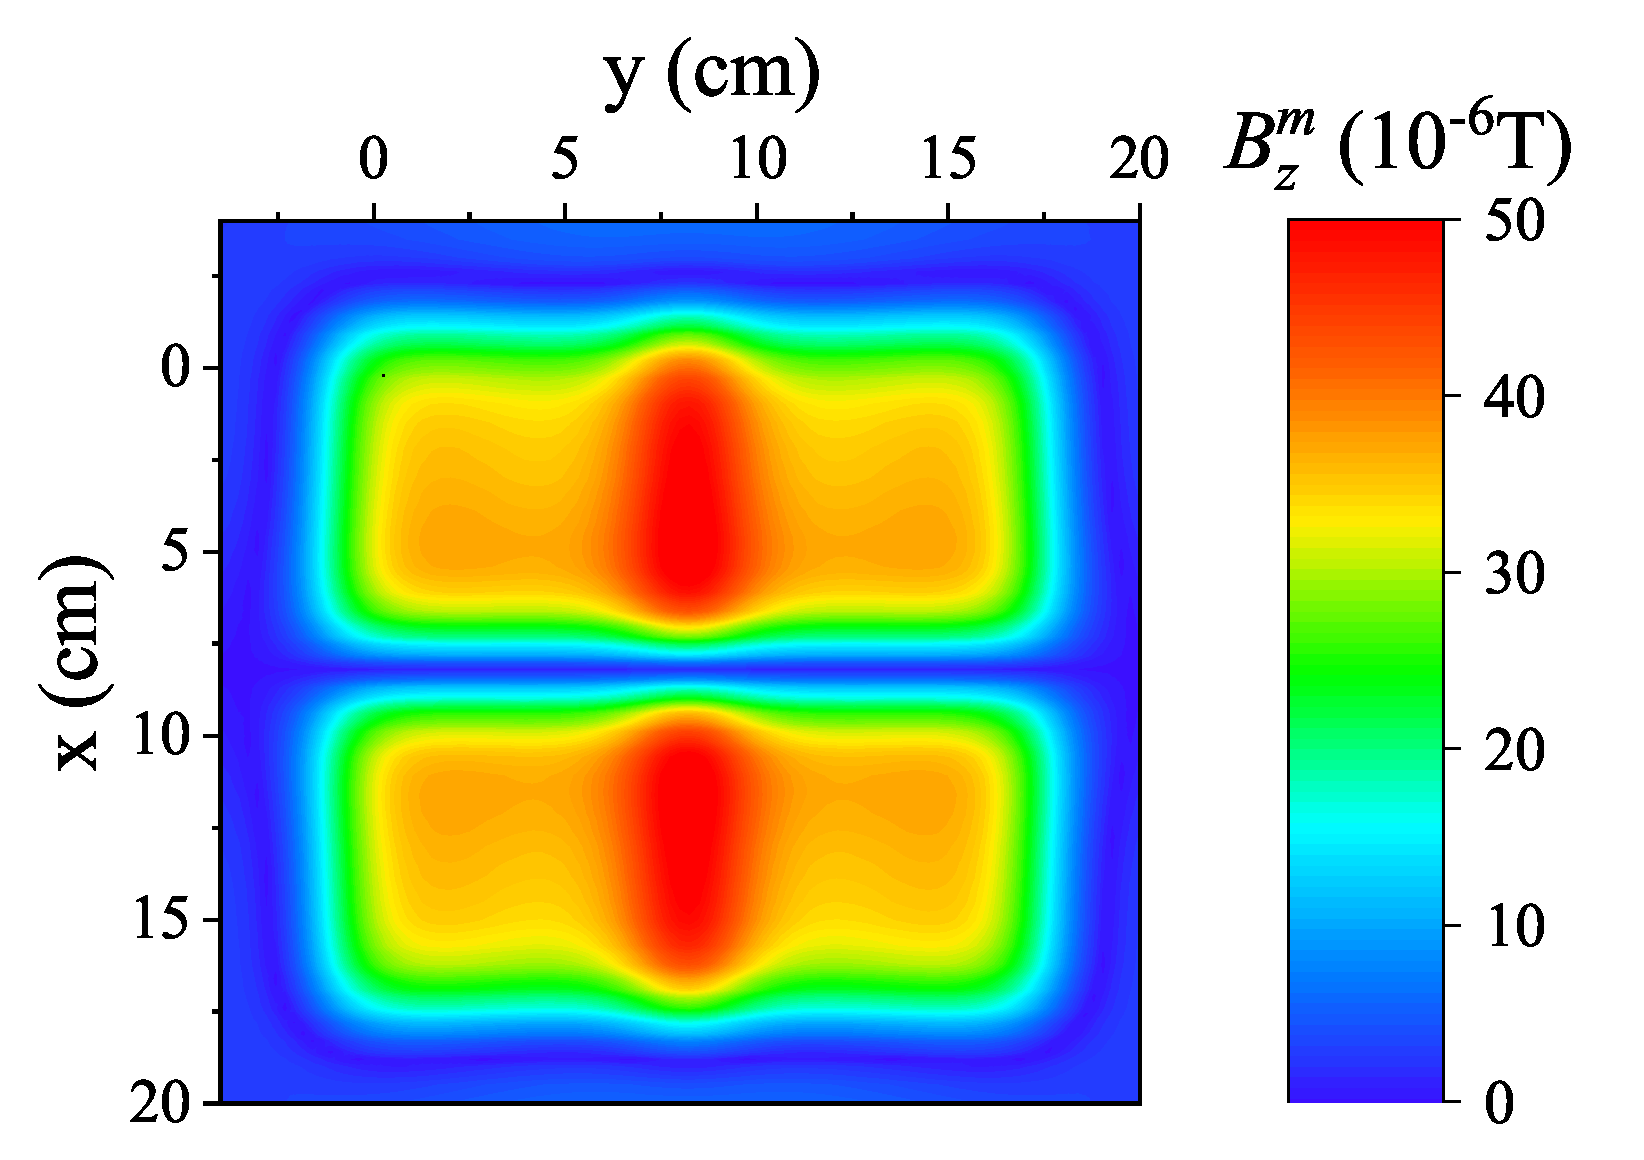
\includegraphics[height=4cm]{fig/fig9c.eps}}
    %\hspace{3cm}
    \subfigure[]{
    \centering
    \label{y1}
    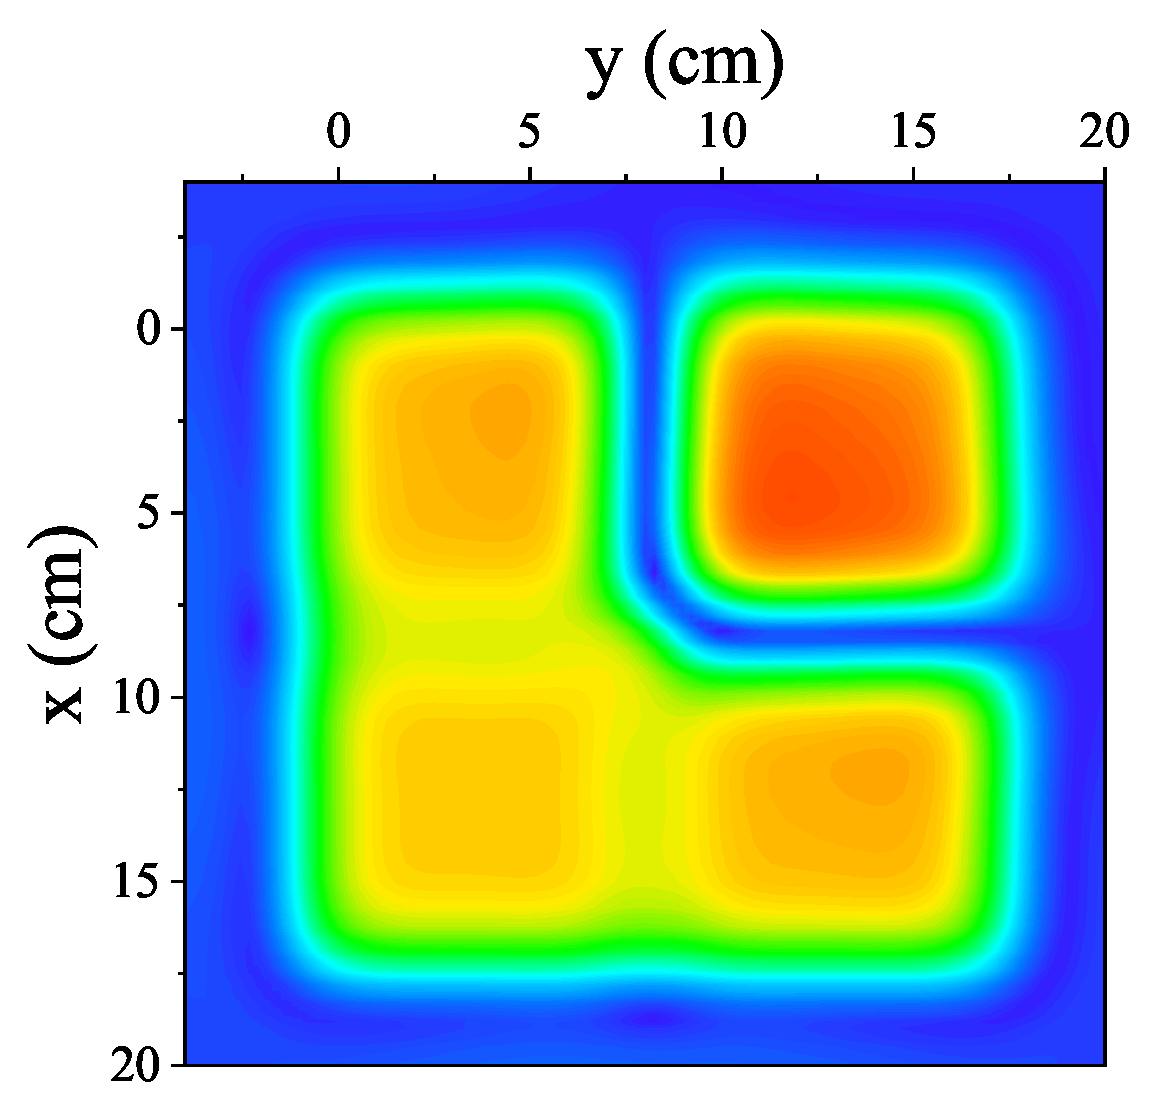
\includegraphics[height=3.85cm]{fig/fig9d.eps}}
    \hspace{1.3cm}
    \subfigure[]{
    \label{r1}
    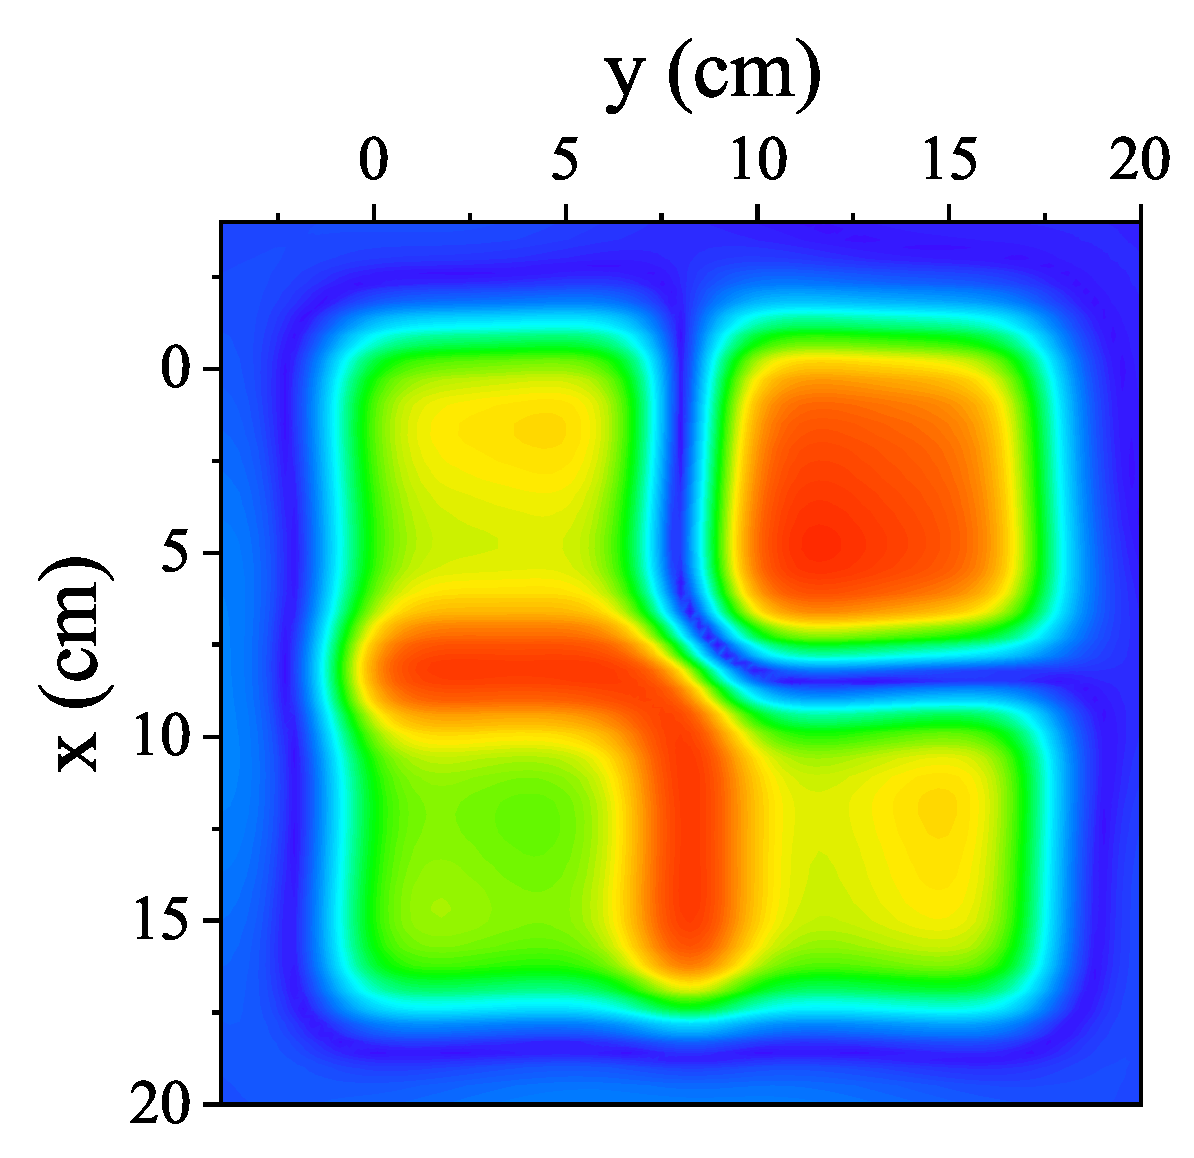
\includegraphics[height=4.05cm]{fig/fig9e.eps}}
    \hspace{-0.1cm}
    \subfigure[]{
    \label{r2}
    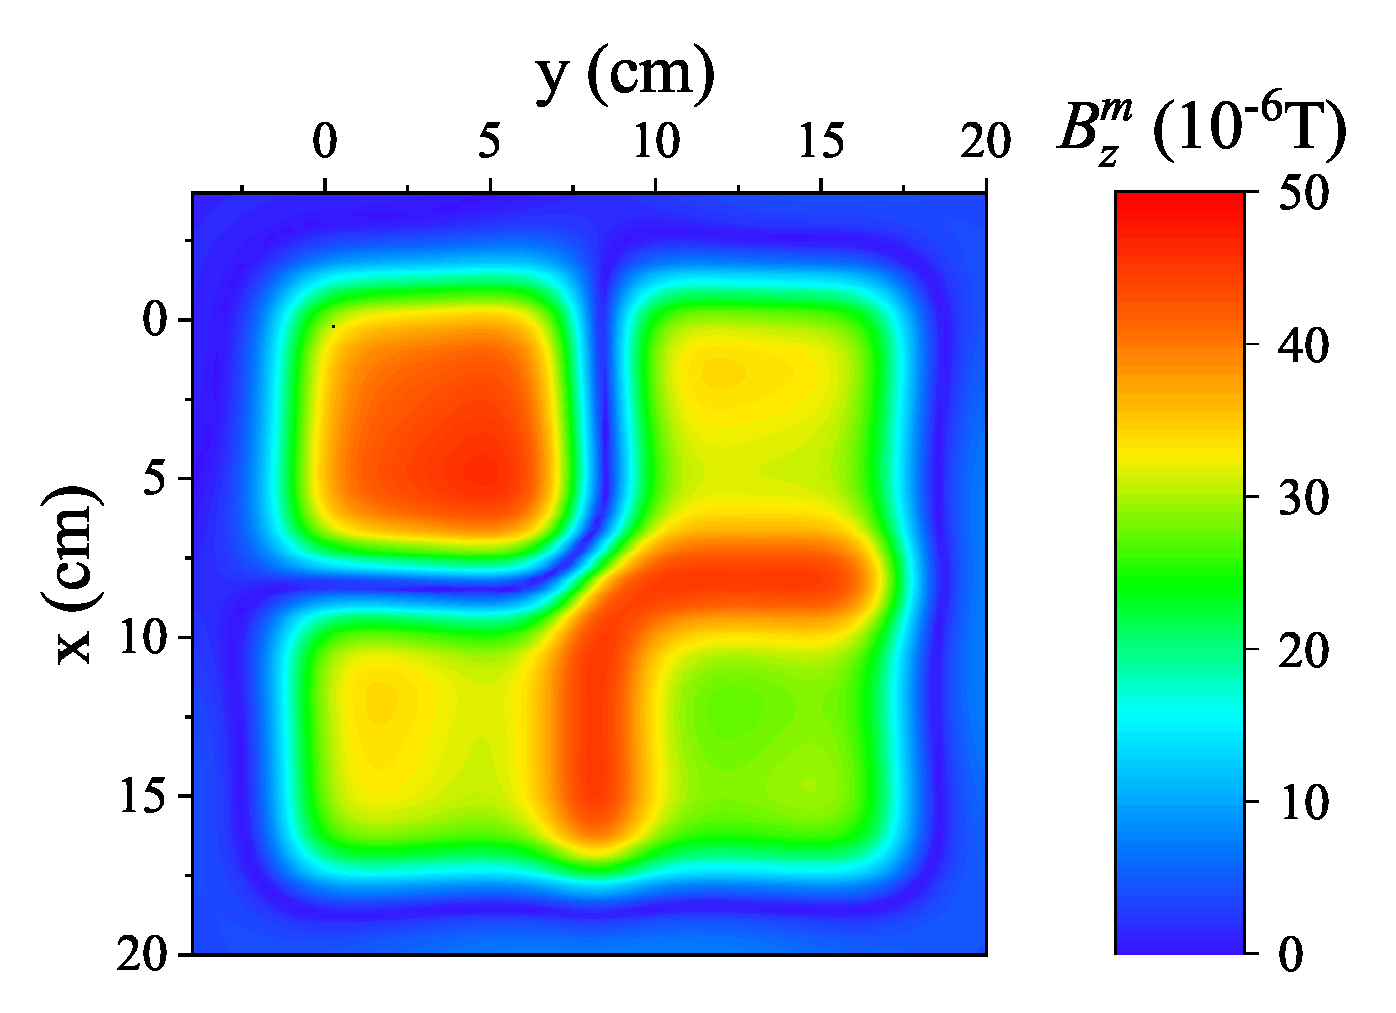
\includegraphics[height=4.05cm]{fig/fig9f.eps}}\
    %\rule{17cm}{0.8pt}
    \caption{Calculation results of B-field ADFs generated by a 2$\times$2 planar Tx-coil array~($z$=2.5~cm). (a) Layout and coordinates. (b) $\theta_1 = 0 {}^{\circ}$, $\theta_2 = 0 {}^{\circ}$, $\theta_3 = 0 {}^{\circ}$ and $\theta_4 = 0 {}^{\circ}$. (c) $\theta_1 = 0 {}^{\circ}$, $\theta_2 = 0 {}^{\circ}$, $\theta_3 = -180 {}^{\circ}$ and $\theta_4 = -180 {}^{\circ}$. (d) $\theta_1 = -180 {}^{\circ}$, $\theta_2 = 0 {}^{\circ}$, $\theta_3 = -180 {}^{\circ}$ and $\theta_4 = -90 {}^{\circ}$. (e) $\theta_1 = -180 {}^{\circ}$, $\theta_2 = 0 {}^{\circ}$, $\theta_3 = -180 {}^{\circ}$ and $\theta_4 = -180 {}^{\circ}$. (f) $\theta_1 = 180 {}^{\circ}$, $\theta_2 = 0 {}^{\circ}$, $\theta_3 = 0 {}^{\circ}$ and $\theta_4 = 0 {}^{\circ}$.}
    \label{3deg1}
\end{figure*}
\begin{figure*}[ht!]
    \centering
    \vspace{-0.3cm}
    \subfigure[]{
    \label{bdegree}
    \includegraphics[height=4cm]{fig/fig10a.eps}}
    \subfigure[]{
    \label{b1}
    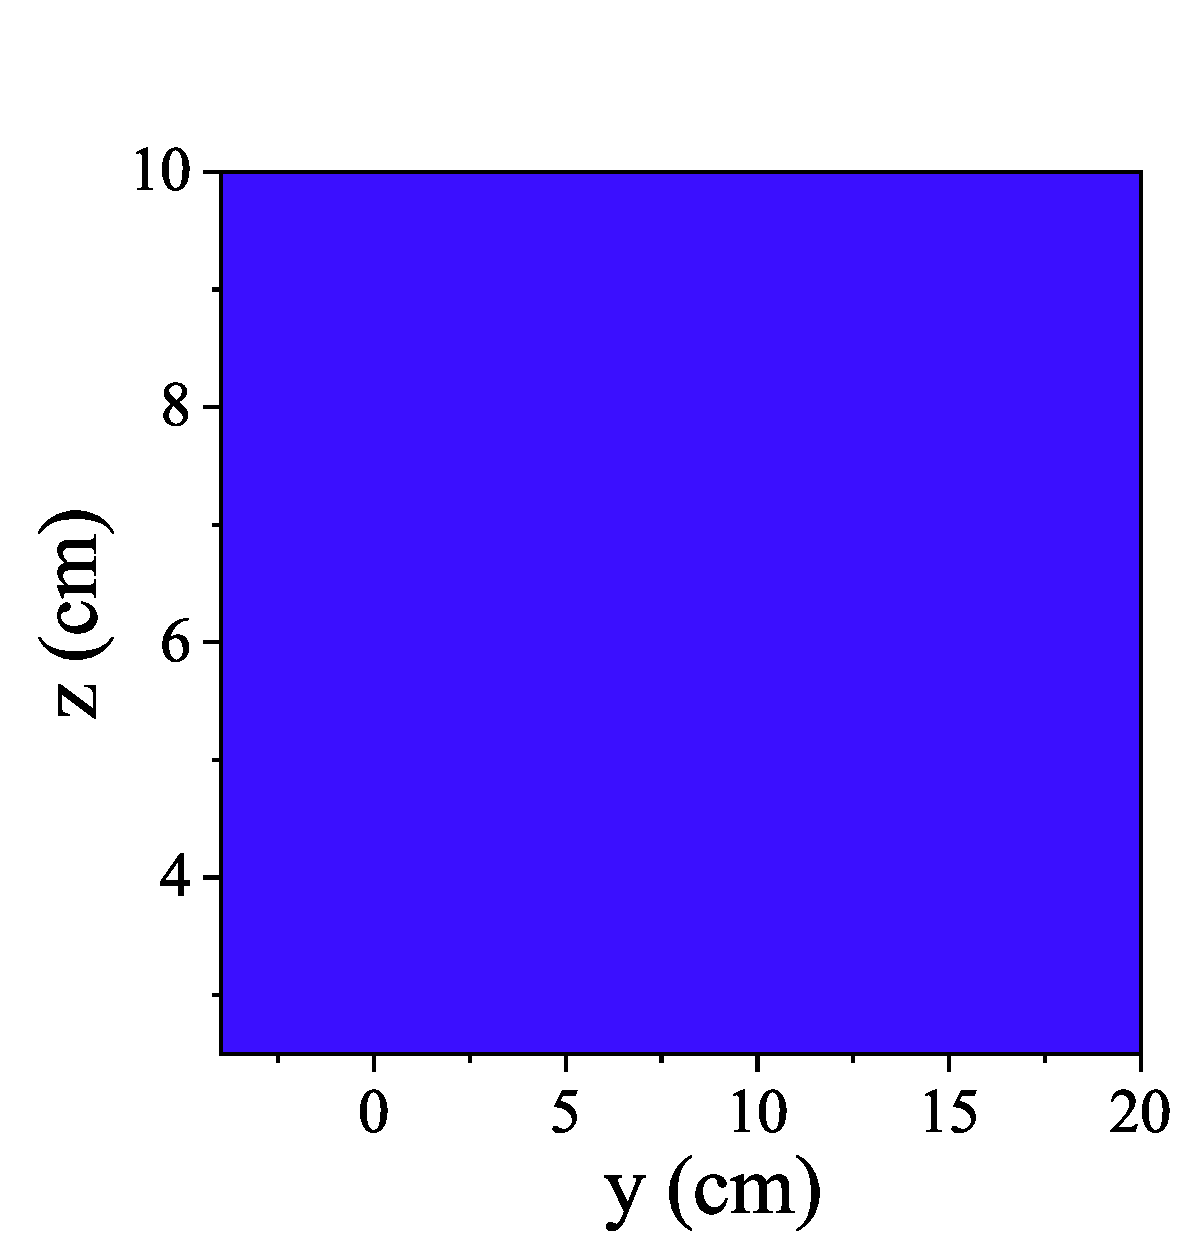
\includegraphics[height=4.3cm]{fig/fig10b.eps}}
    \subfigure[]{
    \label{b2}
    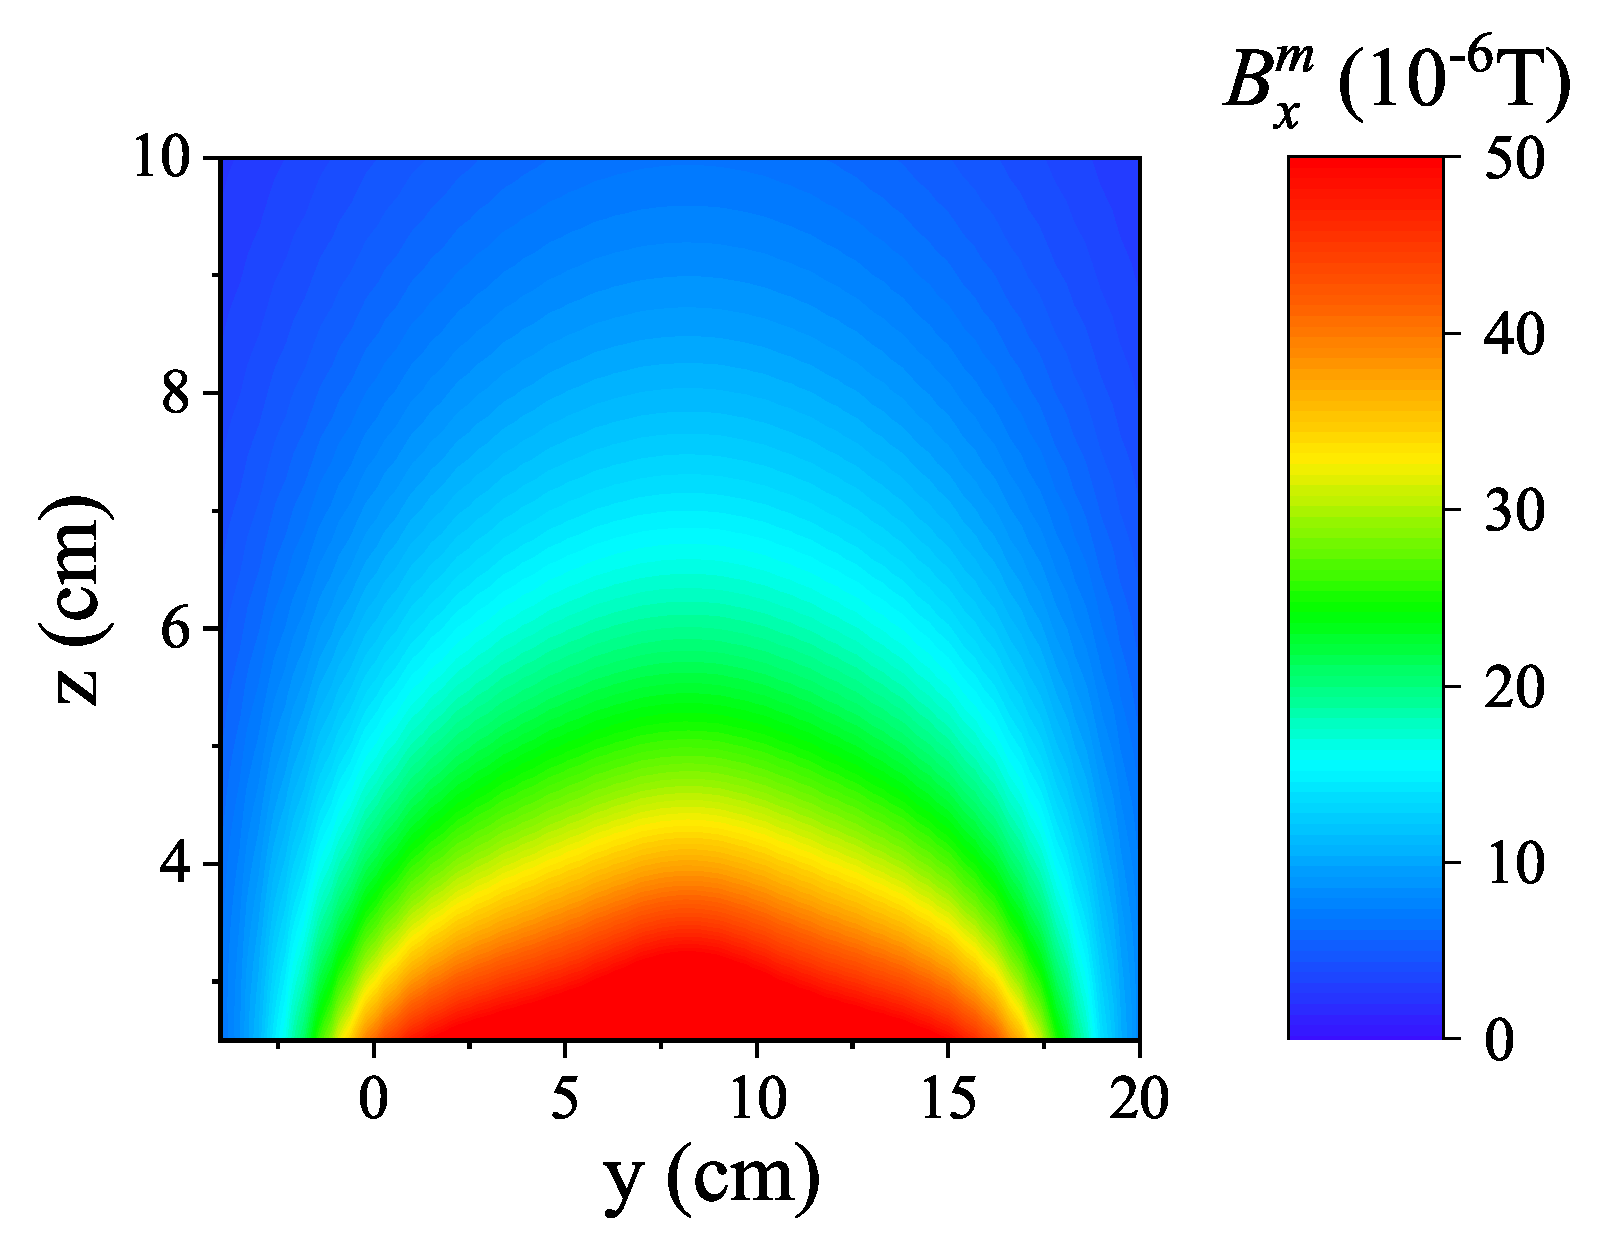
\includegraphics[height=4.27cm]{fig/fig10c.eps}}
    \subfigure[]{
    \label{zdegree}
    \includegraphics[height=4cm]{fig/fig10d.eps}}
    \hspace{0.1cm}
    \subfigure[]{
    \label{z1}
    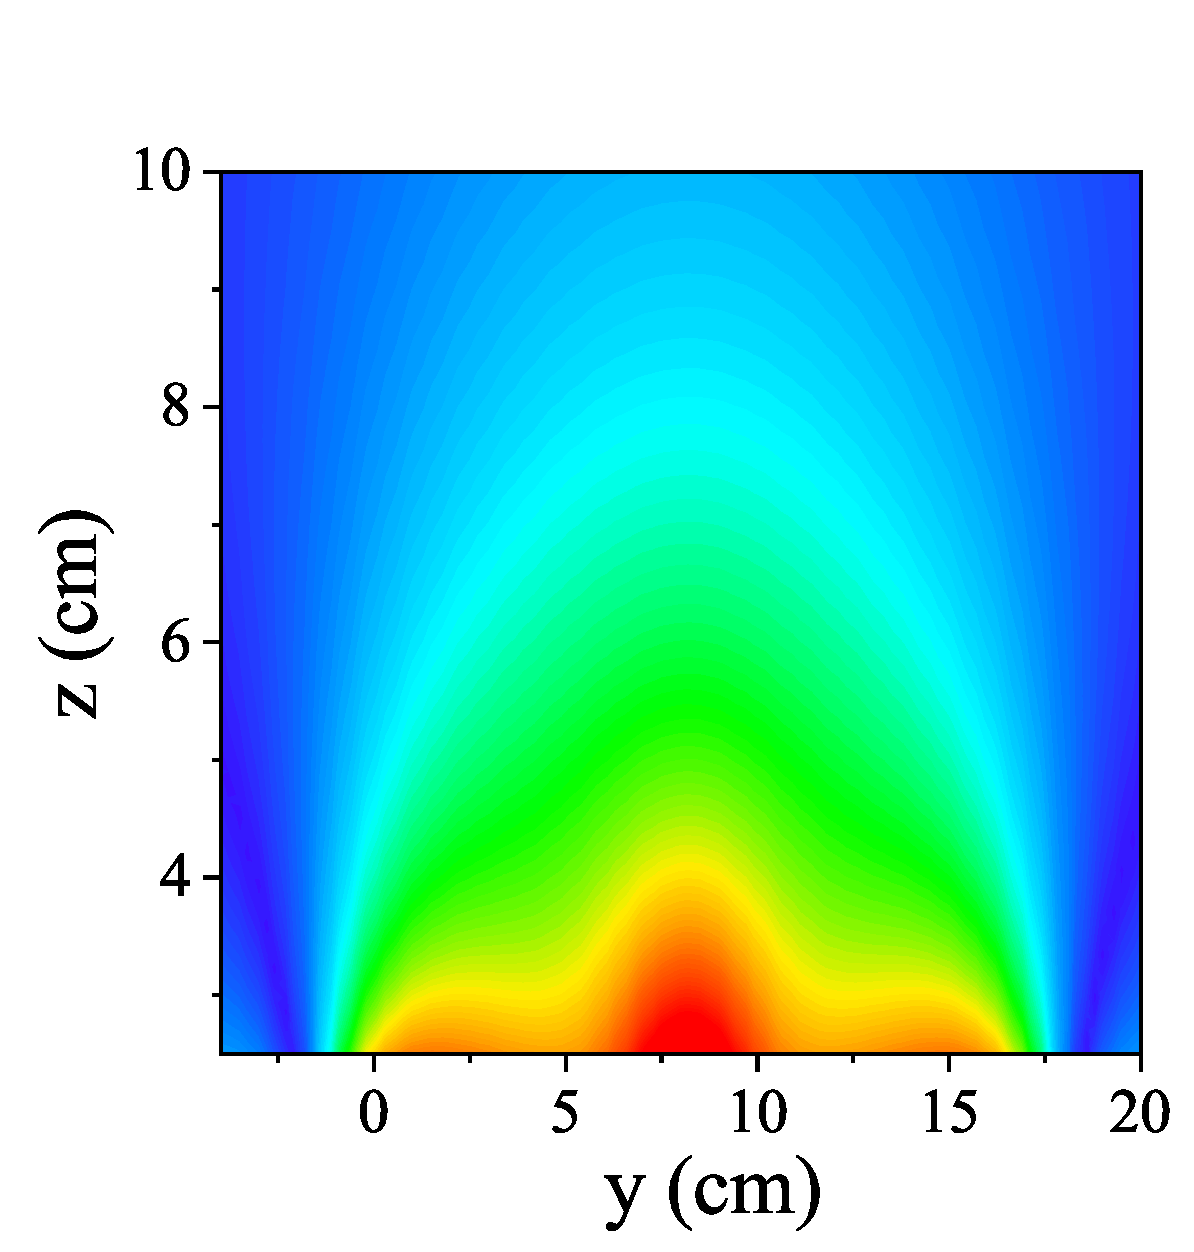
\includegraphics[height=4.3cm]{fig/fig10e.eps}}
    \subfigure[]{
    \label{z2}
    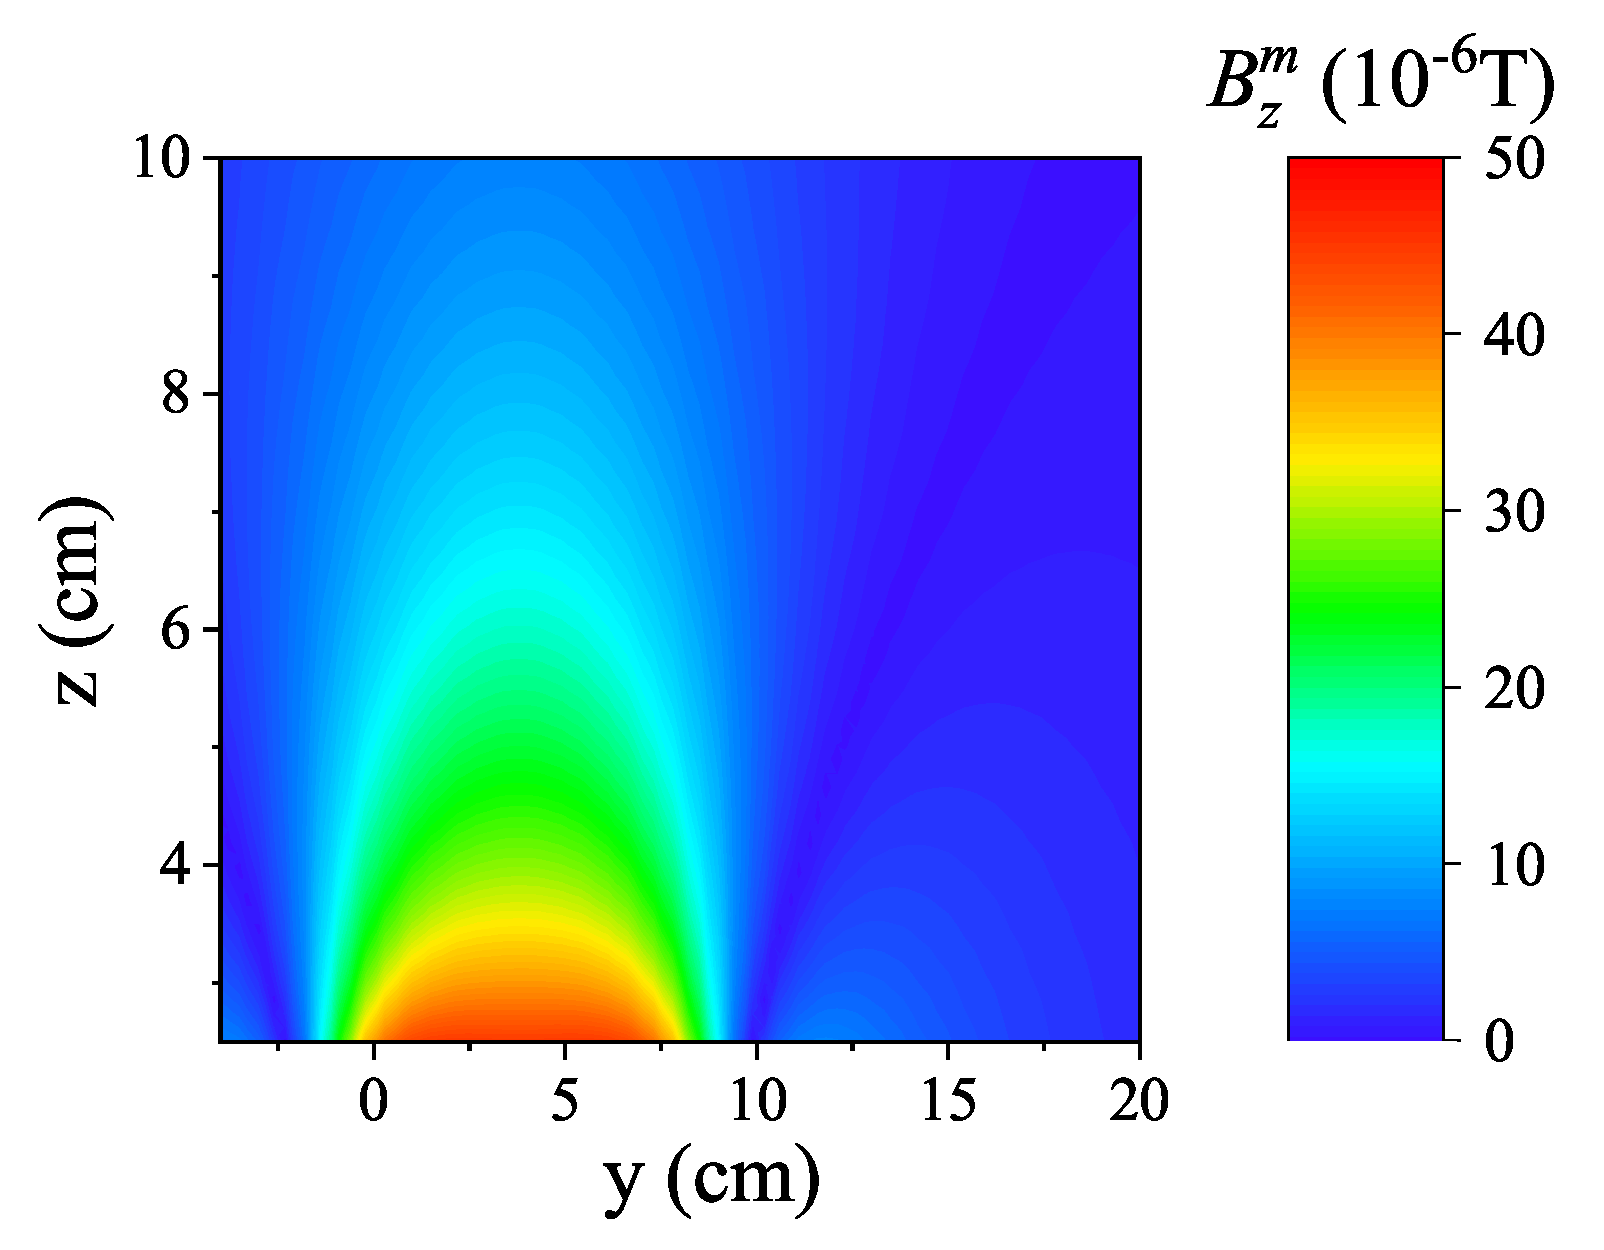
\includegraphics[height=4.27cm]{fig/fig10f.eps}}
    \caption{Calculation results of B-field ADFs generated by a 2$\times$2 planar Tx-coil array~($x$=8.2~cm). (a) Layout and coordinates for Fig.~\ref{b1} and Fig.~\ref{b2}. (b) $\theta_1 = 0 {}^{\circ}$, $\theta_2 = 0 {}^{\circ}$, $\theta_3 = 0 {}^{\circ}$, and $\theta_4 = 0 {}^{\circ}$. (c) $\theta_1 = 0 {}^{\circ}$, $\theta_2 = 0 {}^{\circ}$, $\theta_3 = 180 {}^{\circ}$, and $\theta_4 = 180 {}^{\circ}$. (d) Layout and coordinates for Fig.~\ref{z1} and Fig.~\ref{z2}. (e) $\theta_1 = 0 {}^{\circ}$, $\theta_2 = 0 {}^{\circ}$, $\theta_3 = 0 {}^{\circ}$, and $\theta_4 = 0 {}^{\circ}$. (f) $\theta_1 = 0 {}^{\circ}$, $\theta_2 = 0 {}^{\circ}$, $\theta_3 = 180 {}^{\circ}$, and $\theta_4 = 0 {}^{\circ}$.}
    \label{3deg2}
\end{figure*}

\section{Magnetic Field Shaping Effects}
\label{sec:shaping}

Fig.~\ref{3deg1} and Fig.~\ref{3deg2} show magnetic field shaping effects in $xy$ plane and $yz$ plane, taking a 2$\times$2 Tx-coil array as an example. Compared with 3D figures, these 2D figures with B-field amplitude distribution more clearly demonstrate the shaping effects. Here the operating frequency is 6.78~MHz. The currents in the Tx coils have the same amplitude but different phases (i.e., phase shift modulation). The side length of all coils $l$ is 10~cm, and the coil distance $d$ is -1.24~cm to minimize the cross coupling. As a preliminary study, the magnetic field shaping effects are individually verified with phases of 0, 90, 180, 270 degrees in the Tx coils. The combinations of phases in Figs~\ref{3deg1} and \ref{3deg2} are especially selected to show an obvious magnetic field shaping effect.

As shown in Fig.~\ref{x1}, if there is no phase difference in the Tx-coil currents, the $z$-direction B-field amplitude distribution on the $xy$ plane (i.e., $B_z^m$) has its peak at the center of the observation plane ($z$=2.5~cm). If the phase shift is applied, such as in Fig.~\ref{x2}, the peak in the $xy$ plane will be split into two peaks along the $x$ axis and be actually further strengthened. Note that the peak can also appear above the non-overlap areas, such as shown in Fig.~\ref{y1}. These figures, namely Fig.~\ref{x1}--Fig.~\ref{y1}, demonstrate the possibility of controlling the $z$-direction magnetic field distribution over the $xy$ plane by changing the phases of the Tx-coil currents. This new capability can be utilized to enhance the adaptability of the power transfer to the horizontal misalignment (i.e., over the $xy$ plane) of an Rx coil, as experimentally verified in the following Section~\ref{sec:exp}. Fig.~\ref{r1} and Fig.~\ref{r2} further show that the two peaks of the B-field distribution can actually rotate over the $xy$ plane through the coil current phase shift modulation, which proves an additional degree of freedom in the magnetic field shaping.

Similarly, Fig.~\ref{b1} and Fig.~\ref{b2} show the magnetic field shaping effect in $x$ direction over $yz$ plane, namely $B_x^m$~($x$=8.2~cm). Both the B-field strength and distribution can be adjusted through the Tx current phase shift modulation. As shown in Fig.~\ref{b2}, unlike the conventional signal Tx-coil transmitter, the planar Tx-coil array is able to transfer power to an Rx coil that is perpendicular to the plane of the transmitter. Similar results can be seen in Fig.~\ref{z1} and Fig.~\ref{z2}, which show the effect in $z$ direction, namely $B_z^m$~($x$=8.2~cm). All the above calculation results indicate a promising aspect of the planar (i.e., 2D) Tx-coil array-based magnetic field shaping, namely the controllable magnetic field distribution in 3D space. This advantage will significantly improve the adaptability of WPT to receivers with 3D positions and orientations in actual environments. \\

\begin{figure*}[ht!]
    \centering
    \subfigure[]{
    \label{circuits}
    \includegraphics[height=5.5cm]{fig/fig11a.eps}}
    \subfigure[]{
    \label{4types}
    \includegraphics[height=5.5cm]{fig/fig11b.eps}}\
    \caption{A 6.78~MHz WPT system with an extendable planar Tx-coil array. (a) Circuit model. (b) Tx coils (\#1--3) and Rx coil.}
    \label{circoil}
\end{figure*}

\section{Experimental Implementation}
\label{sec:exp}

\subsection{Configuration and Setup}
\begin{figure}[b!]
    \centering
    \vspace{-0.3cm}
    \centerline{\includegraphics[width=9.5cm]{fig/fig12.eps}}
    \caption{Final experimental 6.78-MHz WPT system employing the proposed extendable planar Tx-coil array.}
    \label{system}
\end{figure}
Fig.~\ref{circuits} shows the circuit model of an example WPT system with an extendable planar Tx-coil array and a receiver. The transmitter includes multiple Class E PAs operating at 6.78 MHz to separately drive their corresponding Tx coils. And the receiving side consists of an Rx coil and a Class E full-wave rectifier. The phase shift between the drive signals of the PAs is modulated to generate Tx-coil currents with different phases. In the present experimental system, there are four PAs and four Tx coils.

Fig.~\ref{4types} shows three types of Tx coils for comparison purposes.
\begin{enumerate}
  \item Tx\#1: Single large Tx coil;
  \item Tx\#2: 2$\times$2 Tx-coil array without overlap;
  \item Tx\#3: 2$\times$2 Tx-coil array with overlap to minimize the average cross coupling $k_{\rm avg}$.
\end{enumerate}

The final experimental 6.78~MHz WPT system in Fig.~\ref{system} employs the same configuration in Fig.~\ref{circoil}. The PA switches $Q_{1-4}$ use GaN transistors (GS61004B). A 10$\Omega$ dc load is emulated using an electronic load. Two waveform generators are utilized to generate four-channel phase shifted PA driving signals. In actual scenarios, both FPGA and dedicated phase delay ICs can be applied to implement the phase shift modulation~\mbox{\cite{song2020universal,liu2020dual}}. Note that in Fig.~\mbox{\ref{system}}, the Rx coil is perpendicular to the Tx-coil array. All the parameters of the three types of Tx PCB coils are listed in Table~\ref{coils}. The quality factor of Tx\#1 is much lower because the coil parasitic resistance grows faster than inductance when the coil size increases. In Tx\#3, the distance $d$ between adjacent Tx coils is determined to minimize the coil cross coupling~[refer to Section~\ref{sub:minimize}]. For the sake of simplicity, the Rx coil is as same as a single Tx coil in Tx\#2 and Tx\#3.
\renewcommand\arraystretch{1.1}
\begin{table}[ht!]
%\vspace{-3mm}
\caption{Major Parameters of Three Types of Tx Coils (6.78~MHz). }
\vspace{-6mm}
%\renewcommand{\arraystretch}{1}
\begin{center}
\resizebox{\columnwidth}{!}{
\begin{tabular}{l c c c}
\toprule[1pt] \\[-3mm]
Parameters               & Tx\#1  & Tx\#2  & Tx\#3   \\%[0.9ex]
\midrule[0.5pt] \\[-3mm]
Inductance ($ \mu $H)    & 10.76    & 3.32       & 3.32         \\

Parasitic resistance ($ \Omega $)    & 3.96       & 0.61       & 0.61       \\

Quality factor   & 115.8       & 231.9       & 231.9       \\

Coil array area (cm$^2$)  & 20.0$\times$20.0  & 20.0$\times$20.0   & 17.8$\times$17.8  \\

Coil distance $d$ (cm)    & n/a   & 1       & -1.24  \\

Number of coils    & 1       & 4       & 4  \\

Number of turns    & 4       & 4       & 4  \\

Coil trace width (cm) & 0.2  & 0.2     & 0.2  \\

Coils trace spacing (cm) & 0.1  & 0.1   & 0.1  \\

Coils trace thickness (cm)  & 0.007     & 0.007   & 0.007  \\
[0.3ex]
\bottomrule[1pt]
\end{tabular}
}
\label{coils}
\end{center}
\vspace{-2mm}
\end{table}

Table~\ref{coupling} lists the measured cross coupling coefficients in the two Tx-coil arrays (Tx\#2,3). Consistent with the above analysis via Fig.~\ref{k}, the type 1 cross coupling ($k_1$) is dominant and can be dramatically reduced by the optimized Tx-coil overlap design ($d$=-1.24~cm). This leads to a largely minimized average cross coupling coefficient $k_{\rm avg}$ (68.1\% reduction). It is known that a reflected impedance seen by an individual Tx coil is proportional to the square of the cross coupling coefficient~\cite{liu2020high}. For Tx\#3 array, the mutual interference among the coils is much smaller than that in Tx\#2 array, which helps improve the loading condition of the current-mode Class E PAs. Note that in the present overlap design, $k_2$'s are actually increased to reduce the more dominant $k_1$'s. 

\renewcommand\arraystretch{1.1}
\begin{table}[ht!]\small
%\vspace{-3mm}
\caption{Measurement Results of Tx-Coil Cross Coupling. }
%\renewcommand{\arraystretch}{1}
\vspace{-3mm}
\begin{center}
\begin{tabular}{l c c c}
\toprule[1pt] %\\[-1mm]
Tx-coil pair / $k_{\rm avg}$   & Cross coupling type & Tx\#2  & Tx\#3  \\%[0.9ex]
\midrule[0.5pt] %\\[-2mm]
No.~1 -- No.~2    & Type 1 & 0.094       & 0.010  \\

No.~1 -- No~.3    & Type 2 & 0.020       & 0.048  \\

No.~1 -- No.~4    & Type 1 & 0.092       & 0.006  \\

No.~2 -- No.~3    & Type 1 & 0.092       & 0.013  \\

No.~2 -- No.~4    & Type 2 & 0.020       & 0.044  \\

No.~3 -- No.~4    & Type 1 & 0.094       & 0.009  \\

$k_{\rm avg}$  & n/a & 0.069       & 0.022  \\
%[0.6ex]
\bottomrule[1pt]
\end{tabular}
%}
\label{coupling}
\end{center}
\vspace{-2mm}
\end{table}

\subsection{PA Parameter Selection}

Thanks to the matching network design (T$-$type here) developed in Ref.~\cite{liu2016novel}, the Class E PAs are possible to maintain an almost constant output current amplitude (i.e., current-mode) when there are variations in their load impedance, such as due to changes in the position and orientation of the Rx coil~[see Fig.~\ref{circuits}]. The target variation range of PA load impedance can be first determined by experimental testing. Then, as mentioned in Ref.~\mbox{\cite{liu2016novel}}, the classical Class E PA can be designed targeting an intermediate dc load~(22~$\Omega$ here), and the parameters of the T$-$type matching network are accordingly optimized to transform the varying load impedance to the PA high-efficiency region.

Table~\ref{tab:PA_para} lists the parameters of the PAs that drive Tx\#1--3. Note that the two inductors of the T$-$type matching network are absorbed by $L_0$ and $L_{\mathrm{tx}}$, respectively. The four PAs for Tx\#2 and Tx\#3 share the same set of parameters. Because of inevitable manufacturing errors, the combinations of $L_0$ and $C_0$ of the PAs are slightly different. In the Tx\#2 case, the strong cross coupling between the Tx coils (i.e., without the overlap design) further complicates the loading condition during the phase shift modulation, which makes the PA parameter design especially difficult~\cite{feng2020lccl}. As an example, Fig.~\ref{fig:impe} shows the trajectories of the PA load impedance $Z_{\mathrm{PA}}$ when $\theta _{1}$ and $\theta _{2}$ are 0, and $\theta _{3}$ and $\theta _{4}$ change from 0 to 360 degrees. Here $\eta_{\mathrm{PA}}$ is the efficiency of a single PA. The range of the PA load impedance variation is significantly suppressed with the overlap design (i.e., the case of Tx\#3). This certainly helps alleviate the difficulty in PA parameter selection. It again indicates the importance of the overlap design of the Tx-coil array.
\begin{table}[htbp]%\small
	\renewcommand\arraystretch{1.1}
  \centering
  \caption{PA Parameters for Tx\#1--3.}
  %\resizebox{\columnwidth}{!}{
    \begin{tabular}{c|cccccc}
    \toprule[1pt]
          & $L_\mathrm{1}$ & $C_\mathrm{s}$ & $C_\mathrm{0}$ & $L_\mathrm{0}$ & $C_\mathrm{1}$ & $C_\mathrm{tx}$ \\
          & ($ \mathrm{\mu} $H) & (pF) & (pF) & ($ \mathrm{\mu} $H) & (pF) & (pF) \\
          %\cline{2-7}
    \cmidrule[0.4pt](lr){1-1} \cmidrule[0.4pt](lr){2-7}
    Tx\#1 & 10    & 76    & \multicolumn{1}{c}{938} & \multicolumn{1}{c}{1.793} & 560   & 52 \\
    \cmidrule[0.4pt](lr){1-1} \cmidrule[0.4pt](lr){2-7}
    \makecell[c]{Tx\#2\\ \& \\Tx\#3} & 10    & 76    & \makecell[c]{760 (PA1)\\751 (PA2)\\750 (PA3)\\774 (PA4)} & \makecell[c]{1.930 (PA1)\\1.939 (PA2)\\1.940 (PA3)\\1.918 (PA4)} & 560   & 182 \\
    \bottomrule[1pt]
    \end{tabular}%
    %}
  \label{tab:PA_para}%
\end{table}%

\begin{figure}[h!]
    \centering
    \centerline{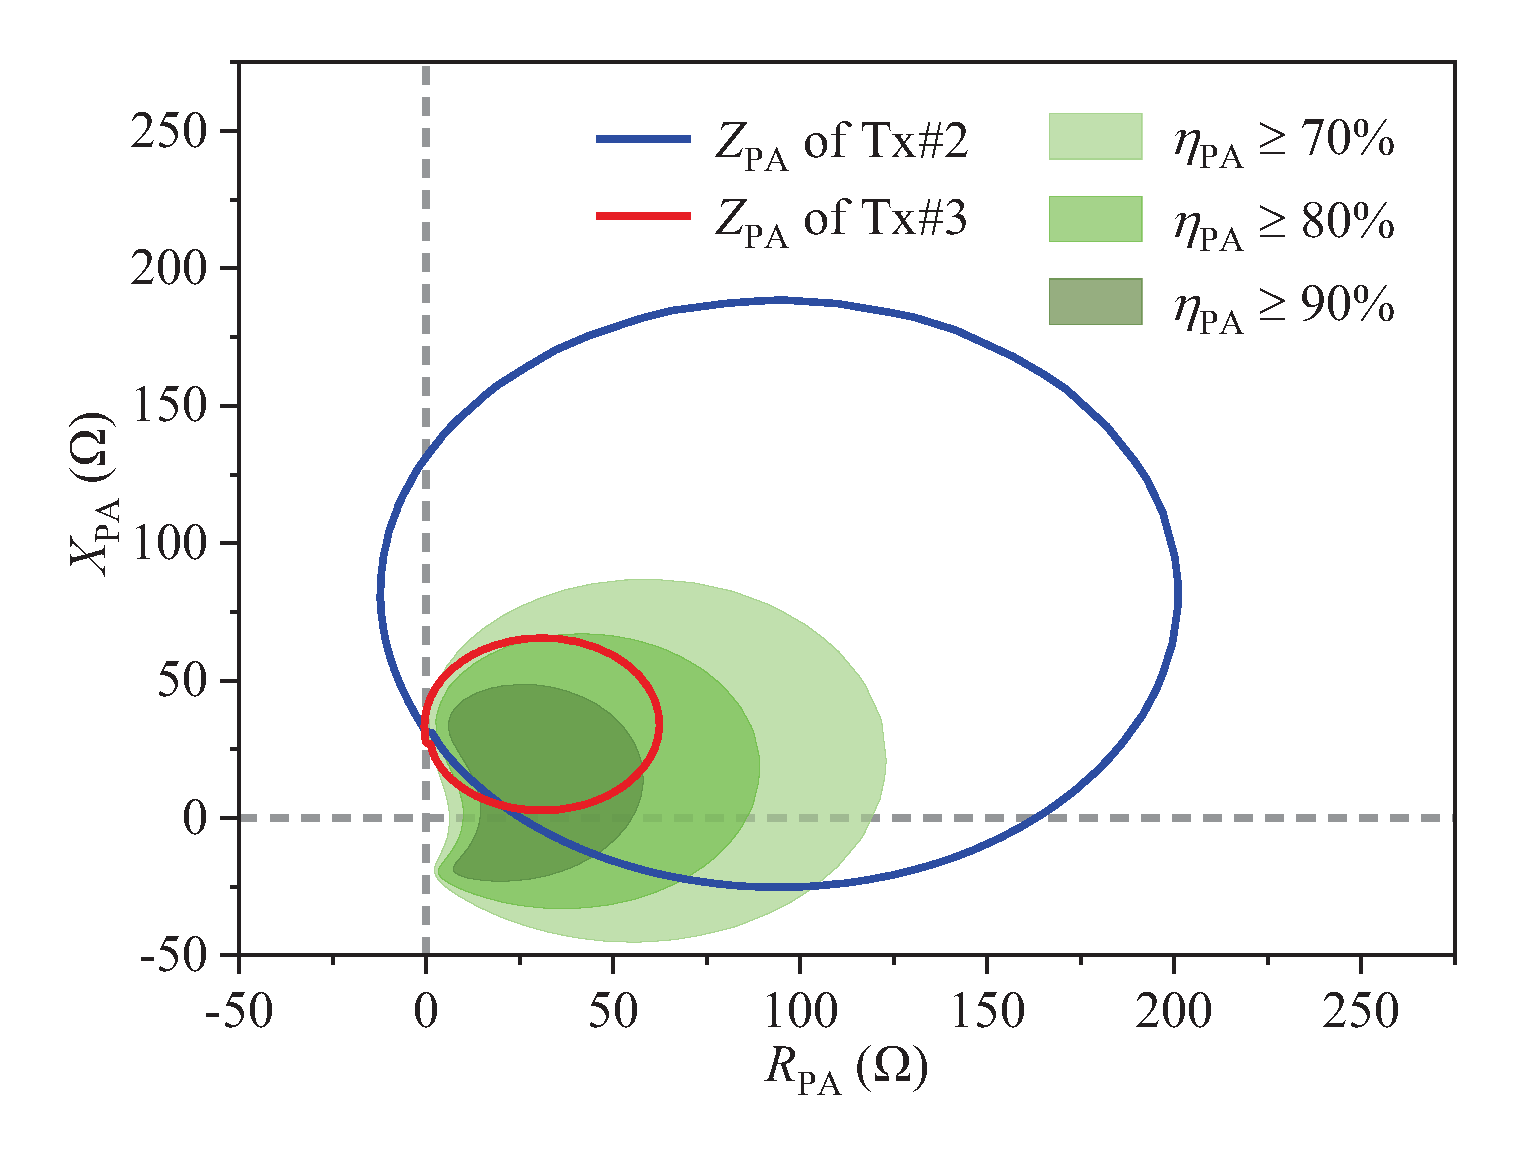
\includegraphics[width=8.0cm]{fig/fig13.eps}}
    \caption{Example PA load impedance trajectories ($\theta _{1}$=$\theta _{2}$=0, $\theta _{3}$ and $\theta _{4}$ are from 0 to 360 degrees).}
    \label{fig:impe}
\end{figure}

\subsection{Visualization of Magnetic Field Shaping}

To visualize the B-field strength distribution, an LED array with 25 receiving modules is built up. As shown in Fig.~\ref{systemled}, each receiving module is 2.5~cm$\times$2.5~cm, and the entire LED array is 20~cm$\times$20~cm. The supporting acrylic frame can fix the LED array in different positions and orientations through magnetic docking. Note that the lightness of the LEDs has a nonlinear relationship with the B-field strength.
\begin{figure}[ht!]
    \centering
    \centerline{\includegraphics[width=8.5cm]{fig/fig14.eps}}
    \caption{An LED array to visualize the magnetic field shaping.}
    \label{systemled}
\end{figure}

\begin{figure}[ht!]
    \centering
    \subfigure[]{
    \label{ex1}
    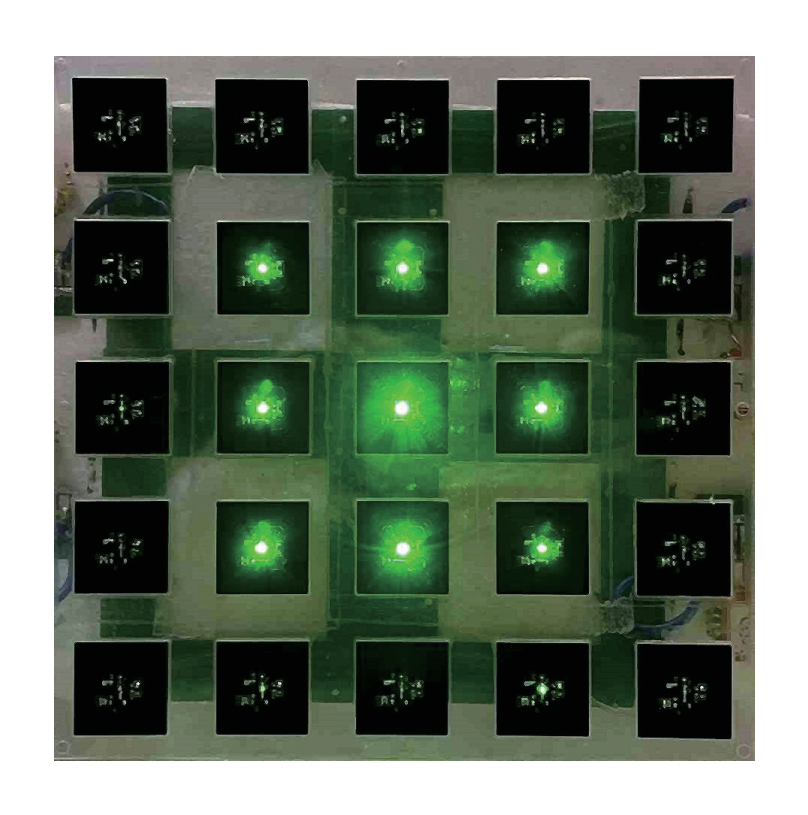
\includegraphics[height=3.3cm]{fig/fig15a.eps}}
    \hspace{0cm}
    \subfigure[]{
    \label{ex2}
    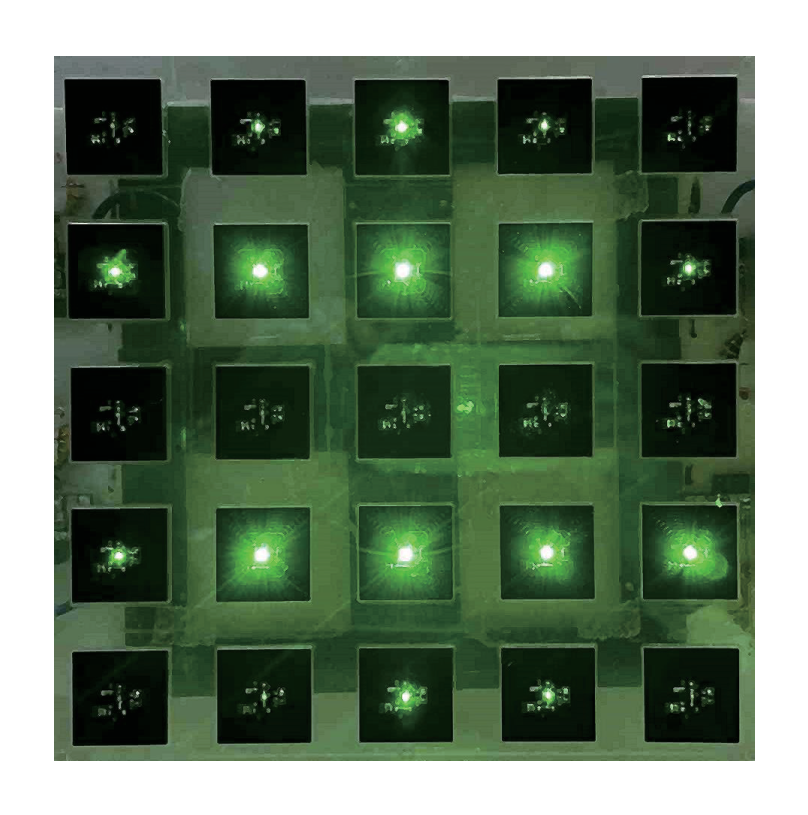
\includegraphics[height=3.3cm]{fig/fig15b.eps}}
    \subfigure[]{
    \label{eb1}
    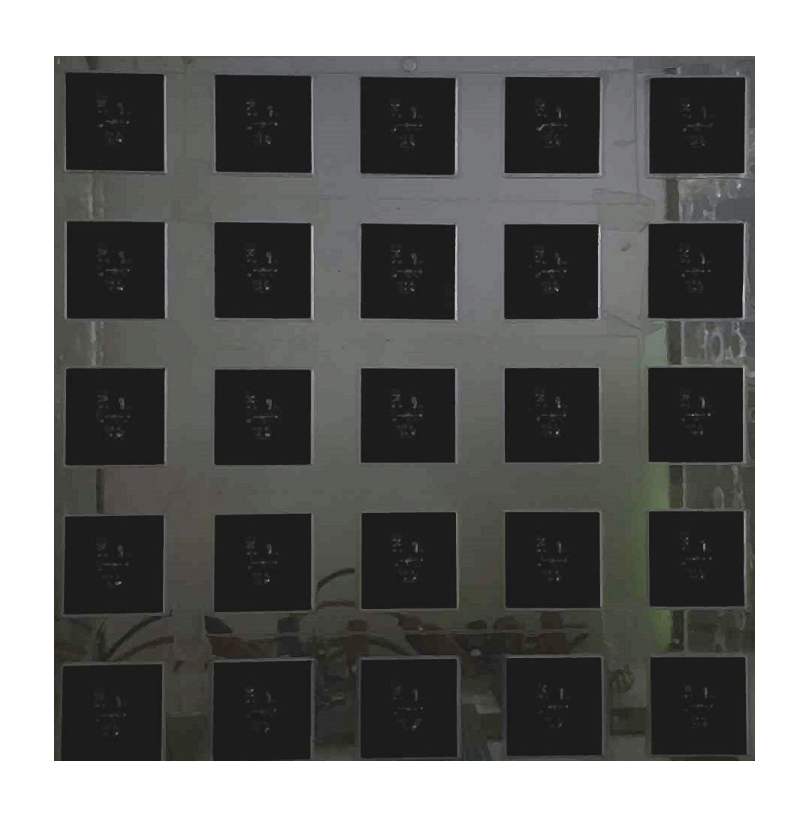
\includegraphics[height=3.3cm]{fig/fig15c.eps}}
    \hspace{0cm}
    \subfigure[]{
    \label{eb2}
    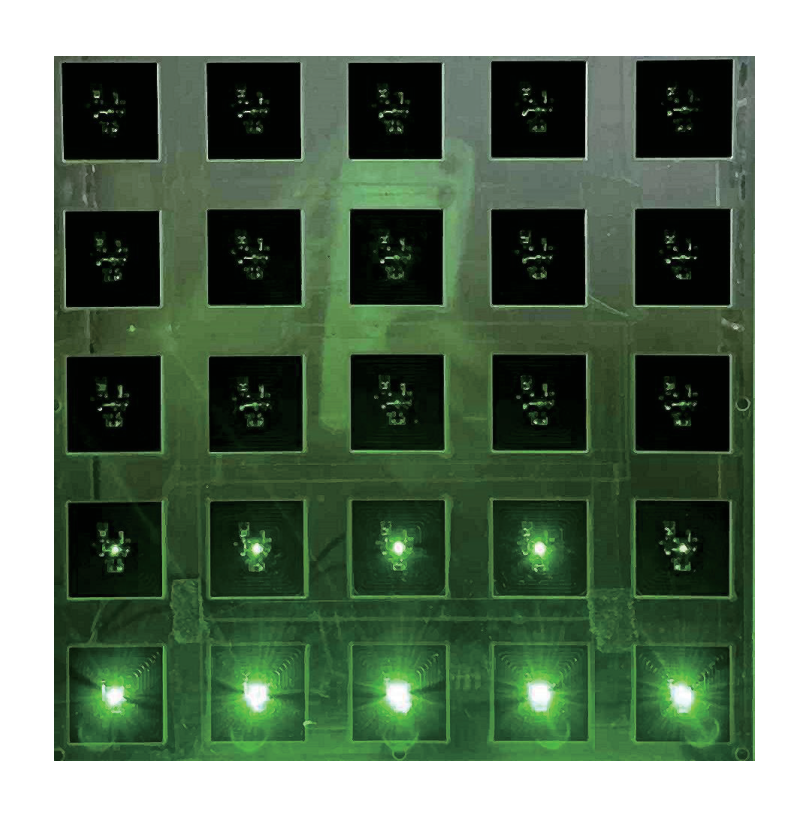
\includegraphics[height=3.3cm]{fig/fig15d.eps}}
    \caption{Illumination of the LED array in horizontal and perpendicular orientations.
    (a) Visualization corresponding to Fig.~\ref{x1} (horizontal). (b) Visualization corresponding to Fig.~\ref{x2} (horizontal). (c) Visualization corresponding to Fig.~\ref{b1} (perpendicular). (d) Visualization corresponding to Fig.~\ref{b2} (perpendicular).}
    \label{led}
\end{figure}
%\vspace{-5mm}

The four sub-figures in Fig.~\ref{led} correspondingly verify the calculation results in Fig.~\ref{x1}, Fig.~\ref{x2}, Fig.~\ref{b1}, and Fig.~\ref{b2}. The visualization results well match with their calculation results. Meanwhile, it is natural that there are minor differences, mostly due to the limited number of LED modules and nonlinearity between LED lightness and B-field strength. The above LED array is a convenient tool to directly visualize and confirm the actual magnetic field shaping effect.


\subsection{Rx Coil with Six Degrees of Freedom}

Fig.~\ref{6deg1} and Fig.~\ref{6deg2} show the measured output dc power and dc-dc efficiency using Tx\#1, Tx\#2 and Tx\#3. Note that Tx\#2 and Tx\#3 are the planar Tx-coil arrays without and with overlap, respectively. Experiments are conducted to investigate the performance when the Rx coil is in six-degrees-of-freedom positions and orientations~(i.e., $x$, $y$, $z$, $\alpha$, $\beta$ and $\gamma$). Due to the symmetry in ($x$, $y$) and ($\alpha$, $\beta$), their results are similar. To avoid redundancy, only the results for $x$, $z$, $\alpha$, and $\gamma$ cases are shown in the two figures. The input dc voltages of the three systems are all 20~V, and the driving signal phases of the four PAs ($\theta_1$--$\theta_4$) are accordingly modulated to investigate the magnetic field shaping effects. 

\begin{figure}[ht!]
    \centering
    %\vspace{-0.5cm}
    \subfigure[]{
    \label{xde}
    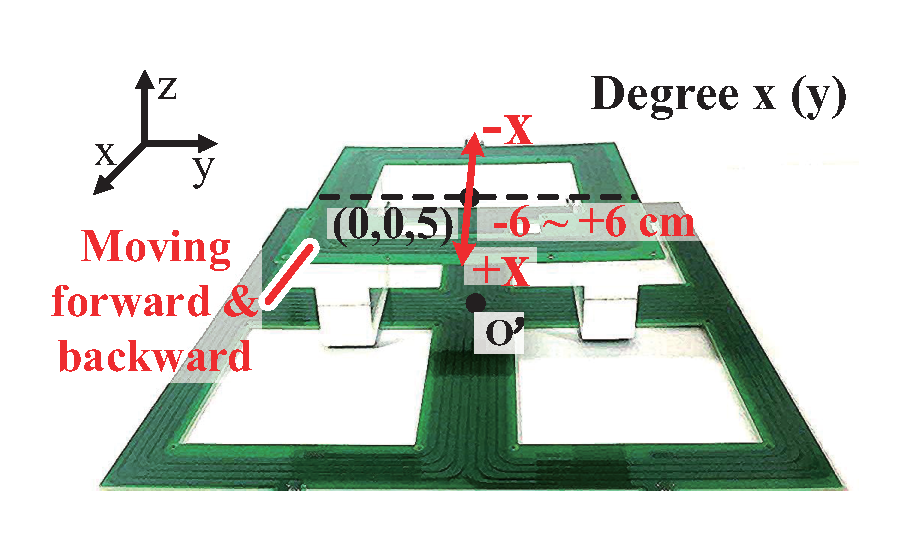
\includegraphics[height=2.5cm]{fig/fig16a.eps}}
    \subfigure[]{
    \label{zde}
    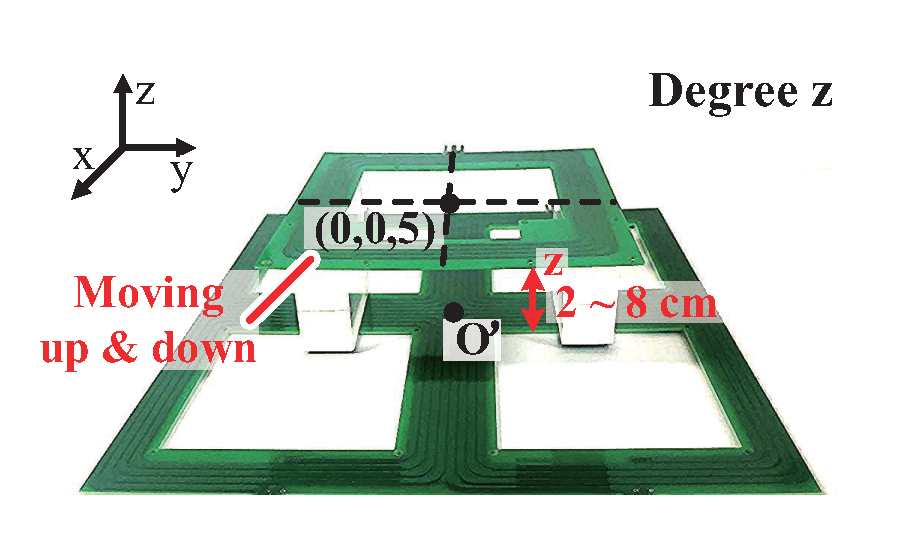
\includegraphics[height=2.5cm]{fig/fig16b.eps}}

    \subfigure[]{
    \label{xp}
    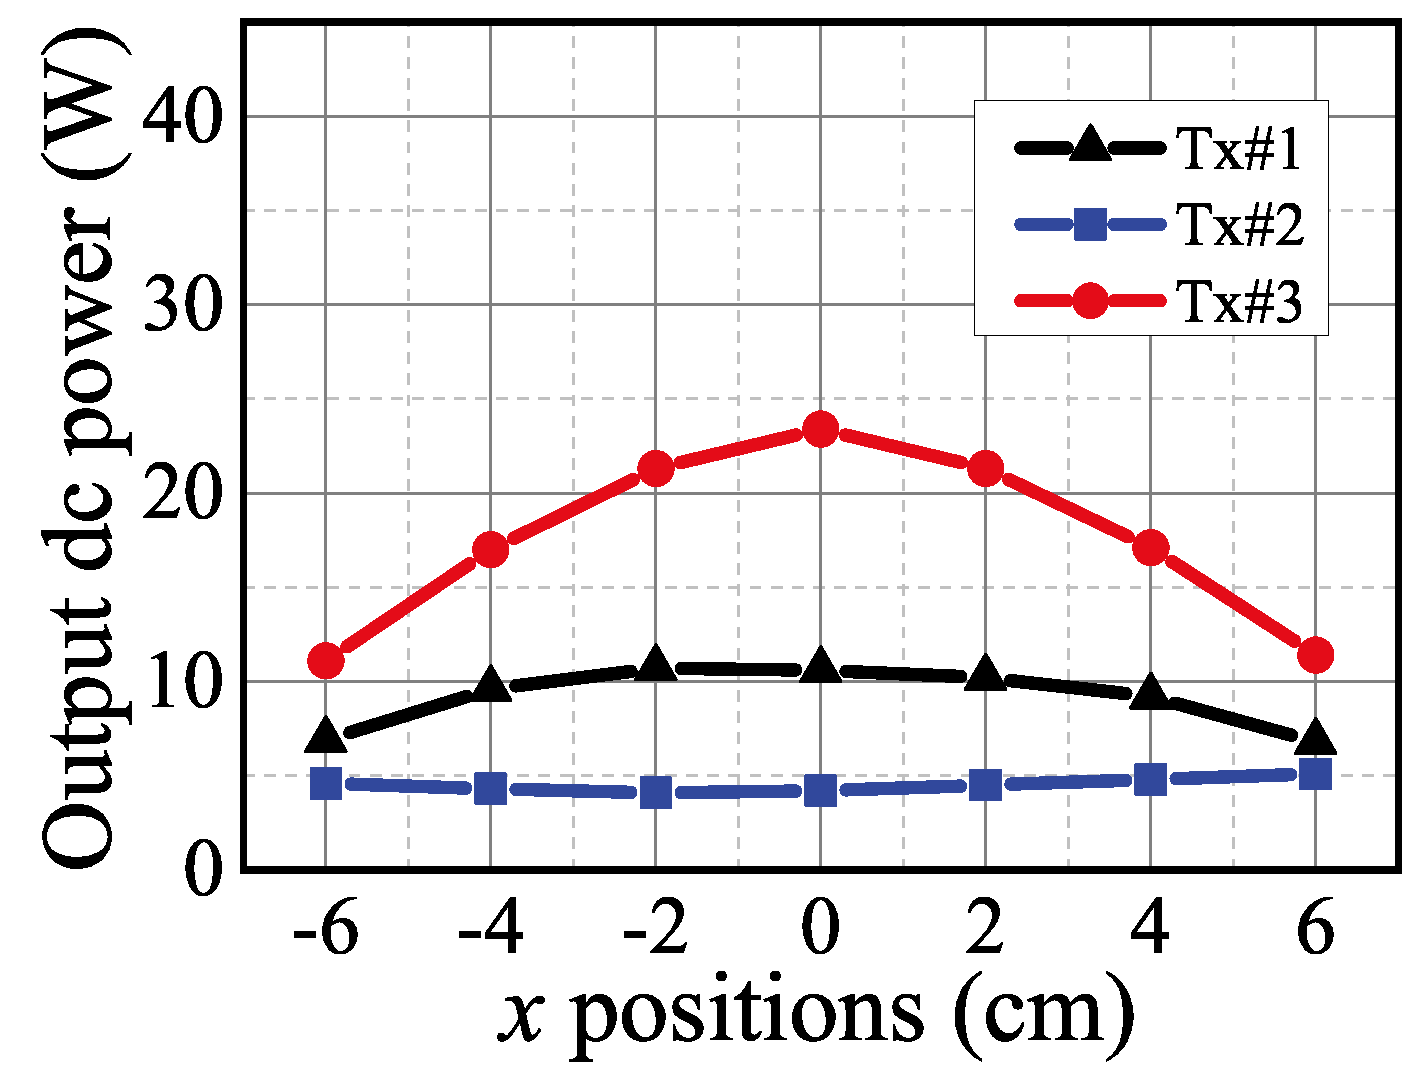
\includegraphics[height=2.8cm]{fig/fig16c.eps}}
    \hspace{2mm}
    \subfigure[]{
    \label{zp}
    \includegraphics[height=2.9cm]{fig/fig16d.eps}}

    \subfigure[]{
    \label{xe}
    \includegraphics[height=2.95cm]{fig/fig16e.eps}}
    \hspace{1mm}
    \subfigure[]{
    \label{ze}
    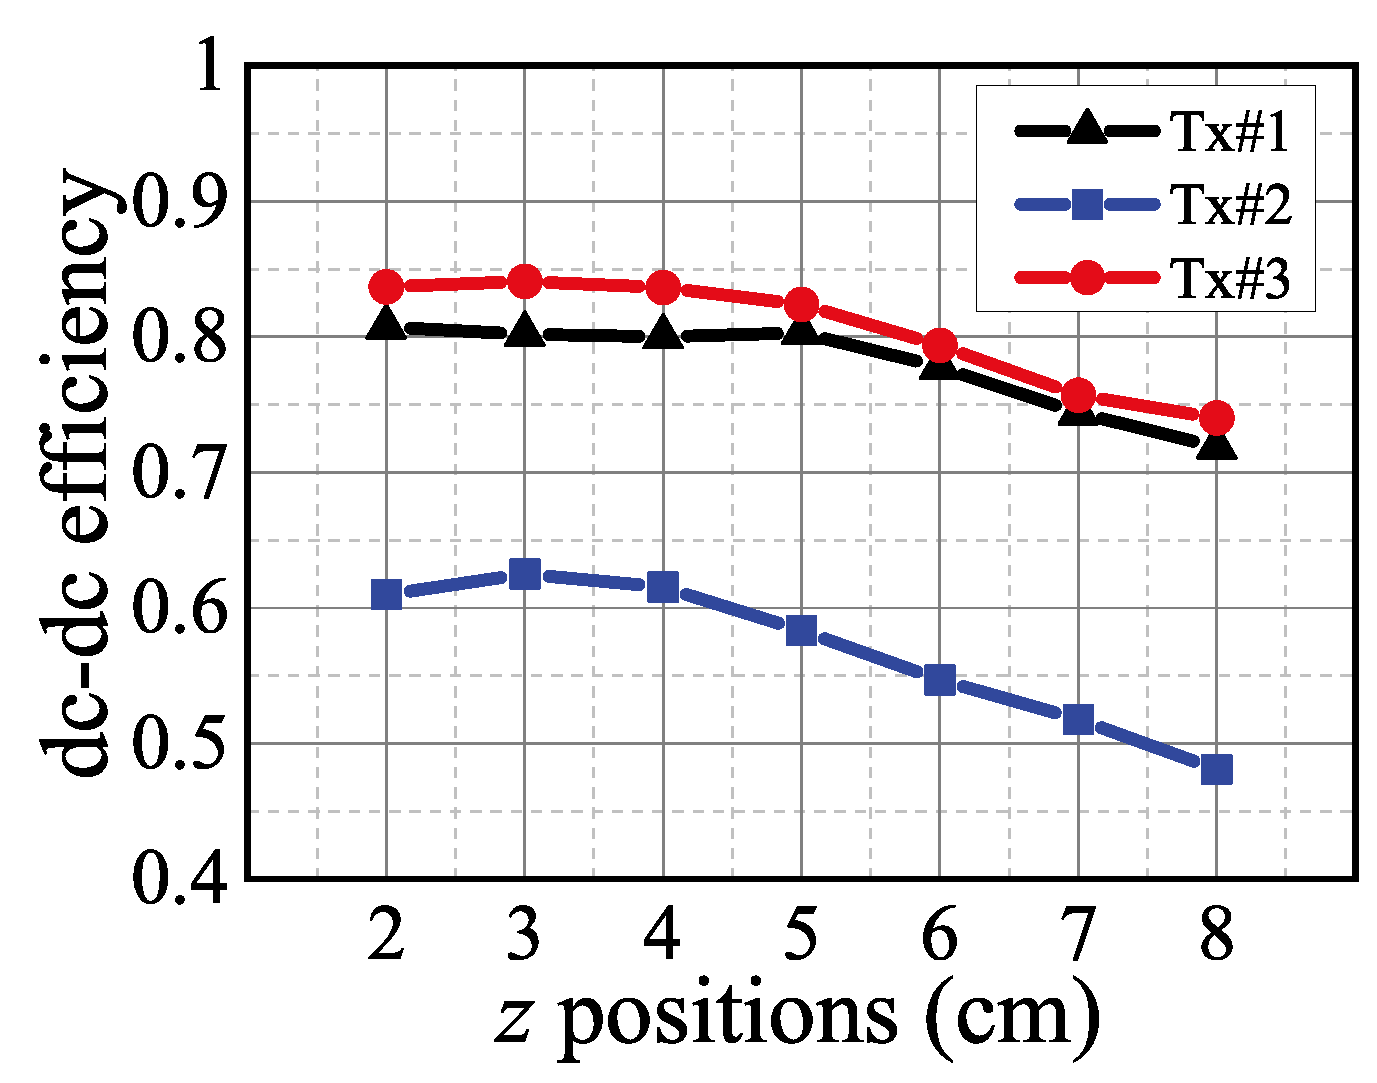
\includegraphics[height=2.95cm]{fig/fig16f.eps}}

    \caption{Experimental results in different $x$ and $z$ positions using Tx\#1, Tx\#2 and Tx\#3. (a) Setup~($x$ positions). (b) Setup~($z$ positions). (c) Output power~($x$ positions). (d) Output power~($z$ positions). (e) Dc-dc efficiency~($x$ positions). (f) Dc-dc efficiency~($z$ positions).}

    \label{6deg1}
\end{figure}
For the case of a moving Rx coil in $x$ direction ($\pm$6~cm), symmetrically placed Tx coils, (no.~1, no.~2) and (no.~3, no.~4), should have the same phase~[see Fig.~\ref{system}]. Therefore, here $\theta _{3}$ and $\theta _{4}$ are fixed to $0{}^{\circ}$, and $\theta_1$ and $\theta_2$ are tuned to change from $-180{}^{\circ}$ to $180{}^{\circ}$. For the movement of Rx in other directions, a similar principle is applied. Fig.~\ref{xp} shows that the output power using the Tx\#3 (i.e., the case with the overlap design) is obviously much higher than those using Tx\#1 and Tx\#2, while Tx\#1 (i.e., a single Tx coil) and Tx\#3 demonstrate the similar dc-dc efficiency. In Fig.~\ref{xe}, the efficiency in Tx\#3 case is extraordinary high when comparing with the Tx\#2 case (i.e., the case without coil overlap). The above results clearly show the importance of the overlap design for a high-performance MHz WPT system using the planar Tx-coil array. Otherwise, a large amount of power will be transferred among the Tx coils due to the cross coupling, which causes the lowest efficiency and output power in the Tx\#2 case. Similarly, the Tx\#3 coil array also demonstrated the best performance when the Rx coil moves along the $z$ axis~[see Fig.~\ref{zde}(d)(f)]. The Tx\#3 WPT system can achieve an 84\% dc-dc efficiency at 50~W. It can maintain the same output power 17.6~W as the maximum output power of the single Tx-coil WPT system (i.e., Tx\#1) but with a much longer transfer distance, about 6~cm versus 2~cm. Note that in the present scenario, the Rx coil moves vertically in the center. Thus phases $\theta_1$--$\theta_4$ are all zero~[see Fig.~\ref{z1}].

\begin{figure}[t!]
    \centering
    \subfigure[]{
    \label{ade}
    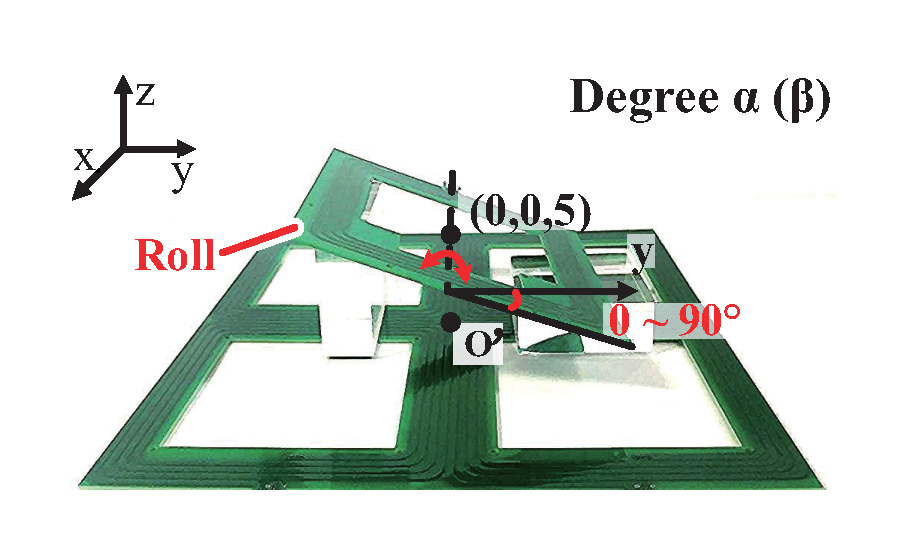
\includegraphics[height=2.45cm]{fig/fig17a.eps}}
    \subfigure[]{
    \label{rde}
    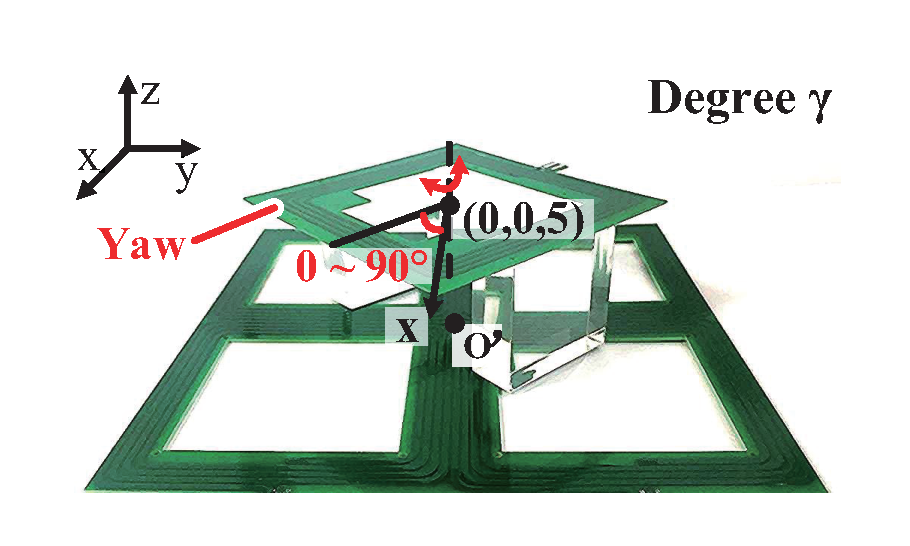
\includegraphics[height=2.45cm]{fig/fig17b.eps}}

    \subfigure[]{
    \label{ap}
    \includegraphics[height=2.9cm]{fig/fig17c.eps}}
    \hspace{2mm}
    \subfigure[]{
    \label{rp}
    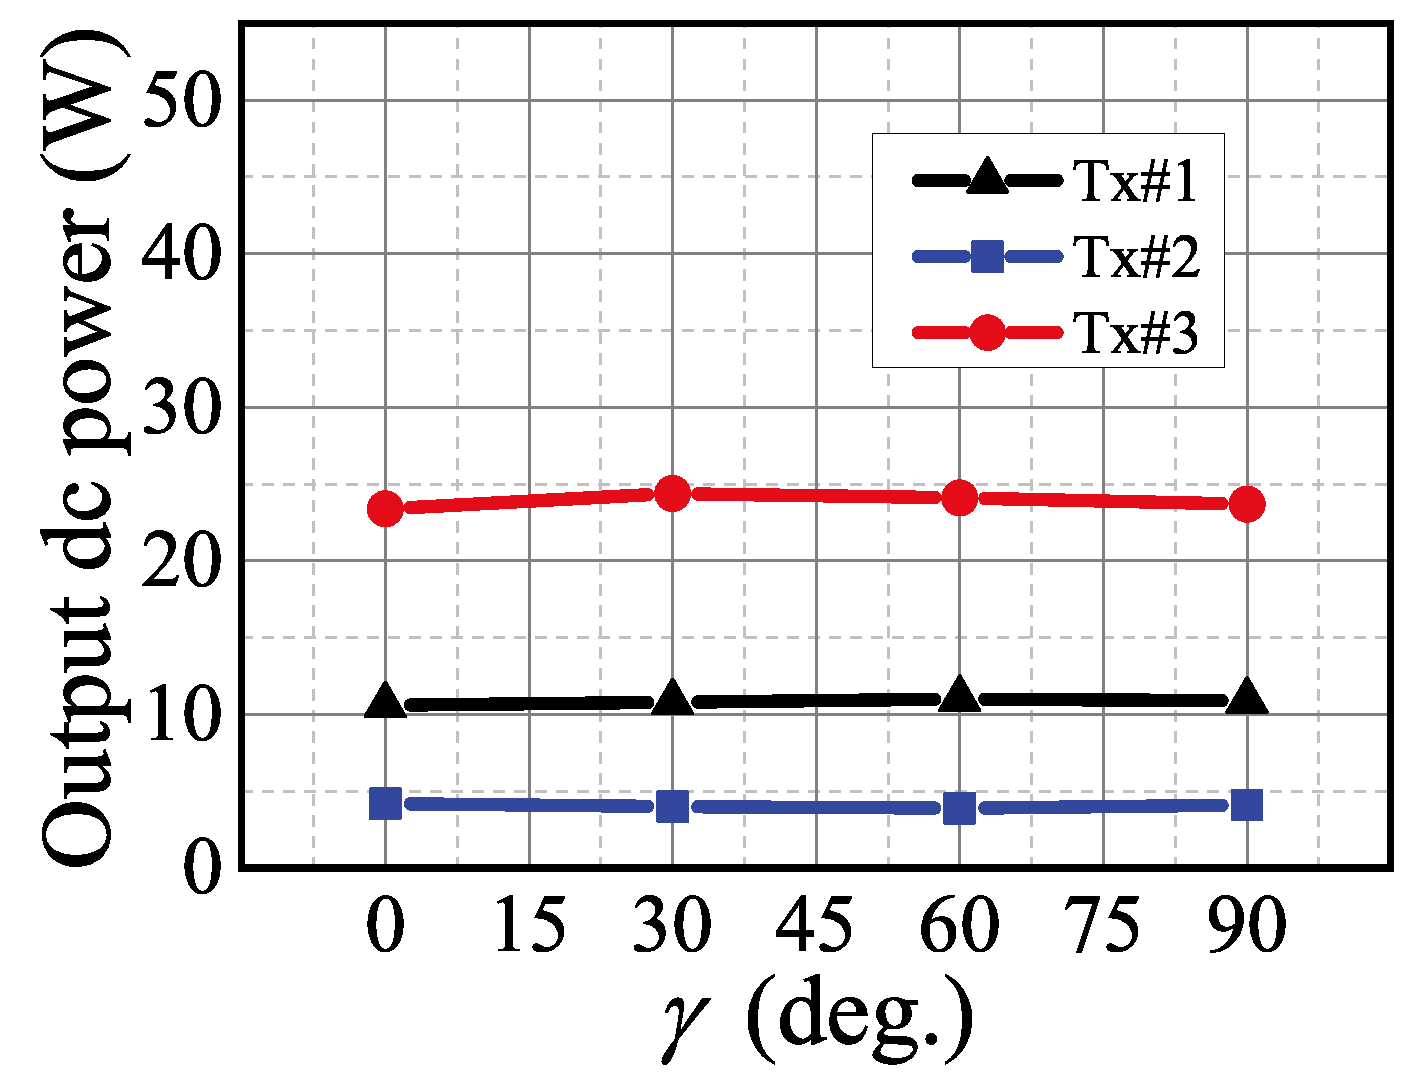
\includegraphics[height=2.8cm]{fig/fig17d.eps}}

    \subfigure[]{
    \label{ae}
    \includegraphics[height=2.95cm]{fig/fig17e.eps}}
    \hspace{1mm}
    \subfigure[]{
    \label{re}
    \includegraphics[height=2.95cm]{fig/fig17f.eps}}

    \caption{Experimental results in different $\alpha$ and $\gamma$ angles using Tx\#1, Tx\#2 and Tx\#3. (a) Setup~($\alpha$ angles). (b) Setup~($\gamma$ angles). (c) Output power~($\alpha$ angles). (d) Output power~($\gamma$ angles). (e) Dc-dc efficiency~($\alpha$ angles). (f) Dc-dc efficiency~($\gamma$ angles).}

    \label{6deg2}
\end{figure}
Fig.~\ref{6deg2} shows the results when the Rx coil rotates in $\alpha$ and $\gamma$ angles, i.e., with different orientations. Again, the results in $\beta$ angles are omitted due to their similarity with the results in $\alpha$ angles. For the case of $\alpha$ angles ($\alpha=0-90^{\circ}$), $\theta_2$ and $\theta_3$ are changed from $0^{\circ}$ to $-180^{\circ}$, while $\theta_1$ and $\theta_4$ are fixed to $0^{\circ}$. The results using the Tx\#3 coil array, namely Fig.~\ref{ap} and Fig.~\ref{ae}, demonstrate consistently the best performance, both in output power and efficiency. It is especially promising to notice that even when the Rx coil is perpendicular to the Tx coil array (i.e., $\alpha=90^{\circ}$), 45~W output power and 82\% dc-dc efficiency can still be achieved. Meanwhile, the conventional single Tx coil (i.e., Tx\#1) becomes completely unfunctional in such an extreme case because no magnetic flux will pass through the Rx coil. Note that the efficiency of the Tx\#2 case is also high when the Rx coil is perpendicular~[see Fig.~\mbox{\ref{ae}}]. This is mainly because that the PAs happenly see a suitable impedance reflected by other transmitters. The planar Tx-coil array, overlap design and phase shift modulation work together to provide new degrees of freedom in magnetic field shaping. The results using the Tx\#3 coil arrays in $\gamma$ angles are also superior in both output power and efficiency~[see Fig.~\ref{rp} and Fig.~\ref{re}].

\renewcommand\arraystretch{1.0}
\begin{table}[ht!]
\footnotesize
\caption{Additional Four Scenes (Tx\#3-Coil Array). }
\vspace{-6mm}
%\renewcommand{\arraystretch}{1}
\begin{center}
\resizebox{\columnwidth}{!}{
\begin{tabular}{c c l}
\toprule[1pt] \\[-1.8mm]
Scenes   & Rx Positions/Orientations  & Specs and Results    \\[0.8ex]
\midrule[0.5pt] %\\[-2mm]
\hspace{-4mm}
\begin{minipage}[b]{0.35\columnwidth}
		\centering
		\raisebox{-.5\height}{\includegraphics[width=1.0\linewidth]{fig/figTableIVa.eps}}
	\end{minipage}
& \makecell[c]{An eccentric\\perpendicular Rx}    & \makecell[l]{$\mathrm{\eta}_{\mathrm{dc}-\mathrm{dc}}=77.1\%$\\ $R_{\mathrm{L}}=10~\Omega$ \\ $P_{\mathrm{out}}=22.2~\mathrm{W}$}          \\
%\hline
\hspace{-4mm}
\begin{minipage}[b]{0.35\columnwidth}
		\centering
		\raisebox{-.5\height}{\includegraphics[width=1.0\linewidth]{fig/figTableIVb.eps}}
	\end{minipage}
& \makecell[c]{A randomly\\placed Rx}     & \makecell[l]{$\mathrm{\eta}_{\mathrm{dc}-\mathrm{dc}}=78.4\%$ \\ $R_{\mathrm{L}}=10~\Omega$ \\ $P_{\mathrm{out}}=16.3~\mathrm{W}$}             \\
\hspace{-4mm}
\begin{minipage}[b]{0.35\columnwidth}
		\centering
		\raisebox{-.5\height}{\includegraphics[width=1.0\linewidth]{fig/figTableIVc.eps}}
	\end{minipage}
& \makecell[c]{A perpendicular Rx\\and\\a horizontal Rx\\(Rx\#1: red, Rx\#2: yellow)}    & \makecell[l]{$\mathrm{\eta}_{\mathrm{dc}-\mathrm{dc}}=80.3\%$ \\ $R_{\mathrm{L},1}=10~\Omega$ \\ $P_{\mathrm{out},1}=20.4~\mathrm{W}$ \\ $R_{\mathrm{L},2}=5~\Omega$ \\ $P_{\mathrm{out},2}=14.7~\mathrm{W}$}              \\
\hspace{-4mm}
\begin{minipage}[b]{0.35\columnwidth}
		\centering
		\raisebox{-.5\height}{\includegraphics[width=1.0\linewidth]{fig/figTableIVd.eps}}
	\end{minipage}
& \makecell[c]{Two horizontal Rxs\\(Rx\#1: red, Rx\#2: yellow)}     & \makecell[l]{$\mathrm{\eta}_{\mathrm{dc}-\mathrm{dc}}=81.4\%$ \\ $R_{\mathrm{L},1}=10~\Omega$ \\ $P_{\mathrm{out},1}=18.0~\mathrm{W}$ \\ $R_{\mathrm{L},2}=5~\Omega$ \\ $P_{\mathrm{out},2}=12.6~\mathrm{W}$}   \\
[0.3ex]
\bottomrule[1pt]
\end{tabular}
}
\label{new4}
\end{center}
%\vspace{-4mm}
\end{table}

\subsection{Further discussions}

The results of additional four scenes are summarized in Table~\ref{new4}, using the optimally designed Tx\#3-coil array to reduce the cross coupling between the Tx coils. Note that for clarity, the circuits (PAs, rectifiers, etc.) are not shown in the figures. Again, the results are promising in terms of efficiency and output power. Especially, in the third scene, the perpendicular Rx\#1 and horizontal Rx\#2 provide output powers of 20.4~W and 14.7~W, respectively. The overall dc-dc efficiency is as high as 80.3\%. In actual scenarios, a perpendicular Rx can be convenient for the wireless charging of smart watches, headsets, hand-held cellphones, etc. In such applications, the charging surface of the mobile devices may be placed upright. All the above results indicate that in a wide range of new applications, a well-designed and controlled planar Tx-coil array could further improve the spatial freedom of today's WPT. 

\begin{figure}[ht!]
    \centering
    \centerline{\includegraphics[width=8.5cm]{fig/fig18.eps}}
    \caption{Experimental current waveforms of the four Tx coils (0.7~A/div, 150~ns/div).}
    \label{Iorigin}
\end{figure}
Fig.~\ref{Iorigin} shows the experimental current waveforms of the four Tx coils in Fig.~\ref{system}, i.e., with a perpendicular Rx coil in the center. The phases of the driving signals are $0{}^{\circ}$, $0{}^{\circ}$, $-180{}^{\circ}$, and $-180{}^{\circ}$. Offsets are observed in the actual Tx current phases, as shown in Fig.~\ref{Iorigin}. This is mainly because that the cross coupling is largely reduced, but is not completely eliminated. Meanwhile, the final MHz WPT system still performs well, as mentioned above. Further reduction of the cross coupling should be investigated in the future, and it is also possible to develop a feedback-based compensation scheme of the driving signals to eventually achieve accurate phase shift modulation of final Tx currents.

\begin{table*}[htbp]%\small
  \renewcommand\arraystretch{1.3}
  \centering
  \caption{Comparison of WPT systems with Magnetic Field Shaping.}
  \begin{threeparttable}
    \begin{tabular}{c|ccccc|c}
    \toprule[1pt]
    Reference & 2014~\cite{ng2014two} & 2016~\cite{zhang2015basic} & 2018~\cite{zhu2017field} & 2020~\cite{zhang2019angular} & 2021~\cite{feng2021load} & This Work \\
    \cmidrule[0.4pt](lr){1-1} \cmidrule[0.4pt](lr){2-6} \cmidrule[0.4pt](lr){7-7}
    Output Power & 3~W    & 1.07~W & 13.7~W & 8 - 18~W & 3 - 15~W & 9 - 50~W \\
    Efficiency & 50\% - 60\% & 69.5\% & 28.2\% & 60\% - 65\% & 60\% - 70\%\tnote{*} & 74\% - 84\%\tnote{*} \\
    Operating Frequency & 530 kHz & 550 kHz & 20 kHz & 100 kHz & 6.78 MHz & 6.78 MHz \\
    Spatial DoF of Rx & 3     & 3     & 3     & 3     & 6     & 6 \\
    Tx-coil Structure & Spherical Shape & Spherical Shape & Cubic Shape & Spherical Shape & Bowl Shape & \makecell[c]{Extendable 2D \\ Coil Array} \\
    \makecell[c]{Cross Coupling \\ Minimization} & \makecell[c]{Orthogonal \\ Coils} & \makecell[c]{Orthogonal \\ Coils} & \makecell[c]{Orthogonal \\ Coils} & \makecell[c]{Orthogonal \\ Coils} & \makecell[c]{--} & Overlap Design \\
    \bottomrule[1pt]
    \end{tabular}%
 		\begin{tablenotes}
        	\footnotesize
        	\item[*]: dc-dc efficiency.
      	\end{tablenotes}
  \end{threeparttable}
  \label{tab:vs}%
\end{table*}%
Finally, Table~\ref{tab:vs} summarizes the specifications and performance of state-of-the-art WPT systems with magnetic field shaping. As shown by the comparison, the developed system in this paper demonstrated improved power transfer capability and dc-dc efficiency at 6.78~MHz. Thanks to the proposed overlap design to minimize the cross coupling between the Tx coils, it becomes possible to realize effective 3D magnetic field shaping using an extendable 2D planar Tx-coil array.


\section{Conclusion}
\label{sec:conclusion}

This paper studies the planar Tx-coil array architecture and current phase shift modulation technique to realize the magnetic field shaping in 3D space. The B-field amplitude distribution is analytically derived based on the Biot-Savart law and phasor representation. In order to reduce the interference to the PA operation, the influence of the cross coupling between the Tx coils is especially analyzed and minimized. Both the calculation and experimental results have well verified the effect of the magnetic field shaping under different current phases of individual Tx coils, and demonstrated significantly improved spatial freedom of power transfer to receivers in different 3D positions and orientations. 

Based on the above promising results, main future works may include 1) 3D position and orientation detection of Rx coils; 2) real-time phase shift modulation for power transfer to a moving receiver; 3) scheme and analysis of multiple-receiver power transfer in 3D space, etc. Especially, a ``scan" mechanism can be developed to drive the Tx coils sequentially in a certain pattern. The different reflected impedances seen by the individual Tx coils could be utilized to reconstruct the 3D location and orientation of an Rx coil. The optimal phase shift in each Tx coil can then be calculated based on the derived B-field amplitude distribution functions (ADFs), following specific design targets such as maximizing power transfer efficiency and capability.

\appendix
	The $x$-direction, $y$-direction and $z$-direction components of the B-field induced by Tx$_{i,j}$ at P$\left(x,y,z\right)$ are derived and listed in Table~\ref{Bcomponents}. Here $B_{\left\{ \bullet \right\}}|_{i,j}$ represents $B_x|_{i,j}$, $B_y|_{i,j}$ or $B_z|_{i,j}$. %\\
	
\begin{table*}[ht]
	\renewcommand{\arraystretch}{1.2}
	%\renewcommand{\multirowsetup}{\centering}
	\caption{x-, y-, and z-direction Components of B-field Induced by Tx$_{i,j}$ Coil at P$\left(x,y,z\right)$.}
	%\centering
	\vspace{-1mm}
	\label{Bcomponents}
	%\centering
	%\resizebox{\columnwidth}{!}{
		\begin{tabular}{c c c}
			\toprule[1pt] \\[-3mm]
			\multicolumn{1}{c}{$\overline{B}$} & \multicolumn{1}{c}{$B_{\left\{ \bullet \right\}}|_{i,j}$} & \multicolumn{1}{c}{{Derivation}}  \\[1.1ex]
			\midrule[0.5pt] \\[-2mm]

			\multirow{2}{*}[-10pt]{ $ \overline{B_{{i,j}}} $}&\multirow{2}{*}[-10pt]{$B_x|_{i,j}$}&
            $\frac{\mu _0 N_{tx} I_{i,j}^m \cos \left(\omega t + \theta_{i,j} \right)}{4 \pi } \left\{\frac{z}{[j (d+l)-x]^2+z^2}\left\{\frac{y-i (d+l)}{\left\{[j (d+l)-x]^2+[i (d+l)-y]^2+z^2\right\}^{\frac{1}{2}}}+\frac{i (d+l)-l-y}{\left\{[j (d+l)-x]^2+[i (d+l)-l-y]^2+z^2\right\}^{\frac{1}{2}}}\right\}+\right.$\\
            & & $\left.\frac{z}{[j (d+l)-l-x]^2+z^2}\left\{\frac{i (d+l)-y}{\left\{[j (d+l)-l-x]^2+[i (d+l)-y]^2+z^2\right\}^{\frac{1}{2}}}+\frac{-i (d+l)+l+y}{\left\{[j (d+l)-l-x]^2+[i (d+l)-l-y]^2+z^2\right\}^{\frac{1}{2}}}\right\}\right\}$  \\[2.0ex]
            \\[-2mm]

			\multirow{2}{*}{}&\multirow{2}{*}[-10pt]{$B_y|_{i,j}$}&
            $\frac{\mu _0 N_{tx} I_{i,j}^m \cos \left(\omega t + \theta_{i,j} \right)}{4 \pi } \left\{\frac{-z}{[i (d+l)-y]^2+z^2}\left\{\frac{j (d+l)-x}{\left\{[j (d+l)-x]^2+[i (d+l)-y]^2+z^2\right\}^{\frac{1}{2}}}+\frac{-j (d+l)+l+x}{\left\{[j (d+l)-l-x]^2+[i (d+l)-y]^2+z^2\right\}^{\frac{1}{2}}}\right\}+\right.$\\
            &&$\left.\frac{z}{[i (d+l)-l-y]^2+z^2}\left\{\frac{j (d+l)-x}{\left\{[j (d+l)-x]^2+[i (d+l)-l-y]^2+z^2\right\}^{\frac{1}{2}}}+\frac{-j (d+l)+l+x}{\left\{[j (d+l)-l-x]^2+[i (d+l)-l-y]^2+z^2\right\}^{\frac{1}{2}}}\right\}\right\}$  \\[2.0ex]
            \\[-2mm]

			\multirow{4}{*}{}&\multirow{4}{*}[-20pt]{$B_z|_{i,j}$}&
            $\frac{\mu _0 N_{tx} I_{i,j}^m \cos \left(\omega t + \theta_{i,j} \right)}{4 \pi } \left\{\frac{y-i (d+l)}{[i (d+l)-y]^2+z^2}\left\{\frac{j (d+l)-x}{\left\{[i (d+l)-y]^2+[j (d+l)-x]^2+z^2\right\}^{\frac{1}{2}}}+\frac{-j (d+l)+l+x}{\left\{[i (d+l)-y]^2+[j (d+l)-l-x]^2+z^2\right\}^{\frac{1}{2}}}\right\}+\right.$\\
            &&$\frac{j (d+l)-l-x}{[j (d+l)-l-x]^2+z^2}\left\{\frac{i (d+l)-y}{\left\{[i (d+l)-y]^2+[j (d+l)-l-x]^2+z^2\right\}^{\frac{1}{2}}}+\frac{-i (d+l)+l+y}{\left\{[i (d+l)-l-y]^2+[j (d+l)-l-x]^2+z^2\right\}^{\frac{1}{2}}}\right\}- $ \\
            && $\frac{j (d+l)-x}{[j (d+l)-x]^2+z^2}\left\{\frac{i (d+l)-y}{\left\{[i (d+l)-y]^2+[j (d+l)-x]^2+z^2\right\}^{\frac{1}{2}}}+\frac{-i (d+l)+l+y}{\left\{[i (d+l)-l-y]^2+[j (d+l)-x]^2+z^2\right\}^{\frac{1}{2}}}\right\}- $ \\
            && $\left.\frac{-i (d+l)+l+y}{[i (d+l)-l-y]^2+z^2}\left\{\frac{j (d+l)-x}{\left\{[i (d+l)-l-y]^2+[j (d+l)-x]^2+z^2\right\}^{\frac{1}{2}}}+\frac{-j (d+l)+l+x}{\left\{[i (d+l)-l-y]^2+[j (d+l)-l-x]^2+z^2\right\}^{\frac{1}{2}}}\right\}\right\}$ \\[1.4ex]
            \\[-2mm]
			\bottomrule[1pt]
		\end{tabular}
	%}
	%\vspace{3mm}
\end{table*}

%\newpage
%\balance
\bibliographystyle{Bibliography/IEEEtranTIE}
\bibliography{Bibliography/IEEEabrv,Bibliography/myRef}
%\bibliographystyle{IEEEtran}
%\bibliography{Bibliography/myRef}\ %IEEEabrv instead of IEEEfull

\begin{IEEEbiography}[{\includegraphics[width=1in,height=1.25in,clip,keepaspectratio]{NingKang.eps}}]{Ning Kang}(S'18) received the B.S. degree in information engineering with National Scholarship Honors from Nanjing University of Aeronautics and Astronautics, Nanjing, China, in 2017. He is currently working toward the Ph.D. degree in electrical and computer engineering with the University of Michigan-Shanghai Jiao Tong University Joint Institute, Shanghai Jiao Tong University, Shanghai, China.

His research interests include design and control strategies of megahertz wireless power transfer systems, such as multiple-transmitter systems under FPGA high-speed control.

\end{IEEEbiography}

\begin{IEEEbiography}[{\includegraphics[width=1in,height=1.25in,clip,keepaspectratio]{YaoxiaShao.eps}}]{Yaoxia Shao}(S'19) received the B.S. degree in mechanical design, manufacturing and automation from Tongji University, Shanghai, China, in 2018. He is currently working toward the Ph.D. degree in electrical and computer engineering at the University of Michigan-Shanghai Jiao Tong University Joint Institute, Shanghai Jiao Tong University, China.
	
His research interests include high-frequency power conversion circuits and applications in both inductive power transfer and microwave power transfer.
\end{IEEEbiography}

\begin{IEEEbiography}[{\includegraphics[width=1in,height=1.25in,clip,keepaspectratio]{MingLiu.eps}}]{Ming Liu}(S'15-M'17-SM'21) received the B.S. degree in mechatronic engineering from Sichuan University, Sichuan, China, in 2007, and the Ph.D. degree in electrical and computer engineering from the University of Michigan-Shanghai Jiao Tong University Joint Institute, Shanghai Jiao Tong University, Shanghai, China, in 2017.

From 2017 to 2020, he was a Postdoctoral Research Fellow with the Department of Electrical Engineering, Princeton University, USA. He joined the School of Electronic Information and Electrical Engineering, Shanghai Jiao Tong University, Shanghai, China, in 2020, where he is currently an Associate Professor of Electrical Engineering. His research interests include megahertz wireless power transfer, battery management systems, high frequency high performance power electronics for emerging applications.

Dr. Liu was the recipient of Top Ten Academic Star Award and Excellent PhD Thesis Award Nomination from Shanghai Jiao Tong University in 2016 and 2018, Research Excellence Award from AirFuel Alliance, USA, in 2019,
Best Paper Award of IEEE ECCE-Asia in 2020, and Best Student Paper Prize of IEEE WoW in 2021 with his student. He serves as the Chair of the Wireless Power Transfer for Energy Storage Charging Subcommittee of Energy Storage Technical Committee, IEEE Industrial Electronics Society.
\end{IEEEbiography}

\begin{IEEEbiography}[{\includegraphics[width=1in,height=1.25in,clip,keepaspectratio]{ChengbinMa.eps}}]{Chengbin Ma}(M'05-SM'18) received the B.S. degree in industrial automation from East China University of Science and Technology, Shanghai, China, in 1997, and the M.S. and Ph.D. degrees in electrical engineering from the University of Tokyo, Tokyo, Japan, in 2001 and 2004, respectively.

From 2004 to 2006, he was an R\&D Researcher with the Servo Motor Laboratory, FANUC Limited, Japan. Between 2006 and 2008, he was a Postdoctoral Researcher with the Department of Mechanical and Aeronautical Engineering, University of California, Davis, USA. In 2008, he joined the University of Michigan-Shanghai Jiao Tong University Joint Institute, Shanghai Jiao Tong University, Shanghai, China, where he is currently an Associate Professor of Electrical and Computer Engineering. His research interests include battery and energy management, wireless power transfer, dynamics and motion control, and wide applications in electronic devices, electric vehicles, microgrids, smart grids, etc.

Dr. Ma was the recipient of many teaching and research awards at Shanghai Jiao Tong University, such as Teaching and Education Award in 2020 and Koguan Top Ten Best Teacher Award in 2017. He also received Research Excellence Award from AirFuel Alliance, USA, in 2019. He is an Associated Editor for the IEEE Transactions on Industrial Informatics and IEEE Journal of Emerging and Selected Topics in Industrial Electronics. He served as Delegate of Energy Cluster (2019-20), and is now Chair of Shanghai Chapter, IEEE Industrial Electronics Society.
\end{IEEEbiography}

\end{document}
